%\documentclass[handout]{beamer}
\documentclass[lecture]{beamer}

%\usepackage[latin1]{inputenc}
\usepackage{pifont,amsmath,amssymb,amsfonts,euscript,mathrsfs,wasysym,textcomp}
\usepackage{psfrag}
\usepackage{multimedia}
\usepackage{fancybox}
\usepackage{soul}
\usetheme{Boadilla}
\usepackage{xcolor}

\usepackage{array}
\usepackage{calc}

\usepackage{pgf}
\usepackage{tikz}
\usepackage[utf8]{inputenc}
\usetikzlibrary{arrows,automata}
\usetikzlibrary{positioning}
\usetikzlibrary{calc}
\usepackage{amsmath}

\newcommand {\cmatr}[2]{\left\{\begin{array}{#1}#2\end{array}\right.}

\makeatletter
\newcommand{\pushright}[1]{\ifmeasuring@#1\else\omit\hfill$\displaystyle#1$\fi\ignorespaces}
\newcommand{\pushleft}[1]{\ifmeasuring@#1\else\omit$\displaystyle#1$\hfill\fi\ignorespaces}
\makeatother

\DeclareMathOperator*{\argmax}{arg\,max}
\DeclareMathOperator*{\argmin}{arg\,min}



\newcommand{\highlightred}[1]{%
  \colorbox{red!50}{$\displaystyle#1$}}
  \newcommand{\highlightgreen}[1]{%
  \colorbox{green!50}{$\displaystyle#1$}}
\usepackage{pgfpages}
%\pgfpagesuselayout{4 on 1}[a4paper,landscape,border shrink=5mm]
%\pgfpagesuselayout{2 on 1}[letterpaper,border shrink=5mm]
\usepackage{mathtools}

\setbeamertemplate{blocks}[rounded][shadow=false]

\newtheorem{Proposition}{Proposition}

\usepackage{tikz}
\usetikzlibrary{arrows,shapes}
\tikzstyle{na} = [baseline=-.5ex]
\tikzstyle{every picture}+=[remember picture]
\usetikzlibrary{positioning,intersections}

\makeatletter
\def\hlinewd#1{%
\noalign{\ifnum0=`}\fi\hrule \@height #1 %
\futurelet\reserved@a\@xhline}
\makeatother



\newsavebox{\fmbox}
\newenvironment{fmpage}[1]
  {\begin{lrbox}{\fmbox}\begin{minipage}{#1}}
  {\end{minipage}\end{lrbox}\fbox{\usebox{\fmbox}}}

\newcommand\BackgroundPicture[1]{%
   \setbeamertemplate{background}{%
   \parbox[c][\paperheight]{\paperwidth}{%
       \vfill \hfill
        \includegraphics[width=1\paperwidth,height=1\paperheight]{#1}
        \hfill \vfill
}}}

\definecolor{myGreen}{rgb}{0.,0.4,0.}
\definecolor{myGreen2}{rgb}{0.,0.8,0.}
\definecolor{myGreen3}{rgb}{0.,0.6,0.}
\definecolor{myLightGreen}{rgb}{0.9,1,0.9}
\definecolor{myBlue}{rgb}{0.,0.,0.4}
\definecolor{myBlue2}{rgb}{0,0.1,0.6}
\definecolor{myOrange}{rgb}{1.,0.5,0.}
\definecolor{myBrown}{rgb}{.65,.16,.15}
\definecolor{myCyan}{rgb}{.65,.16,.15}
\definecolor{myPurple}{rgb}{1,0,1}
\definecolor{myRed}{rgb}{0.8,0,0}
\definecolor{myRed2}{rgb}{0.65,0,0}
\definecolor{deepBlue}{rgb}{0.0,0,1}

\definecolor{myLightBlue}{rgb}{0.9,0.9,1}
\definecolor{myLightRed}{rgb}{1,0.9,0.9}


\newcommand{\FSII}{1}
\newcommand{\FSIII}{0.8}




\newcommand {\condmatr}[2]{\left\{\begin{array}{#1}#2\end{array}\right.}
\newcommand{\defi}{\stackrel{\footnotesize\Delta}{=}}
\newcommand{\expon}[1]{\ensuremath{\textnormal{e}^{#1}}}
\newcommand{\RR}{\textnormal{\textsf{I}\!\textsf{R}}}
\newcommand{\ini}[1]{\ensuremath{#1_{k}}}
\newcommand{\fin}[1]{\ensuremath{#1_\textnormal{f}}}
\newcommand{\der}[1]{\textnormal{d}{#1}}
\newcommand{\derk}[2]{\textnormal{d}^{#1}#2}
\newcommand{\ddt}[1]{\frac{\der{#1}}{\der{t}}} 
\newcommand{\dkdtk}[2]{\frac{\derk{#1}{#2}}{\der{t}^{#1}}} 
\newcommand{\dd}[2]{\frac{\der{#1}}{\der{#2}}} 
\newcommand{\NN}{\ensuremath{\textnormal{\textsf{I}\!\textsf{N}}}}
\newcommand {\matr}[2]{\left[\begin{array}{#1}#2\end{array}\right]}
\newcommand {\omatr}[2]{\begin{array}{#1}#2\end{array}}
%\newcommand{\Rn}[1]{\ensuremath{\RR^{#1}}}
%\newcommand{\En}[1]{\ensuremath{E_{#1}}}
\newcommand{\En}[1]{\ensuremath{\RR^{#1}}}
\newcommand{\R}[1]{\ensuremath{\RR^{#1}}}
\newcommand{\lagr}{\ensuremath{\mathcal{L}}}
\newcommand{\hamil}{\ensuremath{\mathcal{H}}}
\newcommand{\hamax}{\ensuremath{\mathcal{M}}}
\newcommand{\ndxset}{\ensuremath{\EuScript{K}}}
\newcommand{\id}[1]{\ensuremath{I_{#1}}}
%\newcommand{\matr}[1]{\ensuremath{\textnormal{\sf #1}}}
\newcommand{\vect}[1]{\ensuremath{\boldsymbol{\mathrm{#1}}}}
\newcommand{\const}[1]{\ensuremath{\overline{#1}}}
\newcommand{\fixed}[1]{\ensuremath{\underline{#1}}}
\newcommand{\transp}[1]{\ensuremath{{#1}^\textnormal{\textsf{T}}}}
\newcommand{\invtr}[1]{\ensuremath{{#1}^{-\textnormal{\textsf{T}}}}}
\newcommand{\inv}[1]{\ensuremath{#1^{-1}}}
\newcommand{\inter}[1]{\ensuremath{\textnormal{int}\left({#1}\right)}}
\newcommand{\closur}[1]{\ensuremath{\textnormal{cl}\left({#1}\right)}}
\newcommand{\rank}[1]{\ensuremath{\oprank\left({#1}\right)}}
\newcommand{\diag}[1]{\ensuremath{\opdiag\left({#1}\right)}}
\renewcommand{\ker}[1]{\ensuremath{\opker\left({#1}\right)}}
\renewcommand{\det}[1]{\ensuremath{\opdet\left({#1}\right)}}
\newcommand{\opt}[1]{{#1}^\star}
\newcommand{\nom}[1]{{#1}^\star}
\newcommand{\pert}[1]{{#1}^\dagger}
\newcommand{\activ}[2]{\ensuremath{\EuScript{A}_{#1}\left(#2\right)}}
\newcommand{\ball}[2]{\ensuremath{\EuScript{B}_{#1}\left(#2\right)}}
\newcommand{\iball}[3]{\ensuremath{\EuScript{B}_{#1}^{#2}\left(#3\right)}}
\newcommand{\cball}[2]{\ensuremath{\bar{\EuScript{B}}_{#1}\left(#2\right)}}
\newcommand{\dball}[2]{\ensuremath{\dot{\EuScript{B}}_{#1}\left(#2\right)}}
\newcommand{\boun}[1]{\ensuremath{\partial #1}}
\newcommand{\C}[1]{\ensuremath{\mathcal{C}^{#1}}}
\newcommand{\PWC}[1]{\ensuremath{\hat{\mathcal{C}}^{#1}}}
\newcommand{\proj}[2]{\ensuremath{\mathcal{P}_{#1}#2}}
\newcommand{\F}{\ensuremath{\EuScript{F}}}
\newcommand{\J}{\ensuremath{\EuScript{J}}}
\newcommand{\D}{\ensuremath{\EuScript{D}}}
\newcommand{\X}{\ensuremath{\EuScript{X}}}
\newcommand{\K}{\ensuremath{\EuScript{K}}}
\newcommand{\U}{\ensuremath{\EuScript{U}}}
\newcommand{\V}{\ensuremath{\EuScript{V}}}
\renewcommand{\P}{\ensuremath{\EuScript{P}}}
\newcommand{\ext}[1]{\ensuremath{\tilde{#1}}}
\newcommand{\tang}{\ensuremath{\mathscr{T}}}
\newcommand{\impdir}[1]{\ensuremath{\mathscr{D}}(#1)}
\newcommand{\feasdir}[2]{\ensuremath{F}_{#1}\left(#2\right)}
%\newcommand{\activ}[1]{\ensuremath{\EuScript{A}(#1)}}
\newcommand{\dc}{c}
\newcommand{\RK}{\ensuremath{\textnormal{RK}}}

\newcommand{\intP}{\vect{P}}
\newcommand{\intXk}{X}
\newcommand{\intX}{\vect{\intXk}}
\newcommand{\x}{{\bf x}}
\newcommand{\y}{{\bf y}}
\newcommand{\p}{{\bf p}}
\newcommand{\q}{{\bf q}}
\newcommand{\term}{\phi}
\newcommand{\integ}{\psi}
\newcommand{\ODEi}{f}
\newcommand{\ODE}{\vect{\ODEi}}
\newcommand{\ODECVXi}[1]{u_{f_{#1}}}
\newcommand{\ODECVX}{\vect{\ODECVXi{}}}
\newcommand{\ODECCVi}[1]{o_{f_{#1}}}
\newcommand{\ODECCV}{\vect{\ODECCVi{}}}
\newcommand{\ICi}[1]{h_{#1}}
\newcommand{\IC}{\vect{\ICi{}}}
\newcommand{\ICCVXi}[1]{u_{h_{#1}}}
\newcommand{\ICCVX}{\vect{\ICCVXi{}}}
\newcommand{\ICCCVi}[1]{o_{h_{#1}}}
\newcommand{\ICCCV}{\vect{\ICCCVi{}}}

\newcommand{\lb}[1]{#1^{\rm L}}
\newcommand{\ub}[1]{#1^{\rm U}}
\newcommand{\cv}[1]{\vect{u}_{#1}}
\newcommand{\cc}[1]{\vect{o}_{#1}}
\newcommand{\dcv}[1]{\dot{\vect{u}}_{#1}}
\newcommand{\dcc}[1]{\dot{\vect{o}}_{#1}}
\newcommand{\cvi}[1]{u_{#1}}
\newcommand{\cci}[1]{o_{#1}}
\newcommand{\trace}[1]{\text{Tr}\left(#1\right)}

\DeclareMathOperator{\esssup}{ess\,sup}
\DeclareMathOperator{\essinf}{ess\,inf}
\DeclareMathOperator{\sign}{sign}
\DeclareMathOperator{\oprank}{rank}
\DeclareMathOperator{\opker}{ker}
\DeclareMathOperator{\opdet}{det}
\DeclareMathOperator{\opdiag}{diag}
\DeclareMathOperator{\midf}{mid}
\DeclareMathOperator{\opcard}{card}

\definecolor{myGreen}{rgb}{0.,0.4,0.}
\definecolor{myGreen2}{rgb}{0.,0.8,0.}
\definecolor{myGreen3}{rgb}{0.,0.6,0.}
\definecolor{myBlue}{rgb}{0.,0.,0.4}
\definecolor{myBlue2}{rgb}{0,0.1,0.8}
\definecolor{myOrange}{rgb}{1.,0.5,0.}
\definecolor{myOrange2}{rgb}{0.8.,0.5,0.}
\definecolor{myBrown}{rgb}{.65,.16,.15}
\definecolor{myCyan}{rgb}{.65,.16,.15}
\definecolor{myPurple}{rgb}{1,0,1}
\definecolor{myRed}{rgb}{0.8,0,0}
\definecolor{myRed3}{rgb}{1,0.7,0.7}

\usetikzlibrary{arrows,positioning,calc}

\usepackage[ruled,vlined]{algorithm2e}
\renewcommand{\thealgocf}{}
\newtheorem {Algorithm}{Algorithm}
\SetAlCapFnt{\scriptsize}
\usepackage{caption}

\usepackage{tikz}
\usetikzlibrary{positioning,arrows}
\tikzset{
    state/.style={
           rectangle,
           rounded corners,
           draw=black, very thick,
           minimum height=2em,
           inner sep=2pt,
           text centered,
           },
}

\AtBeginSection[]
{
{\usebackgroundtemplate{
 \parbox[c][\paperheight][b]{\paperwidth}{
    \flushright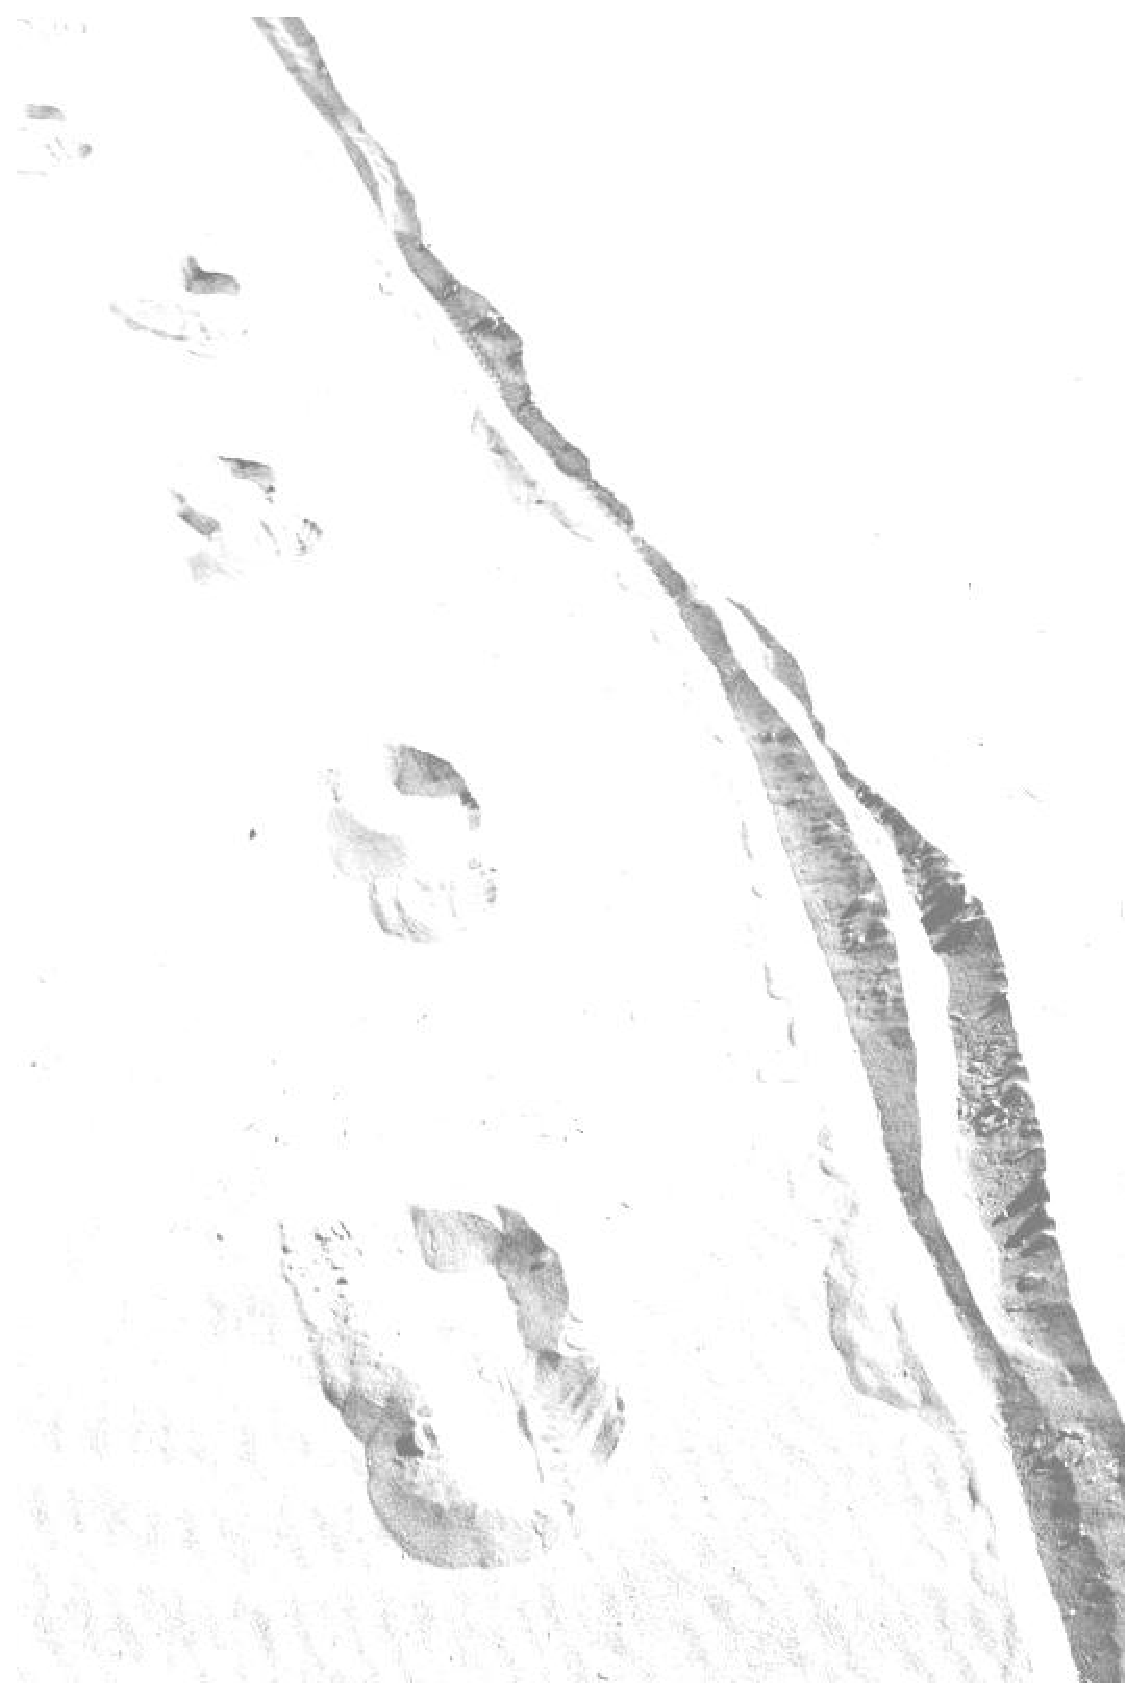
\includegraphics[width=0.55\paperwidth, height = \paperheight]{Figures/Track.eps}}}
  \begin{frame}{\normalsize Outline}
  \tableofcontents[currentsection]
  \end{frame}}
}



\title[Intro to Decisions]{Introduction to Decision-Making Theory}
\author[S. Gros]{\large Sebastien Gros}
\institute[NTNU]{Prof. \\ Department of Cybernetic \\ Faculty of Information Technology \\  NTNU}
\date[September 2025]{$1^\mathrm{st}$ AID Scientific Workshop, Trondheim}

%%%%%%%%%%%%%%%%%%%%%%%%%%%%%%%%%%%%%%%%%%%%%%%%%%%%%%%%%%%%%%%%%%%%%%%%

\begin{document}





{\usebackgroundtemplate{
 \parbox[c][\paperheight][b]{\paperwidth}{
    \flushright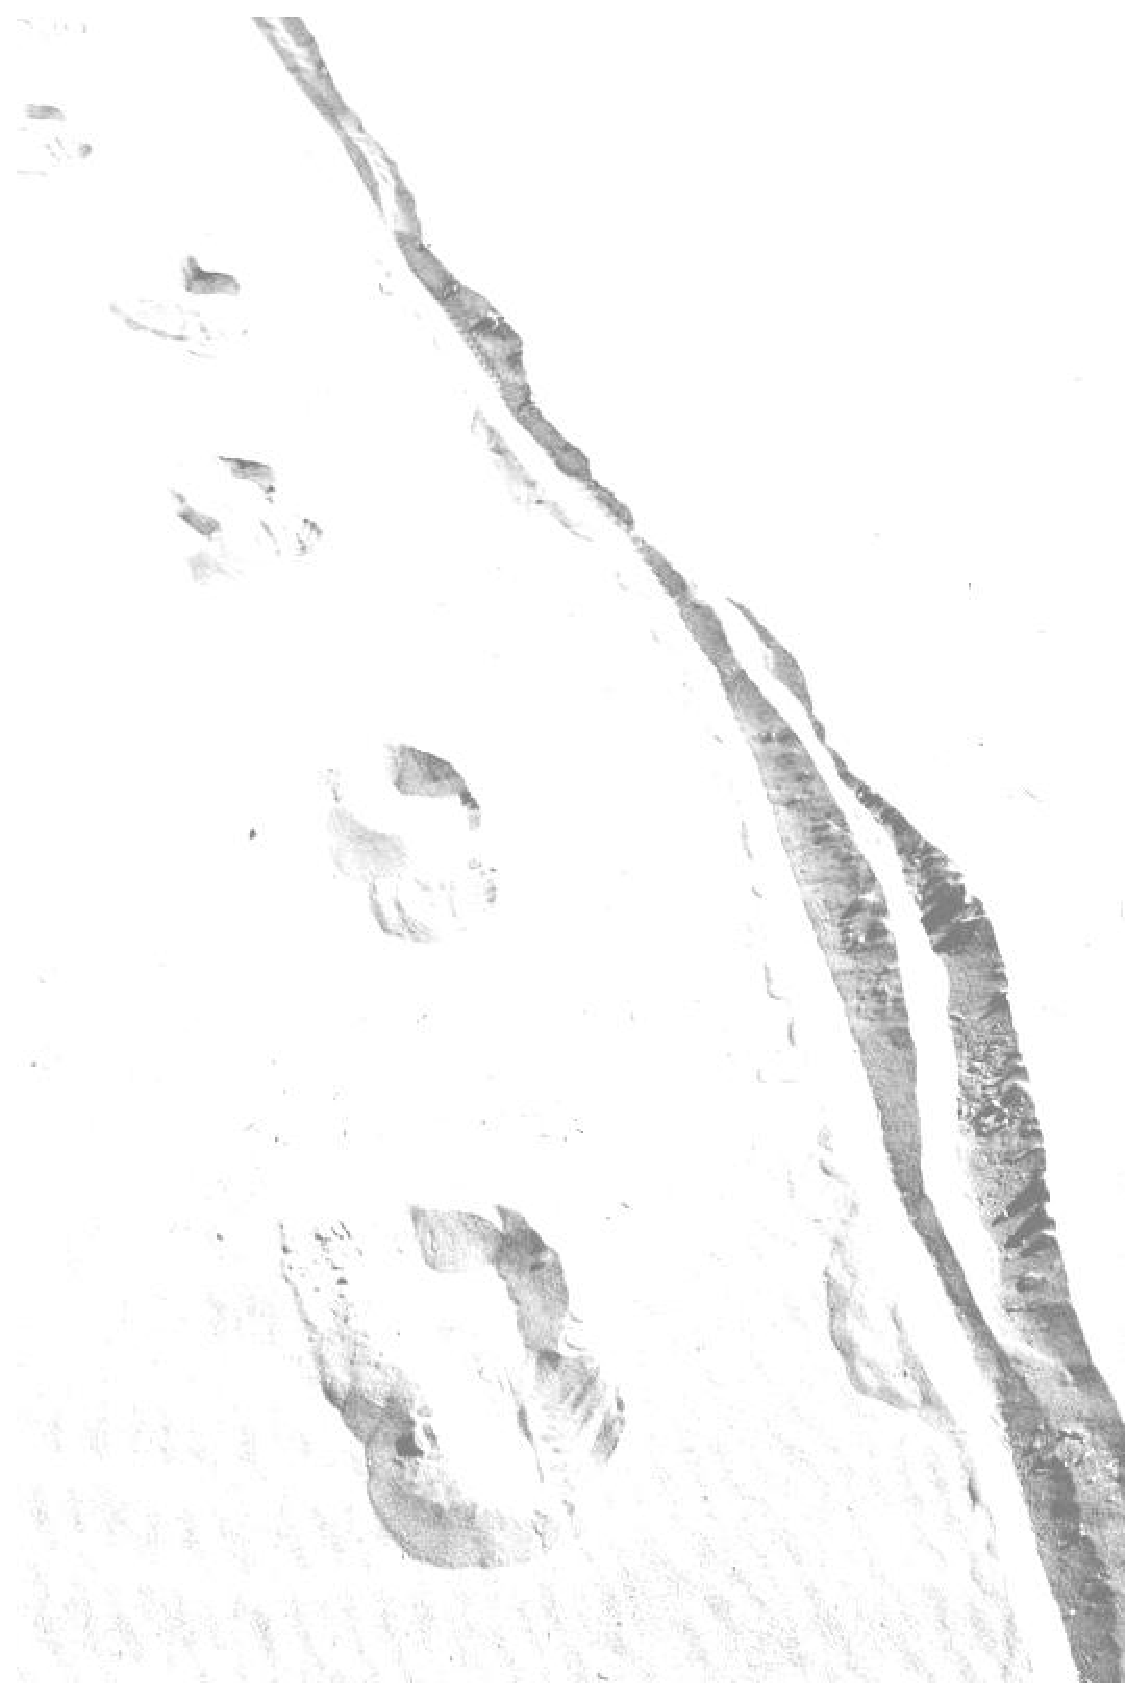
\includegraphics[width=0.55\paperwidth, height = 1\paperheight]{Figures/Track.eps}}}
\begin{frame}
\titlepage
\end{frame}}





\begin{frame}{\normalsize Forewords \& Disclaimer}
\footnotesize

\textbf{Objectives:}
\begin{itemize}
\item Put in place some common concepts \& language
\item Identify some key points in decision making (the way we mean it in AID!)
\item Paint a big (and rough) picture on the topic
\item Connect to AI
\end{itemize}
\vspace{.25cm}
\textbf{Disclaimer:} 
\begin{itemize}
\item We are a broad group who needs to get to know each others scientifically. Apologies if we don't "hit" the right level for all. \\We have favored simplicity over ``absolute" rigor. 
\item We have created a lot of new content for this workshop, it is not perfect (yet)
\end{itemize}
\vspace{1cm}
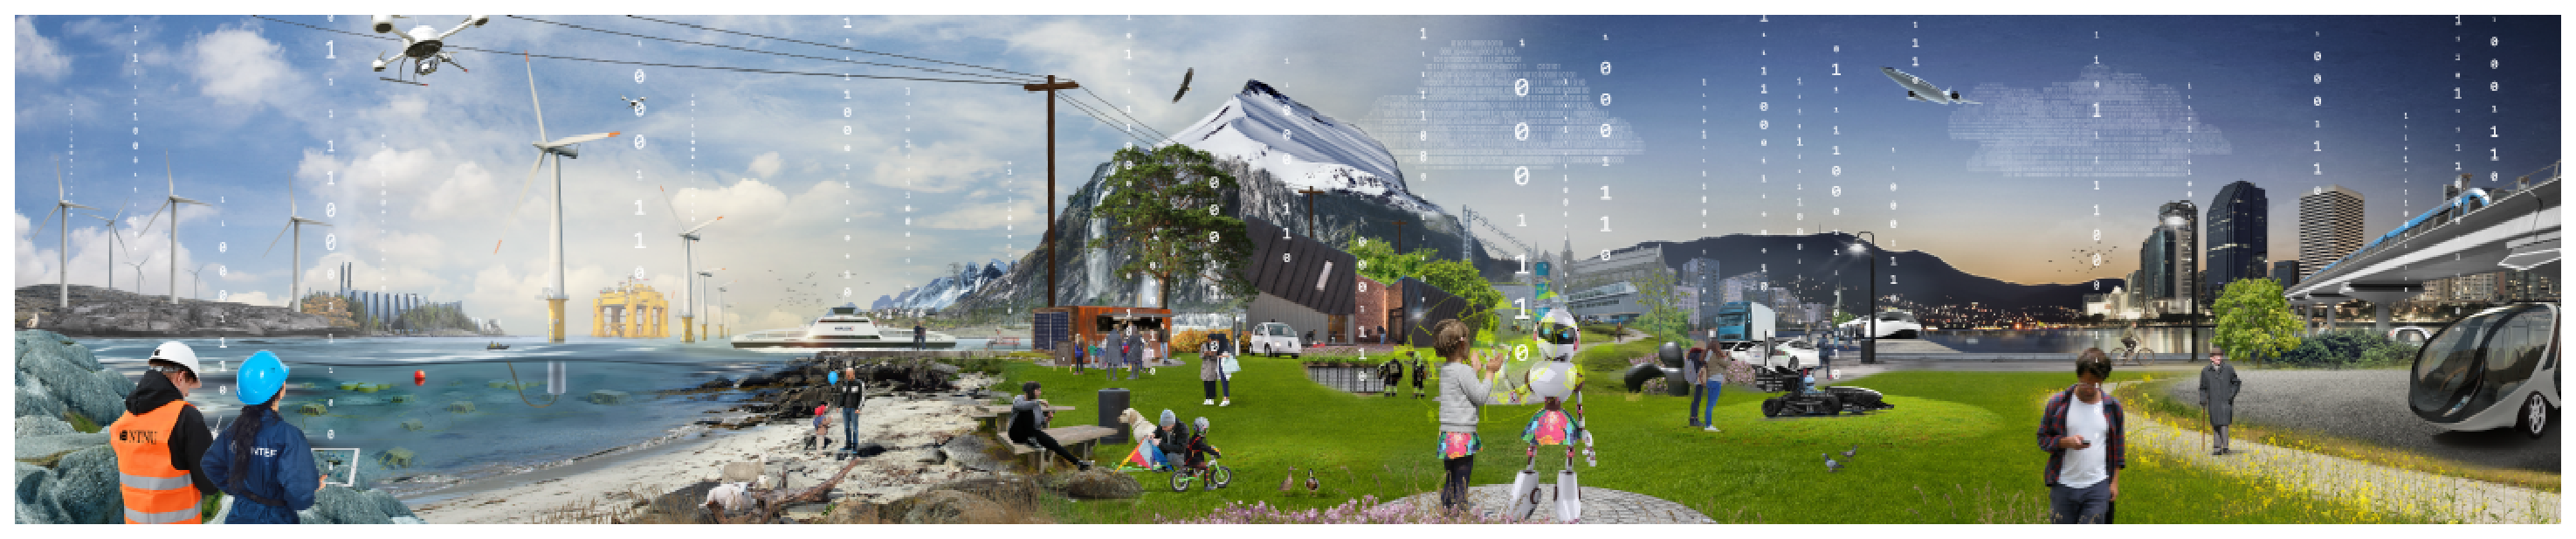
\includegraphics[width=1\textwidth,clip]{Figures/SmartGridLab.eps}

\end{frame}

\section{Some Basics of Decision Making Theory}

\begin{frame}{\normalsize AID Focuses on Operational Decisions}
\footnotesize
%\vspace{-.5cm}
\begin{center}
\textit{Layman term for ``sequential decision making"}
\end{center}
\vspace{-.2cm}
\textbf{Why focusing on operational decisions?}
\begin{itemize}
\item Decisions that we take repeatedly / ``continuously"% (e.g. balance energy production-demand)
\item Observations give us information on how good our past decisions were
\item Gives the opportunity to improve on how we take our decisions
\end{itemize}
\vspace{.25cm}
\visible<2->{
\textbf{Decision process}

\vspace{-.5cm}

\begin{columns}
\column{0.65\textwidth}

\newcommand{\Sys}{\vspace{-0.25cm}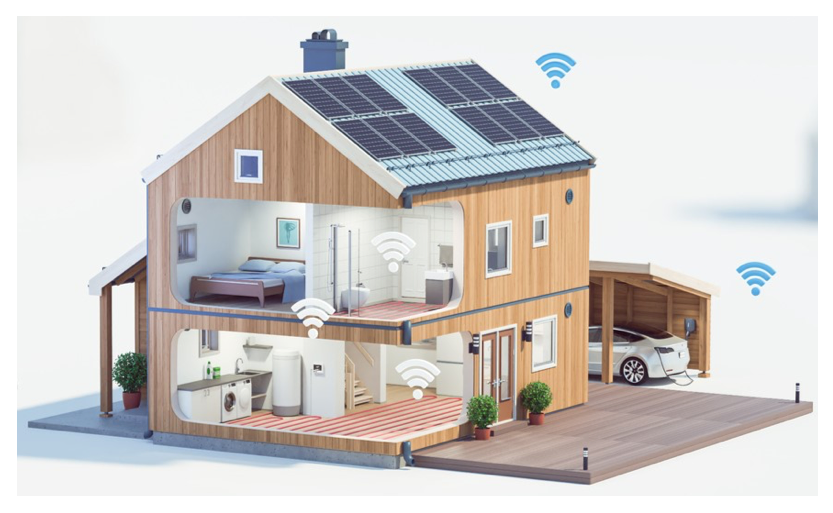
\includegraphics[width=1\textwidth,clip]{Figures/SmartHouse.eps}}

\tikzstyle{Sys_block} = [rectangle, draw, fill=none,  text width=3.cm, text centered, rounded corners, minimum height=4em,inner sep=2pt]
\tikzstyle{Opt_block} = [rectangle, draw, fill=myLightGreen,  text width=3.5cm,  text centered, rounded corners]
\tikzstyle{line} = [draw, -latex']


\begin{tikzpicture}[->,>=stealth']

\node [Sys_block] (sys0) {\Sys};


 \node [Opt_block, left of=sys0, node distance = 4.4cm] (opt0) {
 \begin{minipage}[c]{3.5cm}
 \center
Information to Decisions\\
\visible<5->{\textbf{Policy} $\vect\pi$}
\end{minipage}
 };
 
 \path  (sys0) edge[bend left=20]  node[anchor=north] {Information} (opt0)
 (opt0) edge[bend left=20]  node[anchor=south] {Action} (sys0);
\end{tikzpicture}
}
\column{0.325\textwidth}
\visible<6->{
\begin{alertblock}{}
\center
Decisions are taken from current information, knowing that the future is uncertain, and that more information will be available for subsequent decisions
\end{alertblock}}
\end{columns}


%\vspace{-0.75cm}
\begin{columns}[t]
\column{0.32\textwidth}
\visible<3->{\begin{block}{}\center
\textcolor{myBlue2}{
\textbf{Information?}}\\ \scriptsize{Anything that should influence our decisions. \\Can be a ``deep" definition! \\ More in a bit}
\end{block}
}

\column{0.32\textwidth}

\visible<4->{\begin{block}{}\center
\textcolor{myBlue2}{\textbf{Action?}}\\ \scriptsize{Decisions implemented in the real world. \\\quad \\$\neq$ actions? }
\end{block}
}

\column{0.32\textwidth}
 \visible<5->{\begin{block}{}
 \center
 \textcolor{myBlue2}{\textbf{Policy?}}\\ \scriptsize{Something that ``turns" information into decisions/actions \\More in a bit}
 \end{block}
 }
 
\end{columns}



%\vspace{-1cm}
%\begin{itemize}
%\item \textbf{Information?} \scriptsize{Anything that should influence what we do. Can be a ``deep" definition!}
%\item \textbf{Action?} \scriptsize{Decisions implemented in the real world. $\neq$ actions?}
%\item \visible<4->{\textbf{Policy?} \scriptsize{Something that ``turns" information into decisions/actions. More in a bit.}}
%\end{itemize}

%\end{columns}

\end{frame}


\begin{frame}{\normalsize Examples of Operational Decisions?}
\footnotesize

\begin{columns}[t]
\column{0.65\textwidth}


\newcommand{\Sys}{\vspace{-0.25cm}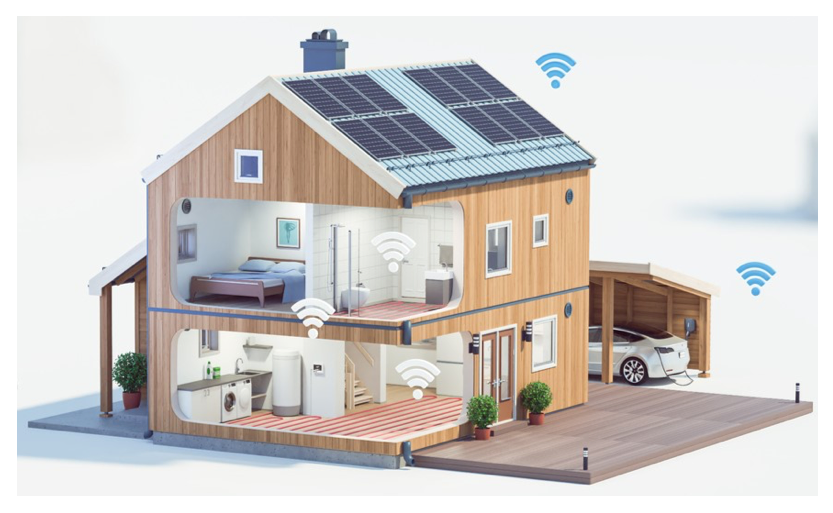
\includegraphics[width=1\textwidth,clip]{Figures/SmartHouse.eps}}

\tikzstyle{Sys_block} = [rectangle, draw, fill=none,  text width=3.cm, text centered, rounded corners, minimum height=4em,inner sep=2pt]
\tikzstyle{Opt_block} = [rectangle, draw, fill=myLightGreen,  text width=3.5cm,  text centered, rounded corners]
\tikzstyle{line} = [draw, -latex']


\begin{tikzpicture}[->,>=stealth']

\node [Sys_block] (sys0) {\Sys};


 \node [Opt_block, left of=sys0, node distance = 4.4cm] (opt0) {
 \begin{minipage}[c]{3.5cm}
 \center
Information to Decisions\\
\textbf{Policy} $\vect\pi$
\end{minipage}
 };
 
 \path  (sys0) edge[bend left=20]  node[anchor=north] {Information} (opt0)
 (opt0) edge[bend left=20]  node[anchor=south] {Action} (sys0);
\end{tikzpicture}

\column{0.325\textwidth}
\begin{alertblock}{}
\center
\textbf{Ubiquitous in our society, critical in many domains}
\end{alertblock}
\end{columns}

\begin{overlayarea}{\textwidth}{0.5\textheight}
\only<1-5>{\textbf{Energy management}:
\begin{itemize}
\item Houses \& buildings: modulate demand (heating, cooling ventilation) to facilitate supply-demand matching, reduce congestion
\item \visible<2->{Commercial surfaces: same + refrigeration, cooling}
\item\visible<3->{ Production: schedule \& adjust production, manage hydro reserve, pumped hydro, downtimes, etc.}
\item \visible<4->{Storage \& EV charging: optimize usage, demand to facilitate supply-demand matching, reduce congestion}
\item \visible<5->{Overall system: reduce the cost of uncertainty in supply-demand matching, coordinate all assets}
\end{itemize}
}
\only<6-8>{\textbf{Healthcare}:
\begin{itemize}
\item Clinical pathways: how to navigate a patient through a hospital, decide where to go next and when?
\item \visible<7-> {Personalized medicine: decide on how to adjust treatments to each patient, leverage health digitalization, wearables, schedule human intervention}
\item\visible<8->{Optimize medical acts: automate decisions, involve doctors when and where they are needed}
\end{itemize}
}
%\only<9>{\textbf{Processes}:
%\begin{itemize}
%\item Chemical \& Bioreactors: steer the process (concentrations, temperatures, mixing)
%\item \visible<7-> {Personalized medicine: decide on how to adjust treatments to each patient, leverage health digitalization, wearables, schedule human intervention}
%\item\visible<8->{Optimize medical acts: automate decisions, involve doctors when and where they are needed}
%\end{itemize}
%}
\end{overlayarea}

%\begin{itemize}
%\item Energy management: house, building, businesses, production, transmission, distribution  
%\item Healthcare: clinical pathways, personalized medicine, treatments, etc.
%\item Processes: production quality, resource utilization, waste, regulations
%\item Logistics:   
%\end{itemize}


\end{frame}


\begin{frame}{\normalsize What is a good decision?}
\footnotesize
\vspace{.2cm}

\newcommand{\Sys}{\vspace{-0.25cm}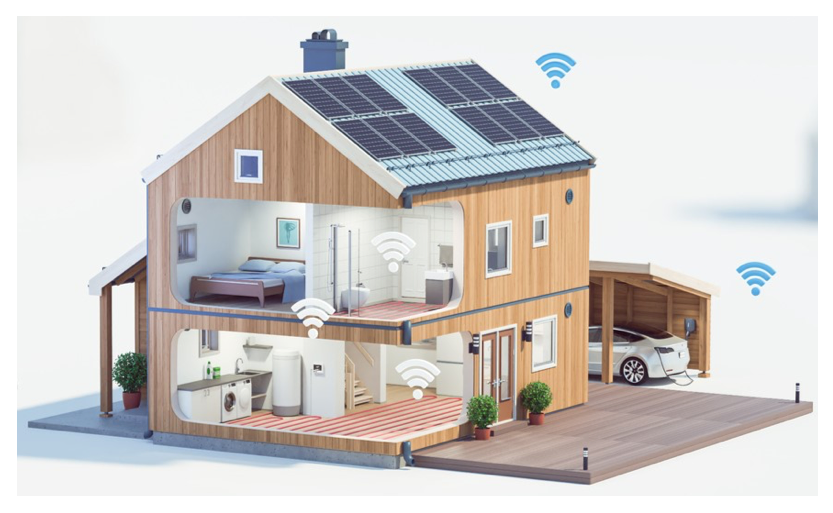
\includegraphics[width=1\textwidth,clip]{Figures/SmartHouse.eps}}

\tikzstyle{Sys_block} = [rectangle, draw, fill=none,  text width=3.cm, text centered, rounded corners, minimum height=4em,inner sep=2pt]
\tikzstyle{Opt_block} = [rectangle, draw, fill=myLightGreen,  text width=3.5cm,  text centered, rounded corners]
\tikzstyle{Util_block} = [rectangle, draw, fill=myLightBlue,  text width=3.5cm,  text centered, rounded corners]
\tikzstyle{Const_block} = [rectangle, draw, fill=myLightRed,  text width=3.5cm,  text centered, rounded corners]
\tikzstyle{line} = [draw, -latex']


\begin{tikzpicture}[->,>=stealth']

\node [Sys_block] (sys0) {\Sys};


 \node [Opt_block, left of=sys0, node distance = 5cm] (opt0) {
 \begin{minipage}[c]{3.5cm}
 \center
Information to Decisions\\
\textbf{Policy} $\vect\pi$
\end{minipage}
 };
 
 \visible<2->{
  \node [Util_block, below of=opt0, node distance = 1.6cm] (util0) {
 \begin{minipage}[c]{3.5cm}
 \center
Utility
\end{minipage}
 };}

 \visible<4->{
  \node [Const_block, above of=opt0, node distance = 1.6cm] (limit0) {
 \begin{minipage}[c]{3.5cm}
 \center
Constraints
\end{minipage}
 };
}
 
 \path  (sys0) edge[bend left=20]  node[anchor=north] {Information} (opt0)
 (opt0) edge[bend left=20]  node[anchor=south] {Action} (sys0);
  \visible<2->{ \path (util0) edge[<->]  node[anchor=east] {Performance} (opt0);}
  \visible<4->{ \path (limit0) edge[<->]  node[anchor=east] {Violations} (opt0);}
 
\end{tikzpicture}


\begin{columns}[t]
\column{0.55\textwidth}

\begin{overlayarea}{\textwidth}{0.5\textheight}
\only<2>{
\vspace{-0.5cm}
\begin{block}{}
\textbf{Utility?}
\begin{itemize}
\scriptsize
%\item ``Grades" our current situation 
\item (Info, Action) $\mapsto$ ``summable grade"\\ \begin{tiny}(e.g. real number)\end{tiny}
\item Allows for comparing policies
\item We want the highest ``average grade" possible \begin{tiny}(more on that later)\end{tiny} 
\item Utility is Instantaneous, policy looks at long-term performance 
\end{itemize}
\end{block}
}
\only<3->{
\textbf{Utility?} Examples
\begin{itemize}
\scriptsize
\item Economic revenue (or negative cost)
\item Comfort
\item Quality of service
\item Equity (e.g. Gini coeff?)
\item etc...
\end{itemize}
\qquad\qquad\qquad \textit{\scriptsize may be hard to quantify!} 
}
\end{overlayarea}



\column{0.45\textwidth}

\begin{overlayarea}{\textwidth}{0.5\textheight}
\only<4>{
\vspace{-0.5cm}
\begin{block}{}
\textbf{Constraints?}
\begin{itemize}
\scriptsize
\item Flag ``unacceptable" situations
\item (Info, Action) $\mapsto$ violation or not
\item Constraints have priority over utility
\item Violation can be ``Utility = $-\infty$" 
\item Constraints are Instantaneous, policy looks at long-term safety
\end{itemize}
\end{block}
}
\only<5->{
\textbf{Constraints?} Examples
\begin{itemize}
\scriptsize
\item Action limitations (e.g. power prod.)
\item Hard safety (e.g. max speed)
\item Minimum quality (e.g. of a product)
\item Risk (e.g. prob. of failure)
\end{itemize}
}
\end{overlayarea}


\end{columns}

\end{frame}


\begin{frame}{\normalsize Optimal Policy?}
\footnotesize

\begin{columns}[t]
\column{0.6\textwidth}

\newcommand{\Sys}{\vspace{-0.25cm}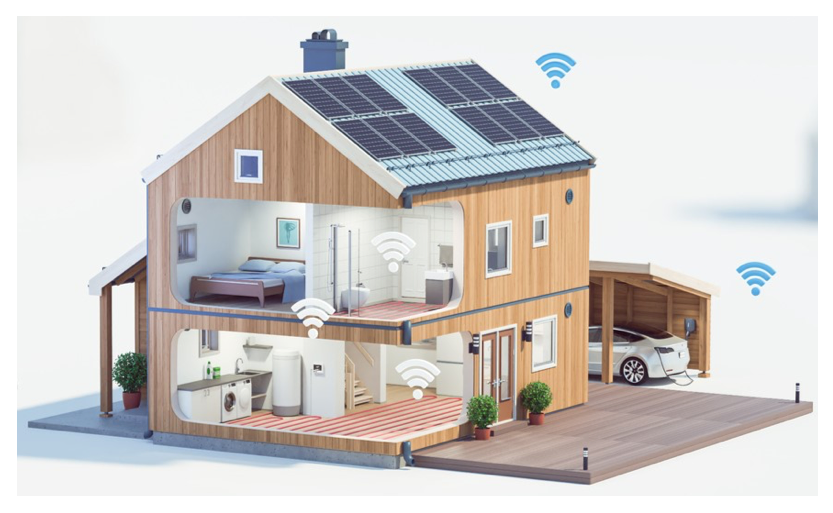
\includegraphics[width=1\textwidth,clip]{Figures/SmartHouse.eps}}

\tikzstyle{Sys_block} = [rectangle, draw, fill=none,  text width=3.cm, text centered, rounded corners, minimum height=4em,inner sep=2pt]
\tikzstyle{Opt_block} = [rectangle, draw, fill=myLightGreen,  text width=2cm,  text centered, rounded corners]
\tikzstyle{line} = [draw, -latex']


\begin{tikzpicture}[->,>=stealth']

\node [Sys_block] (sys0) {\Sys};


 \node [Opt_block, left of=sys0, node distance = 3.75cm] (opt0) {
 \begin{minipage}[c]{2cm}
 \center
\textbf{Policy} $\vect\pi$
\end{minipage}
 };
 
 \path  (sys0) edge[bend left=20]  node[anchor=north] {Information} (opt0)
 (opt0) edge[bend left=20]  node[anchor=south] {Action} (sys0);
\end{tikzpicture}


\begin{columns}[t]
\column{0.1\textwidth}

\column{0.8\textwidth}

\begin{alertblock}{}
\vspace{-.25cm}
\begin{align*}
\vect\pi^\star = \argmax_{\vect\pi}&\quad \sum_{\text{time}} \text{Utility}\\
\mathrm{s.t.}&\quad \text{Constraints ok at all time}
\end{align*}
\end{alertblock}
\column{0.1\textwidth}
\end{columns}

\vspace{.25cm}
%\textbf{Example}:
%\begin{itemize}
%\item Minimize my monthly cost of energy (sum of hourly cost)
%\item Stay within my comfort boundaries 
%\end{itemize}
\visible<13->{
\textbf{Remarks}:
\begin{itemize}
\item Policy has a ``long-term" perspective, i.e. it accounts for long-term consequences
\item Optimization is not an action but a ``map" \\info $\rightarrow$ action
\item ``Optimal policy" is supposed to be ``safe" w.r.t. the constraints
\end{itemize}}
\column{0.4\textwidth}
\vspace{-1cm}\\
\visible<2->{
\scriptsize{
\textbf{Example}: heating cost
\begin{itemize}
\item action is power
\item info is temperature
\item utility is `` - power $\cdot$ spot price"
\item constraint is temp $\geq$ 21 
\end{itemize}}
\vspace{-.4cm}
\center
  \begin{overlayarea}{\textwidth}{0.8\textheight}
    \begin{figure}
      \centering
      \only<1-3>
        {%
          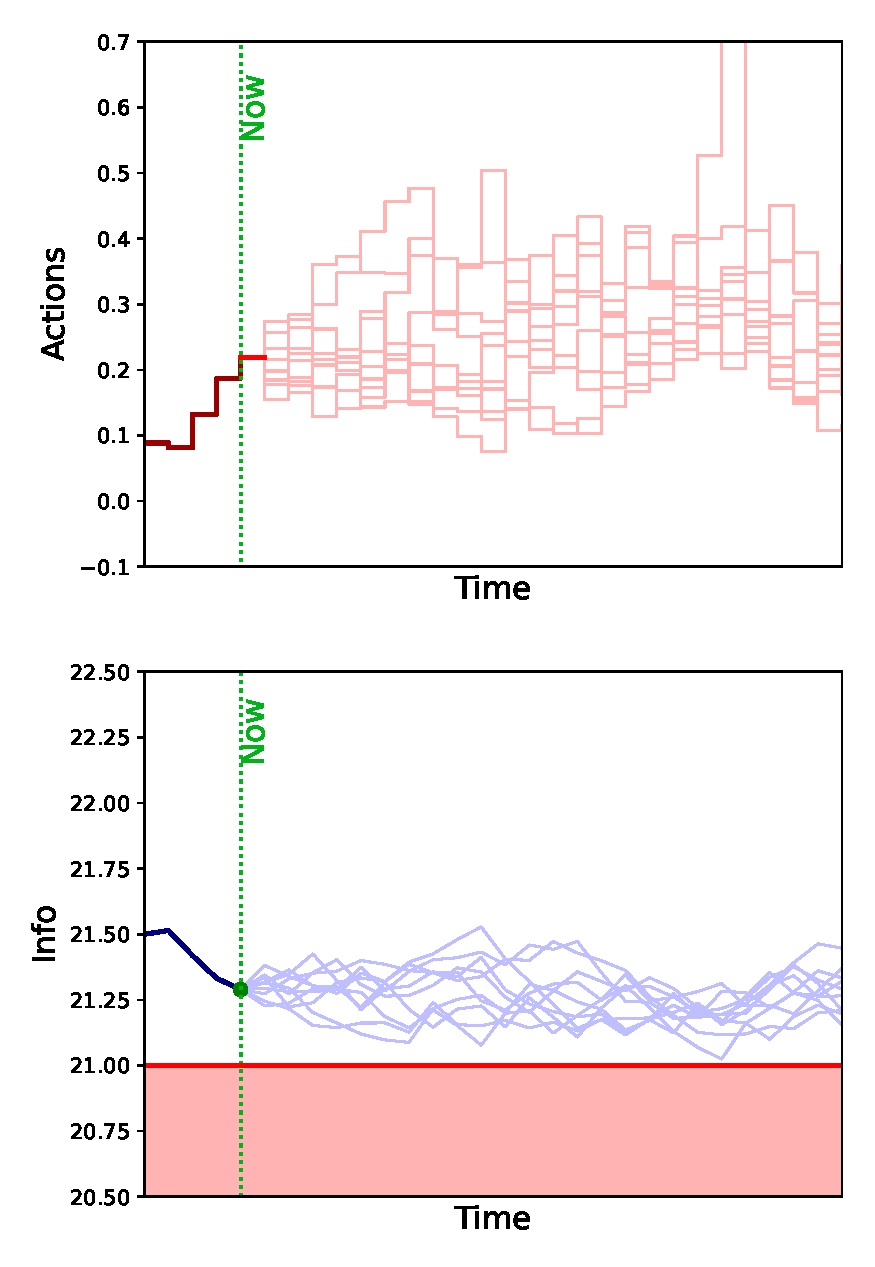
\includegraphics[width=.8\textwidth]{Codes/Basics/Policy4.eps}%
        }%
      \only<4>
        {%
          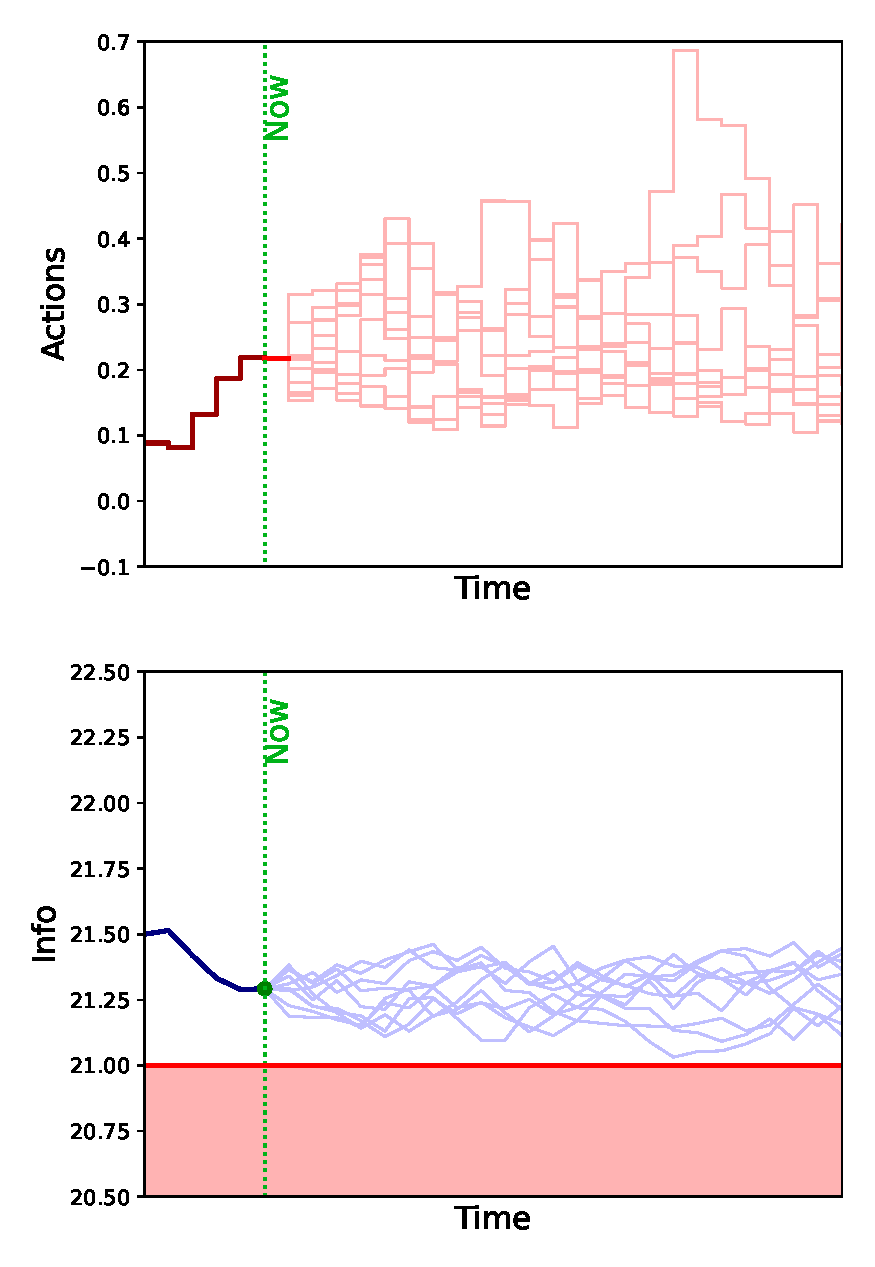
\includegraphics[width=.8\textwidth]{Codes/Basics/Policy5.eps}%
        }%
      \only<5>
        {%
          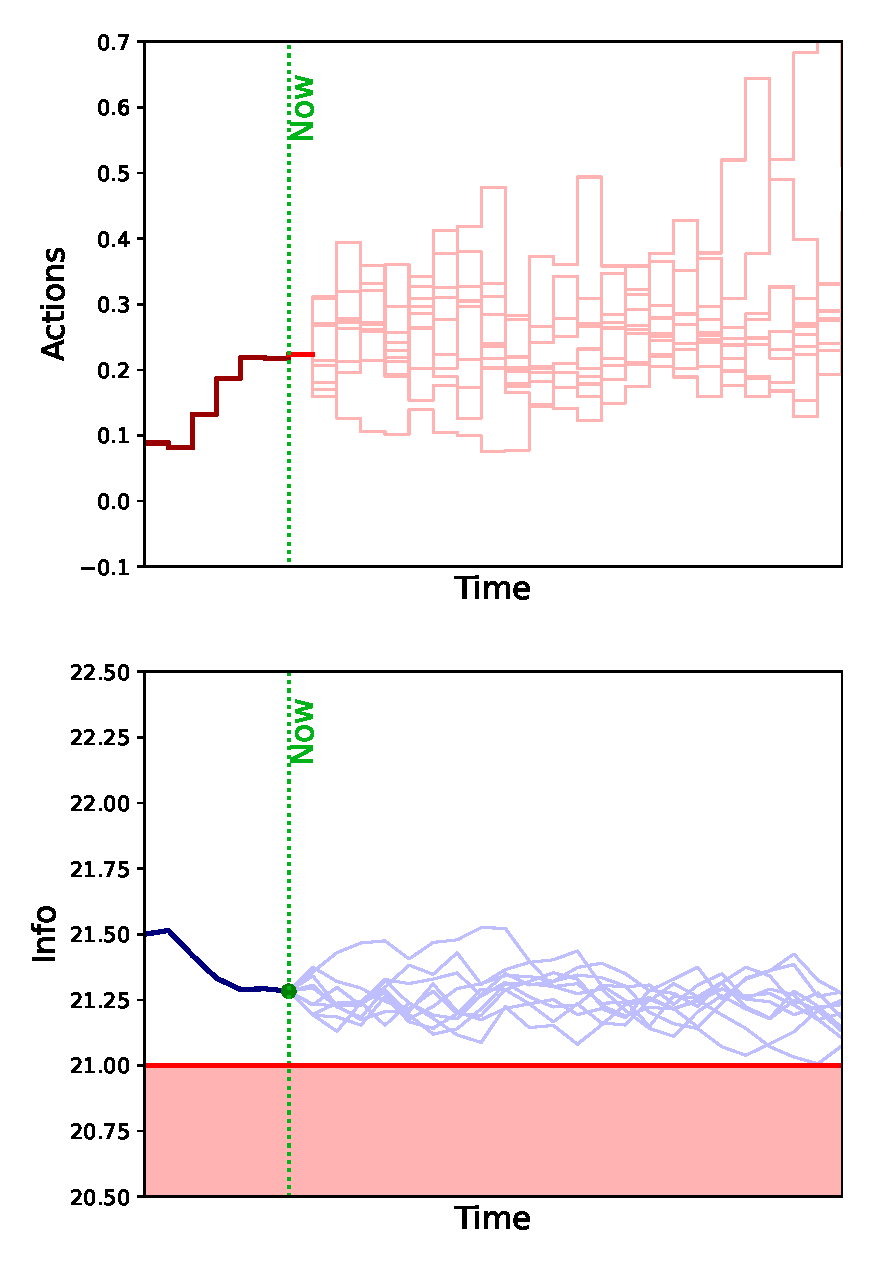
\includegraphics[width=.8\textwidth]{Codes/Basics/Policy6.eps}%
        }%
        \only<6>
        {%
          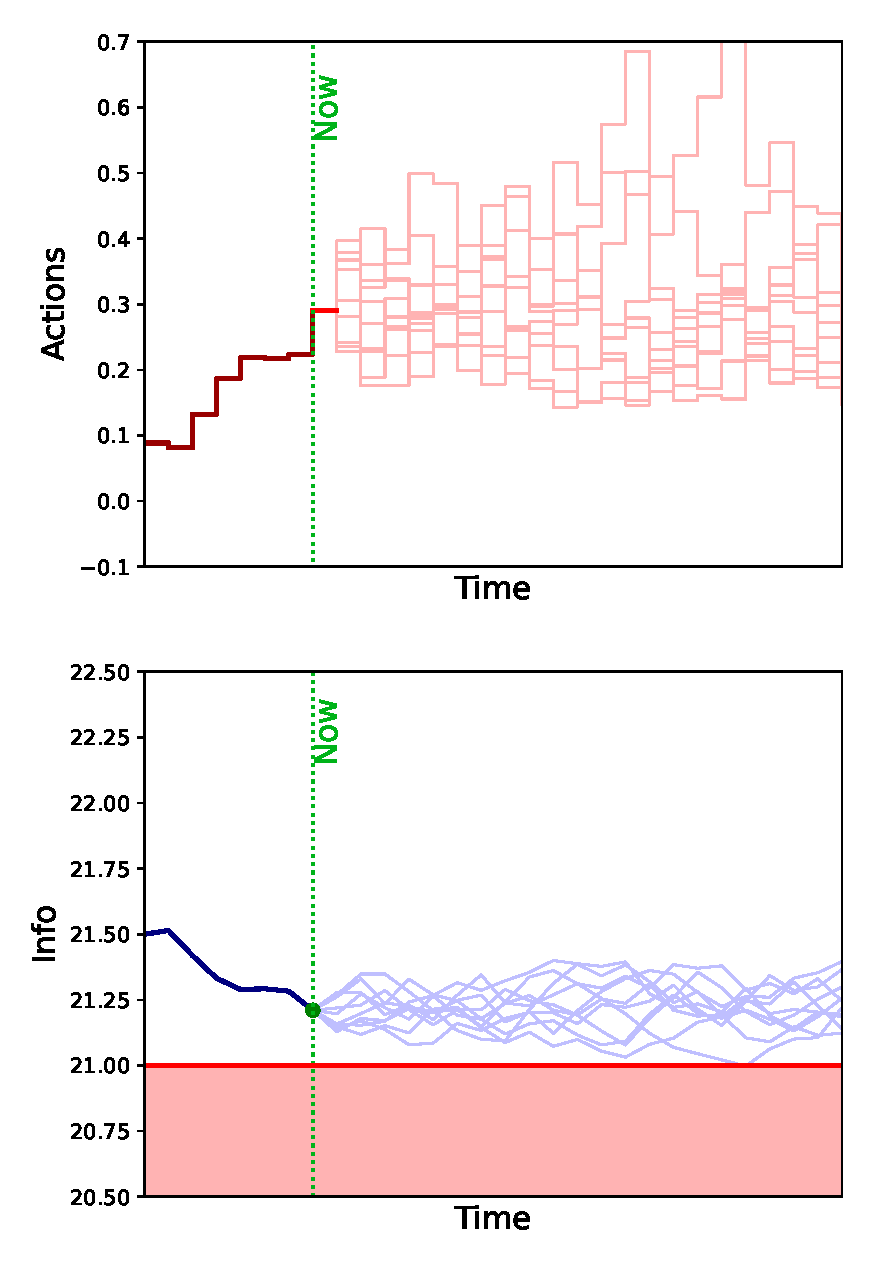
\includegraphics[width=.8\textwidth]{Codes/Basics/Policy7.eps}%
        }%
        \only<7>
        {%
          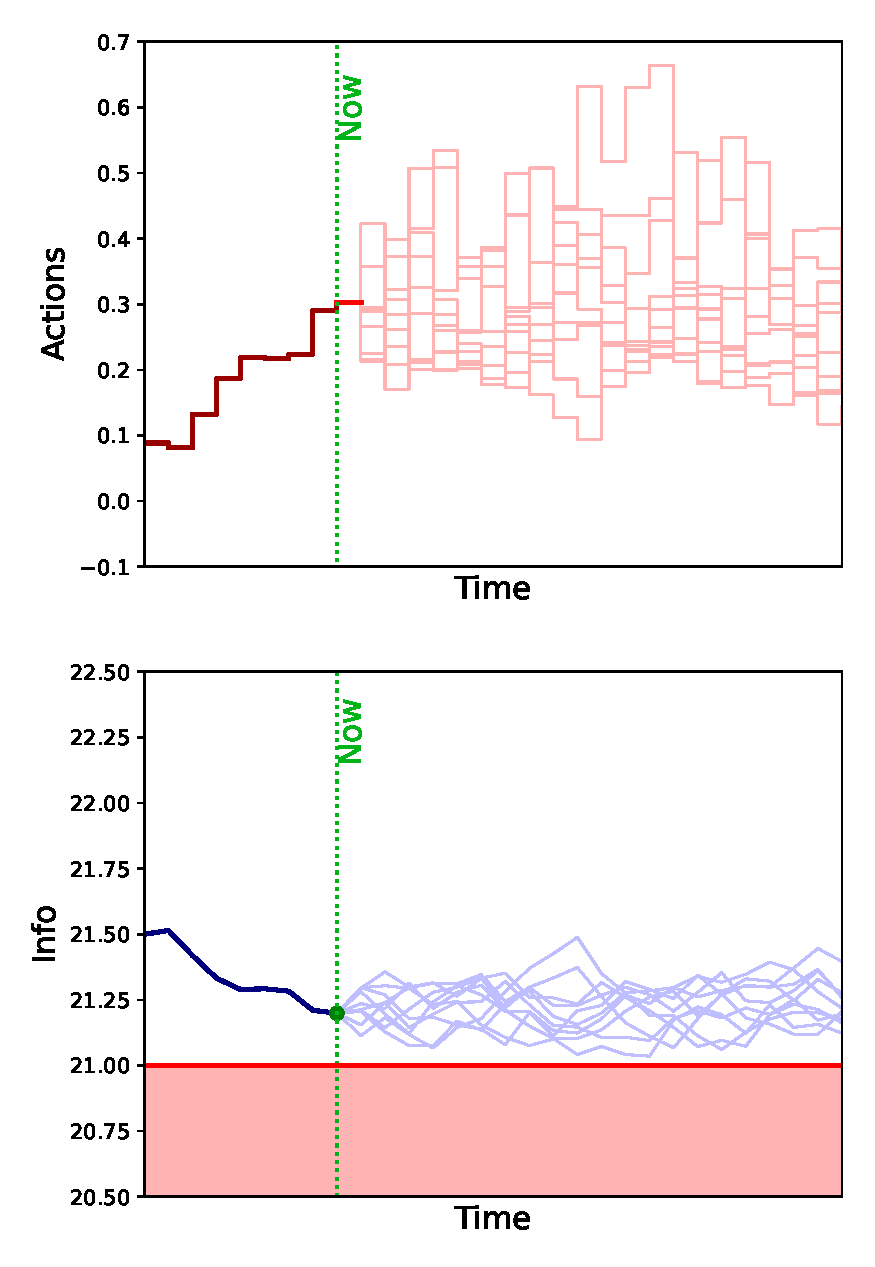
\includegraphics[width=.8\textwidth]{Codes/Basics/Policy8.eps}%
        }%
        \only<8>
        {%
          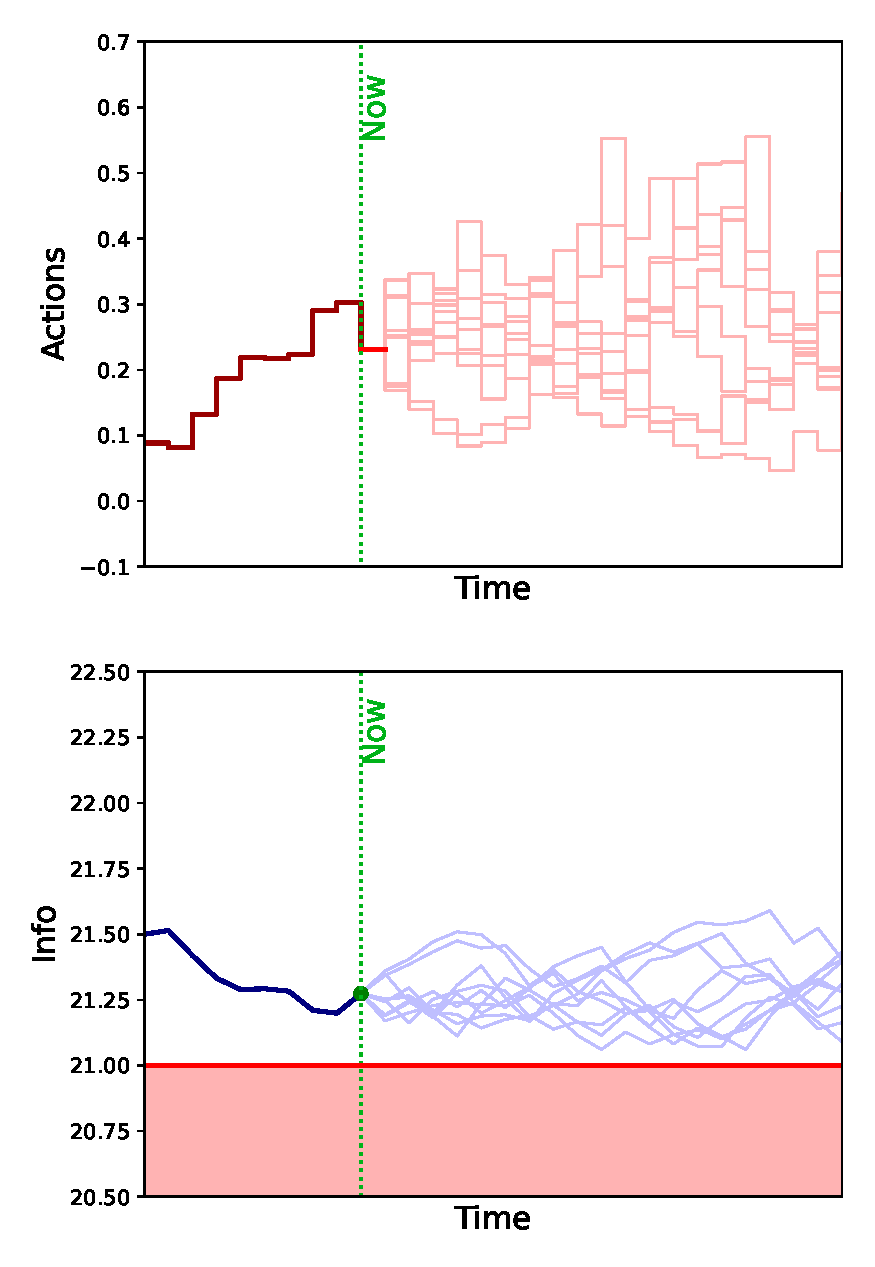
\includegraphics[width=.8\textwidth]{Codes/Basics/Policy9.eps}%
        }%
        \only<9>
        {%
          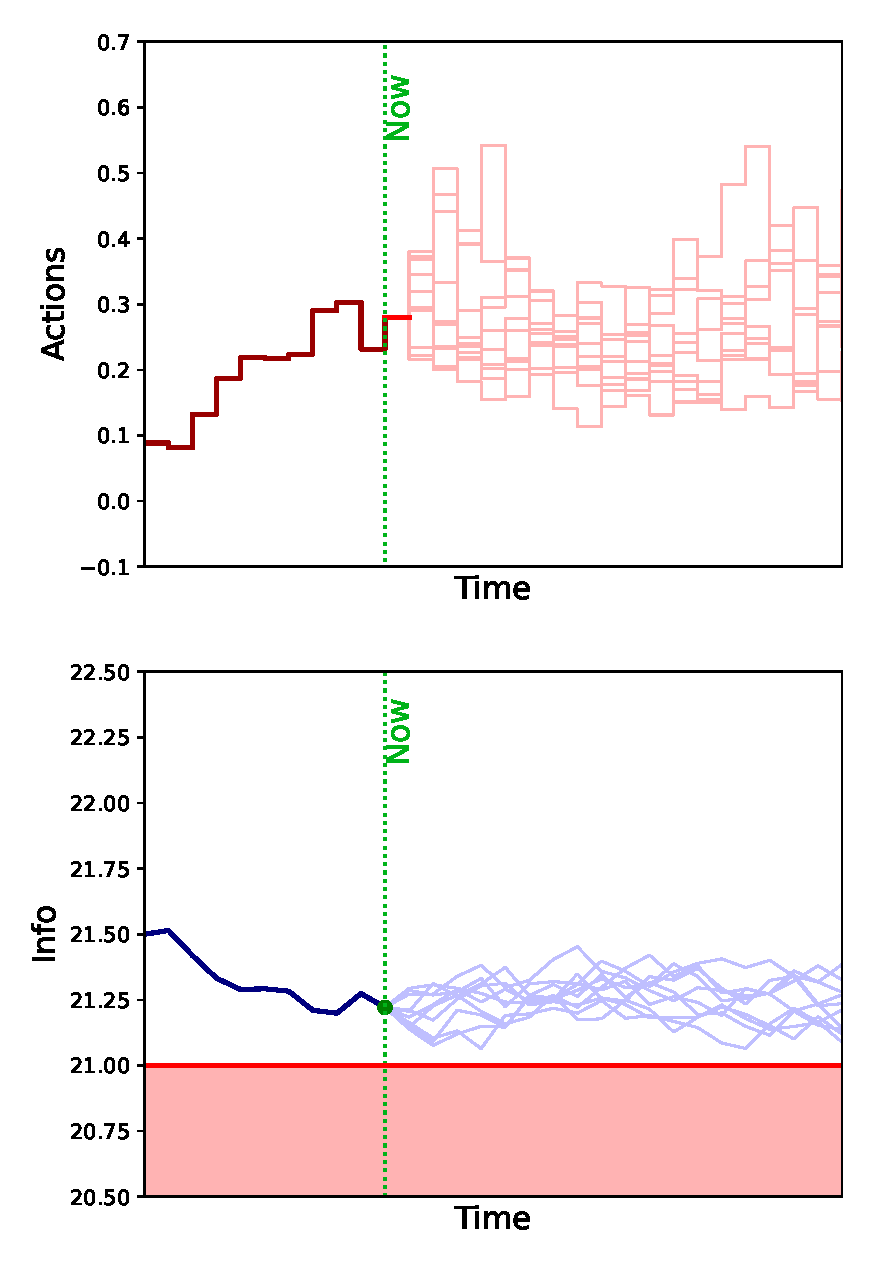
\includegraphics[width=.8\textwidth]{Codes/Basics/Policy10.eps}%
        }%
        \only<10>
        {%
          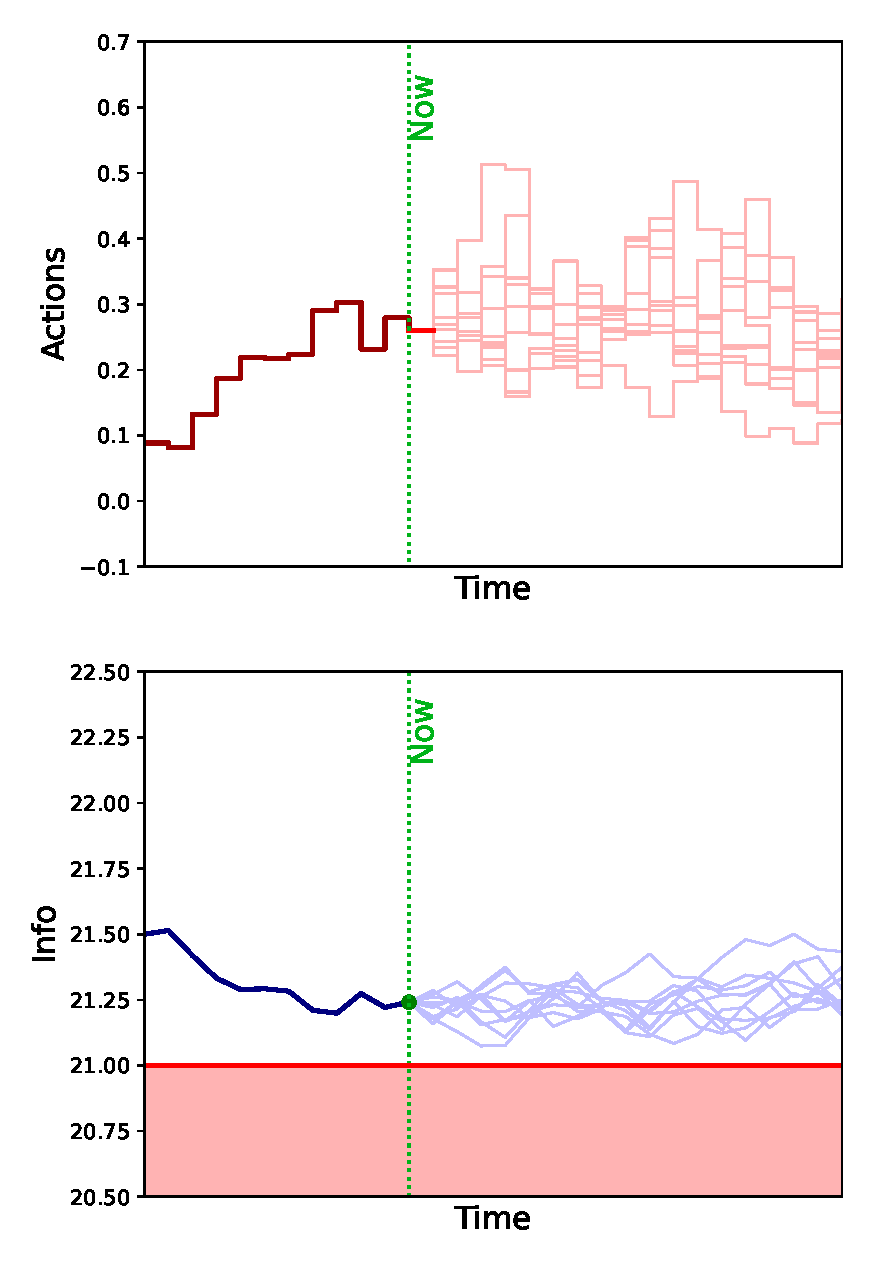
\includegraphics[width=.8\textwidth]{Codes/Basics/Policy11.eps}%
        }%
         \only<11>
        {%
          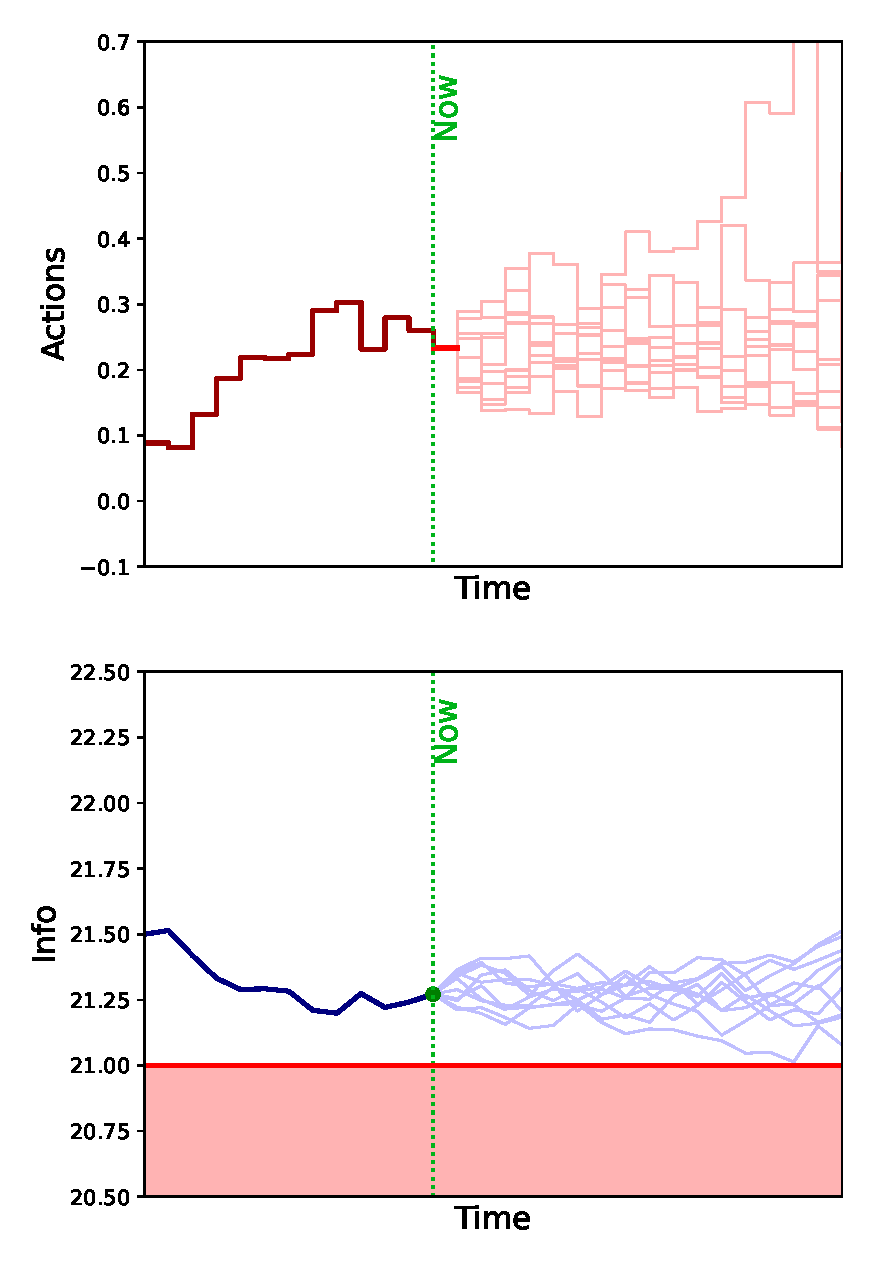
\includegraphics[width=.8\textwidth]{Codes/Basics/Policy12.eps}%
        }%
         \only<12->
        {%
          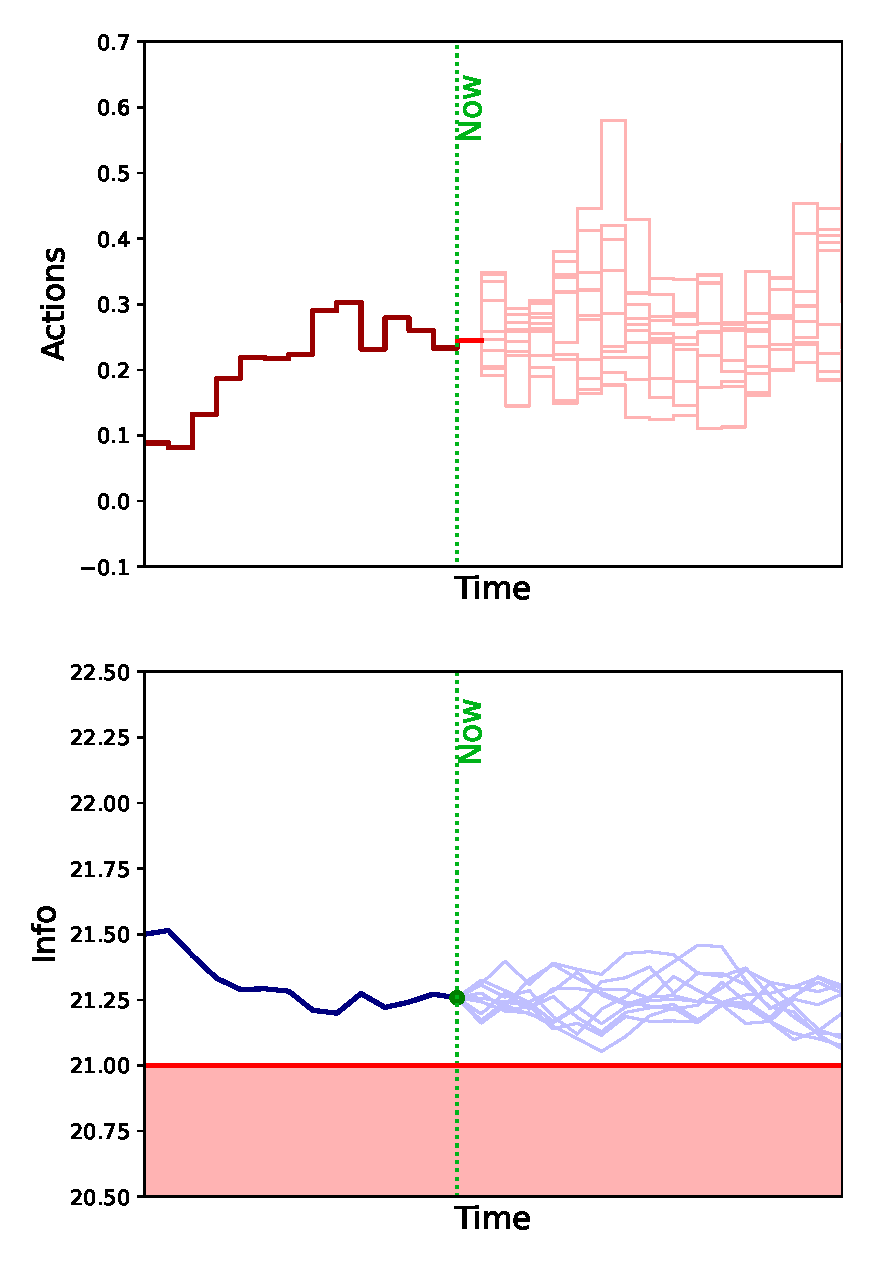
\includegraphics[width=.8\textwidth]{Codes/Basics/Policy13.eps}%
        }%
    \end{figure}
  \end{overlayarea}  }
  
  

\end{columns}



\end{frame}






\begin{frame}{\normalsize Planning vs. Decision Policy?}
\footnotesize

\begin{center}
\textcolor{myBlue2}{\textbf{Planning}}: sequence of action decided / committed over a horizon in the future
\end{center}
\vspace{.1cm}
\begin{columns}[t]
\column{0.5\textwidth}

\begin{overlayarea}{\textwidth}{0.9\textheight}
\only<2-3>{
\vspace{-.5cm}
\textbf{Example}: energy spot prices
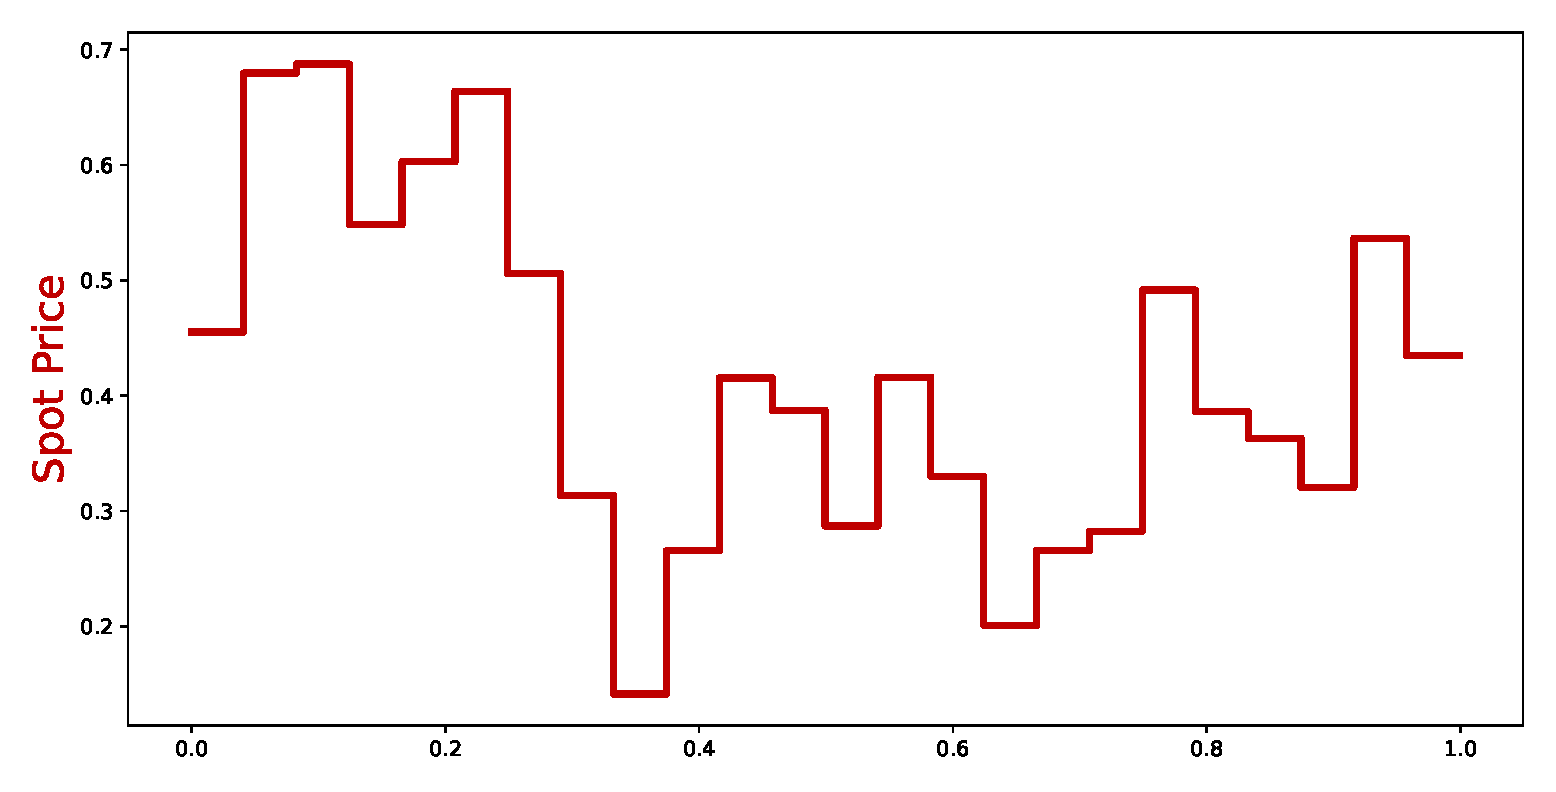
\includegraphics[width=1\textwidth,clip]{Figures/PricingAlone.eps}
\vspace{-0.5cm}
... and associated production-demand plans!\\
\vspace{0.3cm}
\visible<3->{
\begin{block}{}
\textbf{Decision-making process}
\begin{itemize}
\scriptsize
\item Actions: spot prices
\item Utility: $\sum$ participants utility
\item Constraints: 
 \begin{itemize}
\scriptsize
\item production = demand
\item prod. / transm. capacities
\end{itemize}
\end{itemize}
\vspace{-0.25cm}
\flushright \textbf{... but ``planning-style"}
\end{block}
}}
\only<4->{
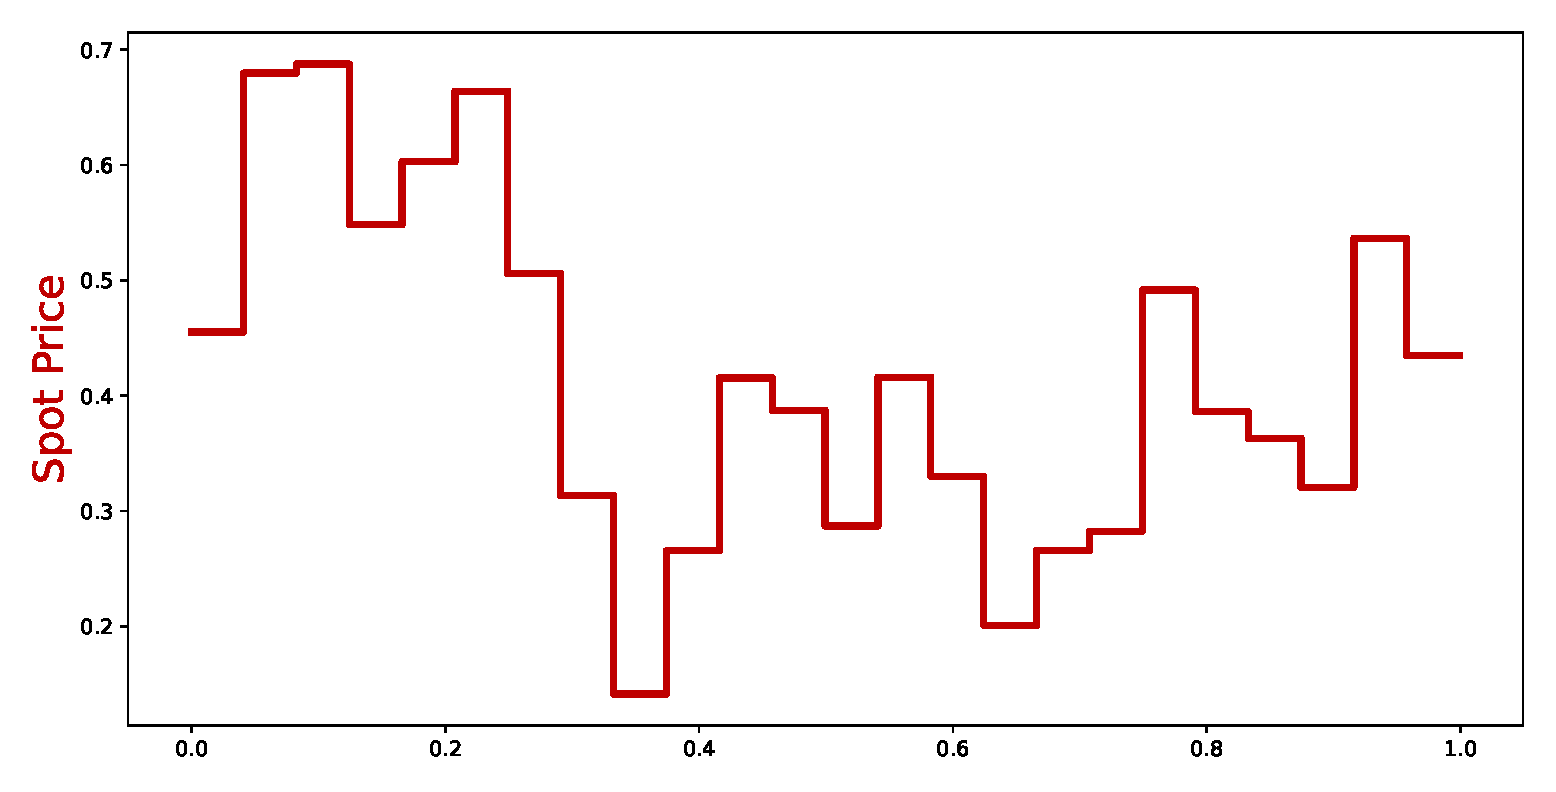
\includegraphics[width=1\textwidth,clip]{Figures/PricingAlone.eps}

\visible<7->{
\begin{block}{}
\center
\textbf{
Performance of optimal policy\\
$\geq$\\
Performance of (optimal) planning}
\end{block}
\flushright ...but planning is sometimes needed for practical reasons
}
\visible<8->{
\begin{alertblock}{}
\center
The distinction planning-policy is not obvious, but we won't expand today
\end{alertblock}
}
}
\end{overlayarea}


\column{0.5\textwidth}
\visible<4->{
\begin{alertblock}{}
\textbf{Difference with a policy?}
\begin{itemize}
\scriptsize
\item A decision policy commits only the current action, later ones not
\item Uses the latest information to establish each decision
\end{itemize}
\visible<5->{
\flushright\scriptsize{\textit{Why is a policy a good thing?}}}
\end{alertblock}

\begin{columns}
\column{0.5\textwidth}



\newcommand{\Sys}{\vspace{-0.25cm}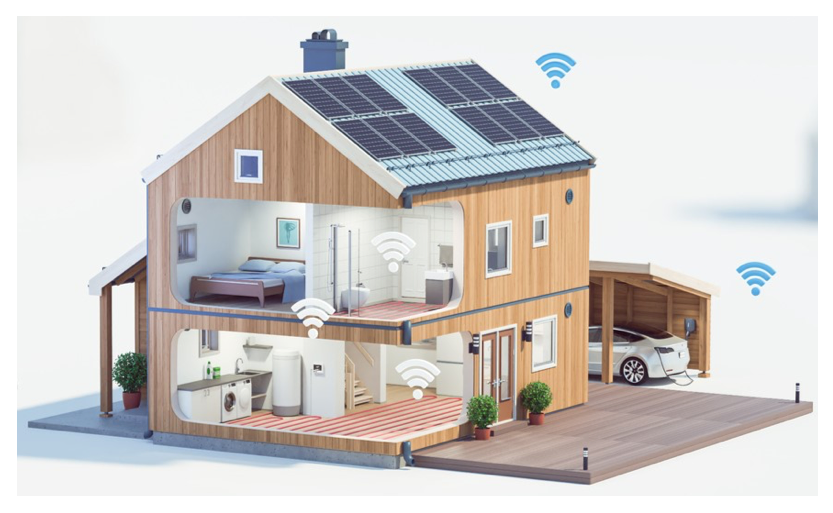
\includegraphics[width=1\textwidth,clip]{Figures/SmartHouse.eps}}

\tikzstyle{Sys_block} = [rectangle, draw, fill=none,  text width=2.cm, text centered, rounded corners, minimum height=4em,inner sep=2pt]
\tikzstyle{Opt_block} = [rectangle, draw, fill=myLightGreen,  text width=2cm,  text centered, rounded corners]
\tikzstyle{line} = [draw, -latex']


\begin{tikzpicture}[->,>=stealth']

\node [Sys_block] (sys0) {\Sys};


 \node [Opt_block, below of=sys0, node distance = 2cm] (opt0) {
 \begin{minipage}[c]{2cm}
 \center
\textbf{Policy} $\vect\pi$
\end{minipage}
 };
 
 \path  (sys0) edge[bend left=20]  node[anchor=west] {Info} (opt0)
 (opt0) edge[bend left=20]  node[anchor=east] {Action} (sys0);
\end{tikzpicture}
}
\column{0.5\textwidth}
\visible<6->{
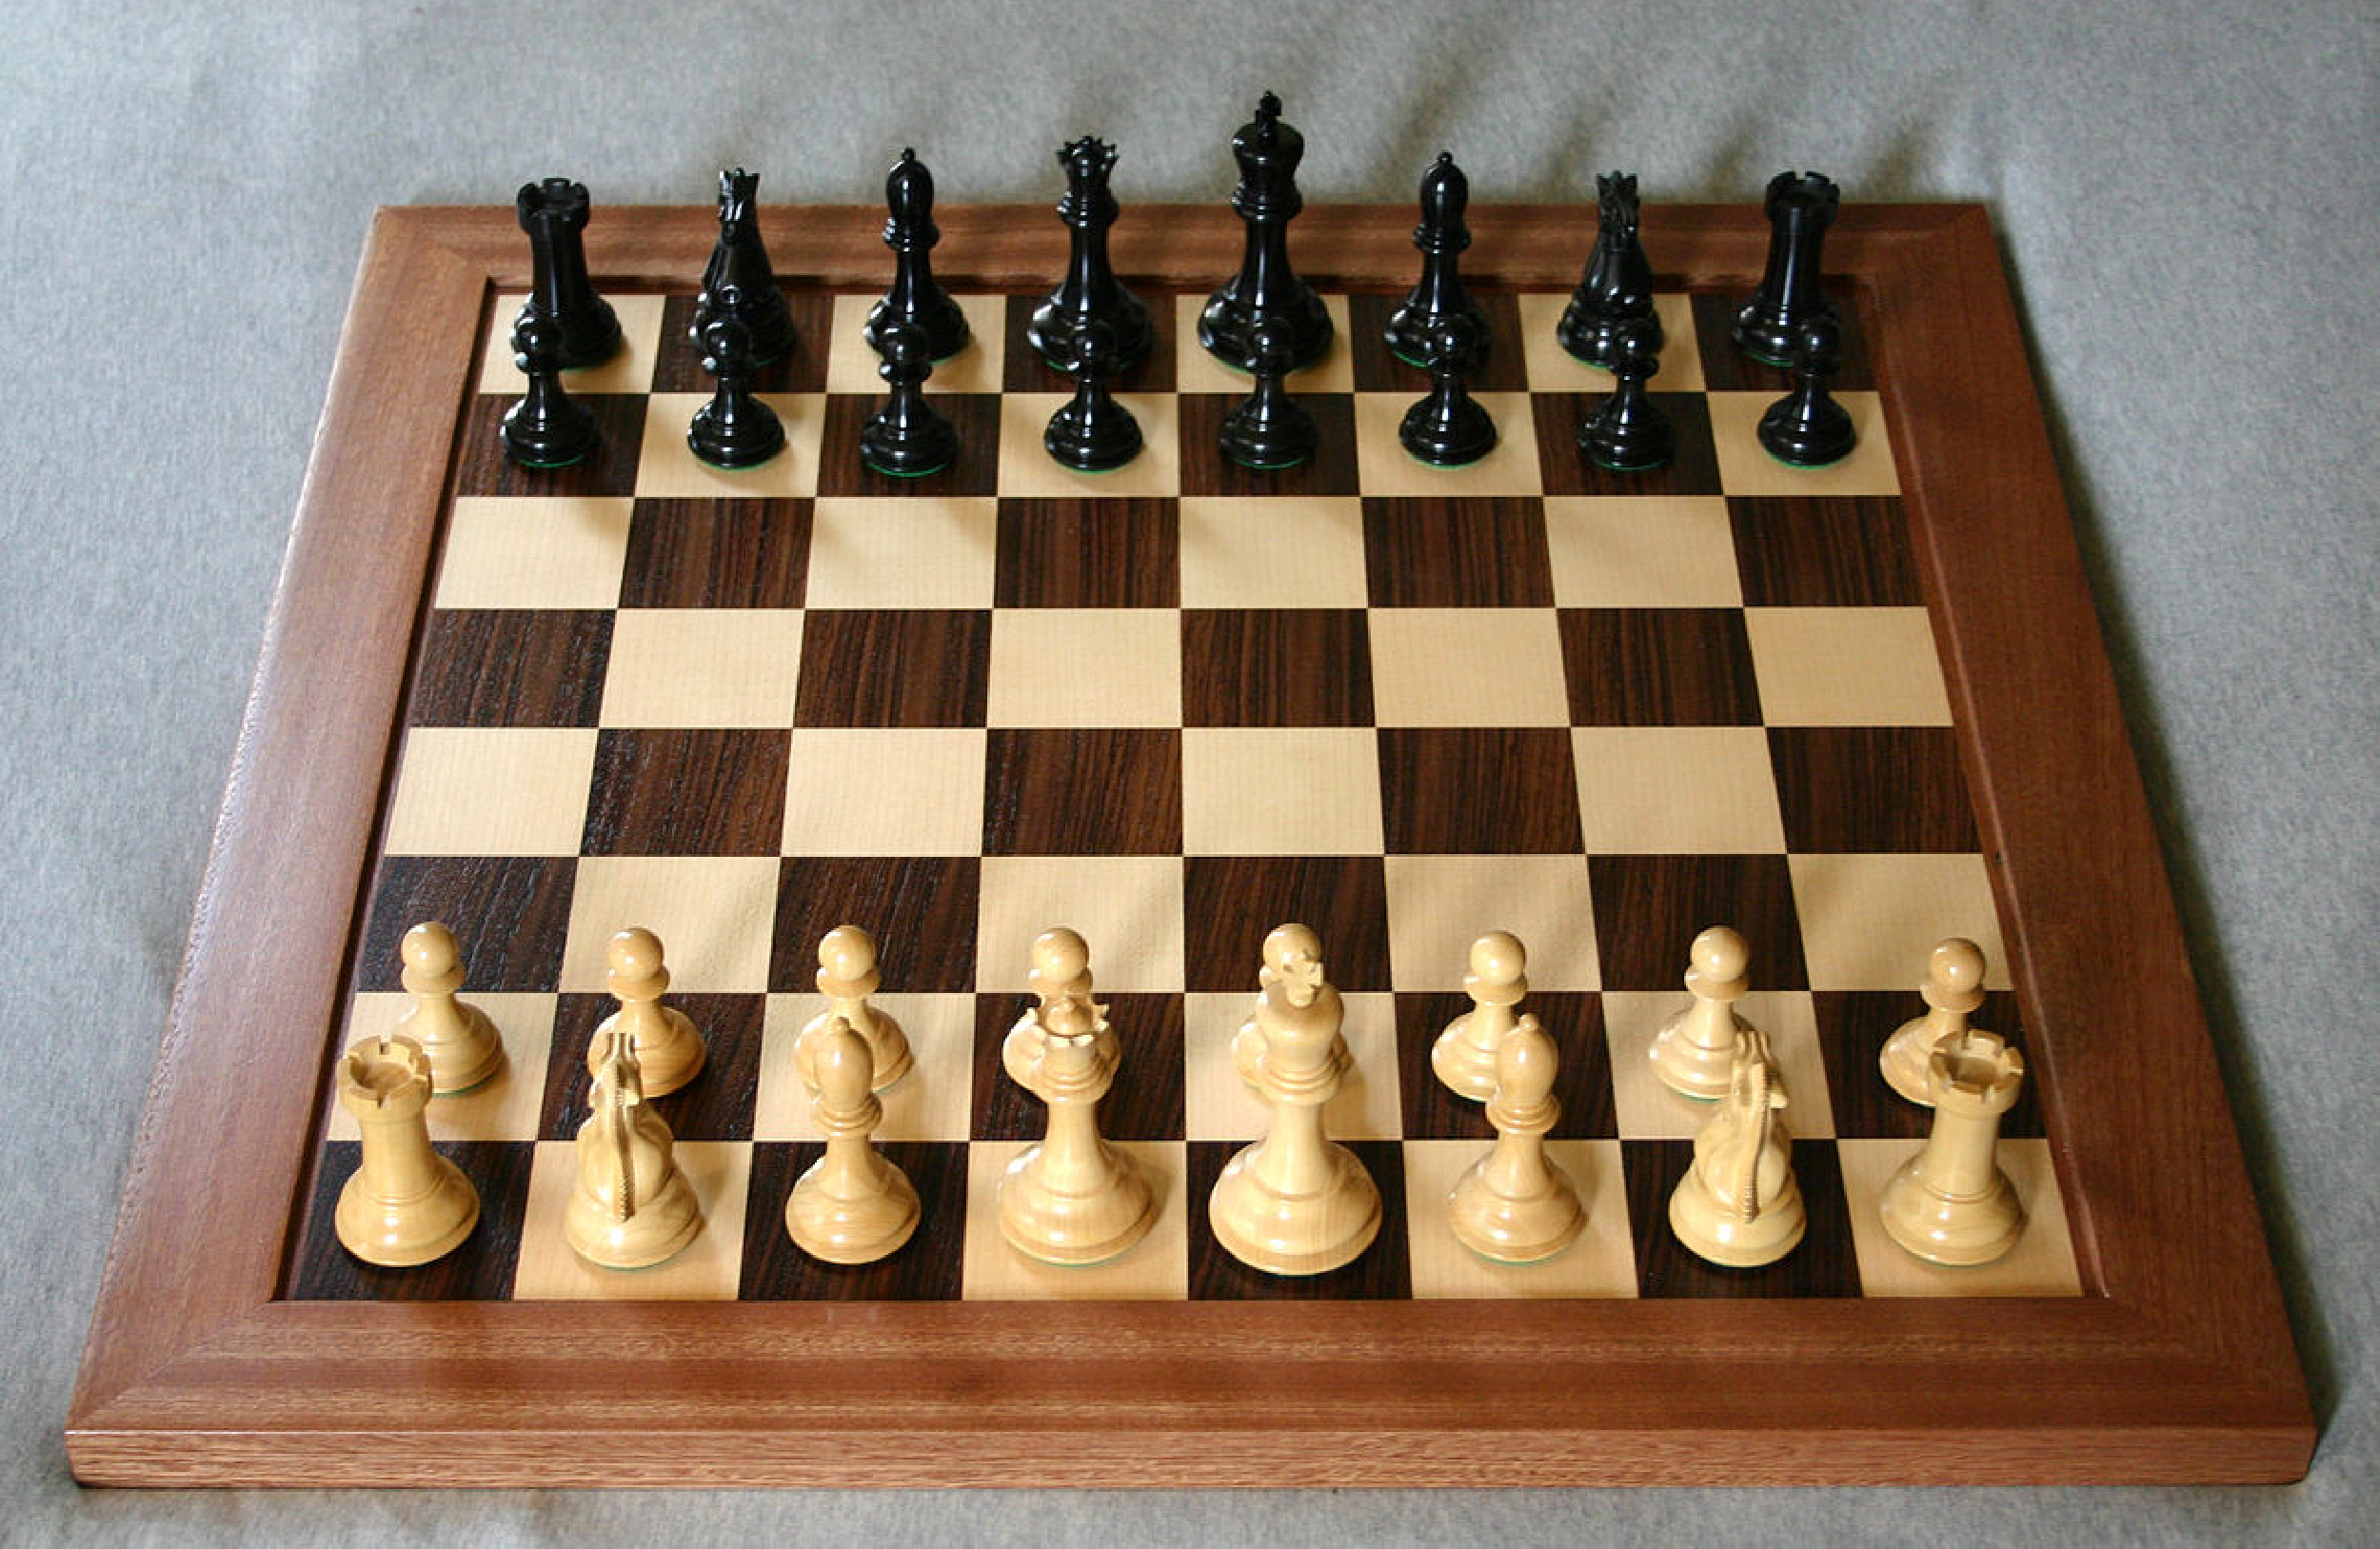
\includegraphics[width=1\textwidth,clip]{Figures/Chess.eps}}
\end{columns}

\end{columns}


\end{frame}

\begin{frame}{\normalsize Policies from Repeated Planning}
\footnotesize

\begin{columns}
\column{0.4\textwidth}



  \begin{overlayarea}{\textwidth}{0.9\textheight}
    \begin{figure}
    \newcommand{\FS}{1}
      \centering
      \only<1>
        {%
         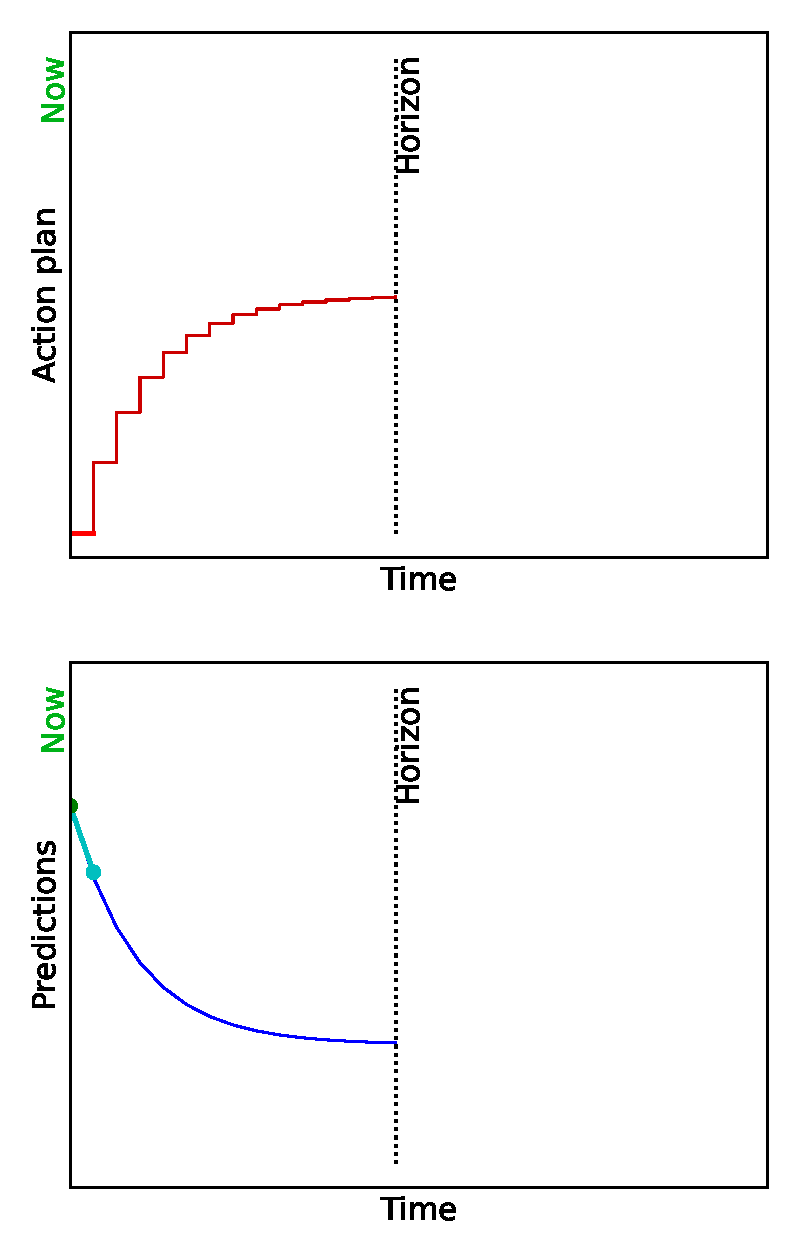
\includegraphics[width=\FS\textwidth,clip]{Codes/MPC/MPC0.eps}
        }%
              \only<2>
        {%
         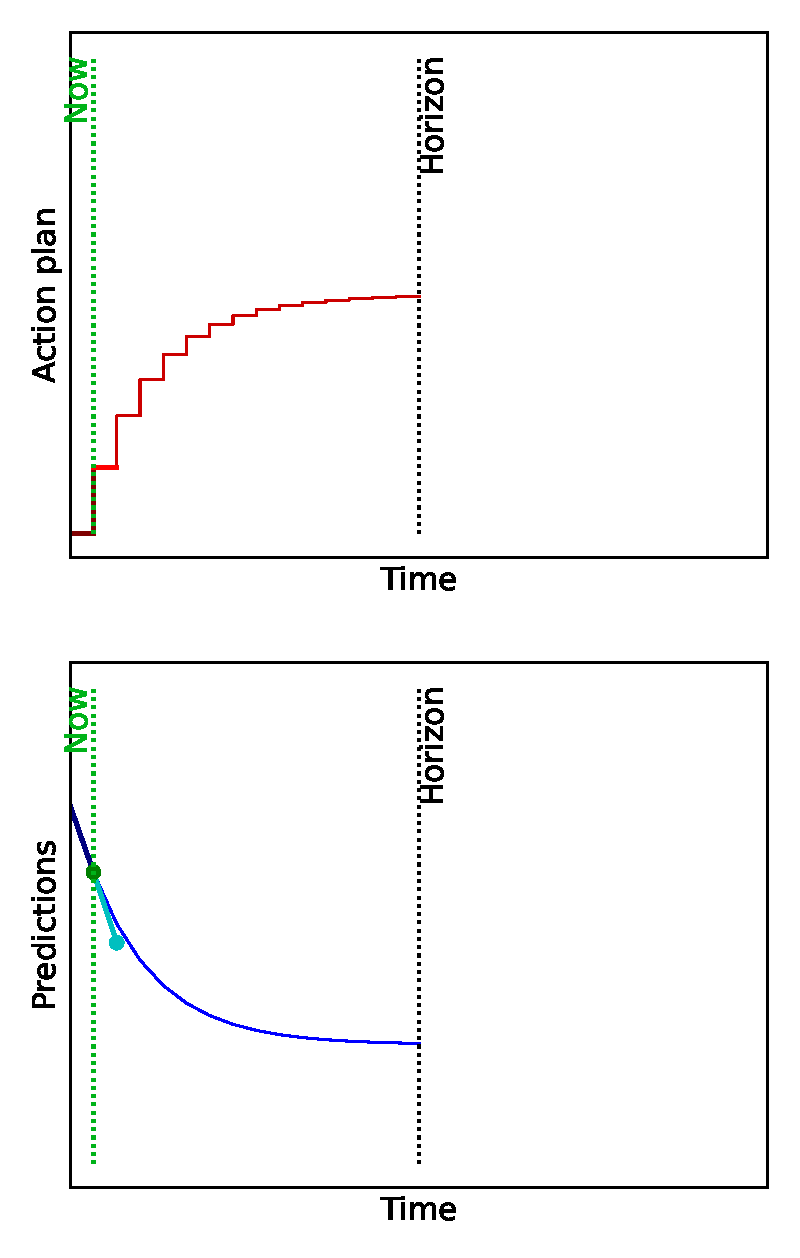
\includegraphics[width=\FS\textwidth,clip]{Codes/MPC/MPC1.eps}
        }%
              \only<3>
        {%
         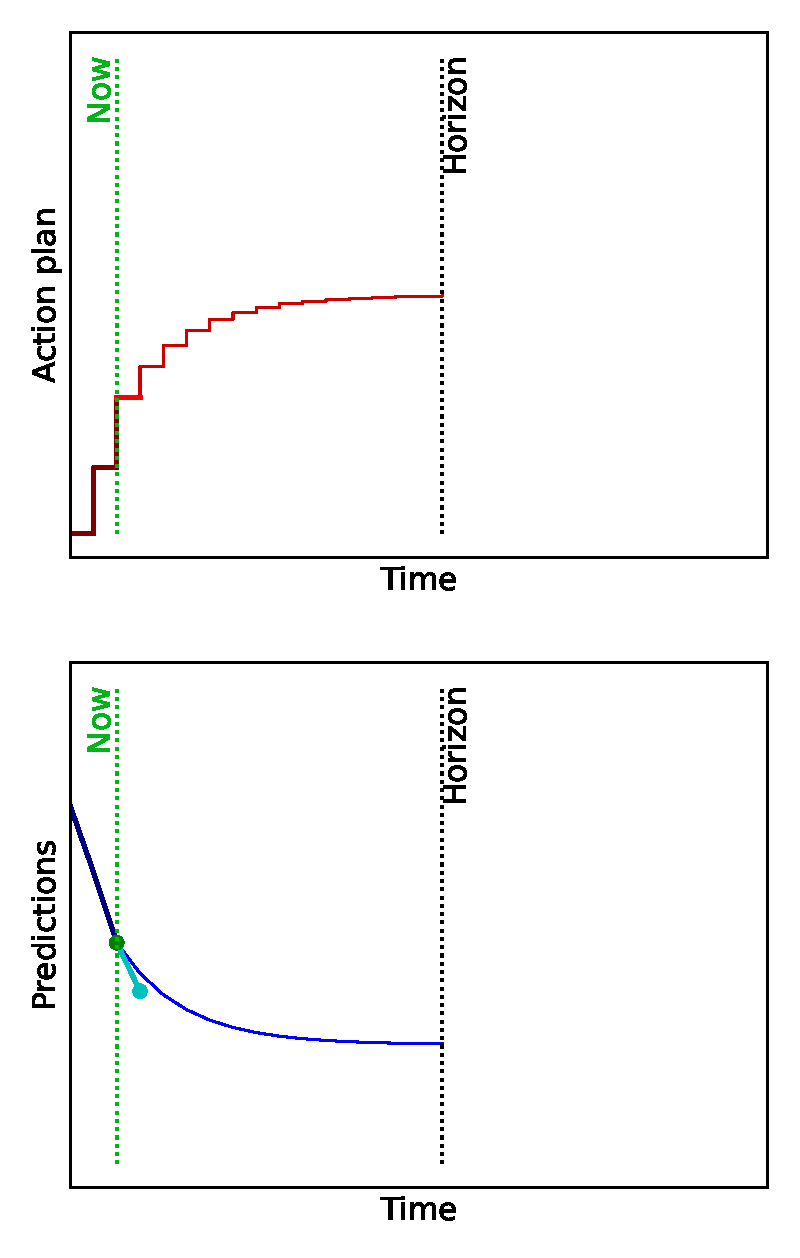
\includegraphics[width=\FS\textwidth,clip]{Codes/MPC/MPC2.eps}
        }%
              \only<4>
        {%
         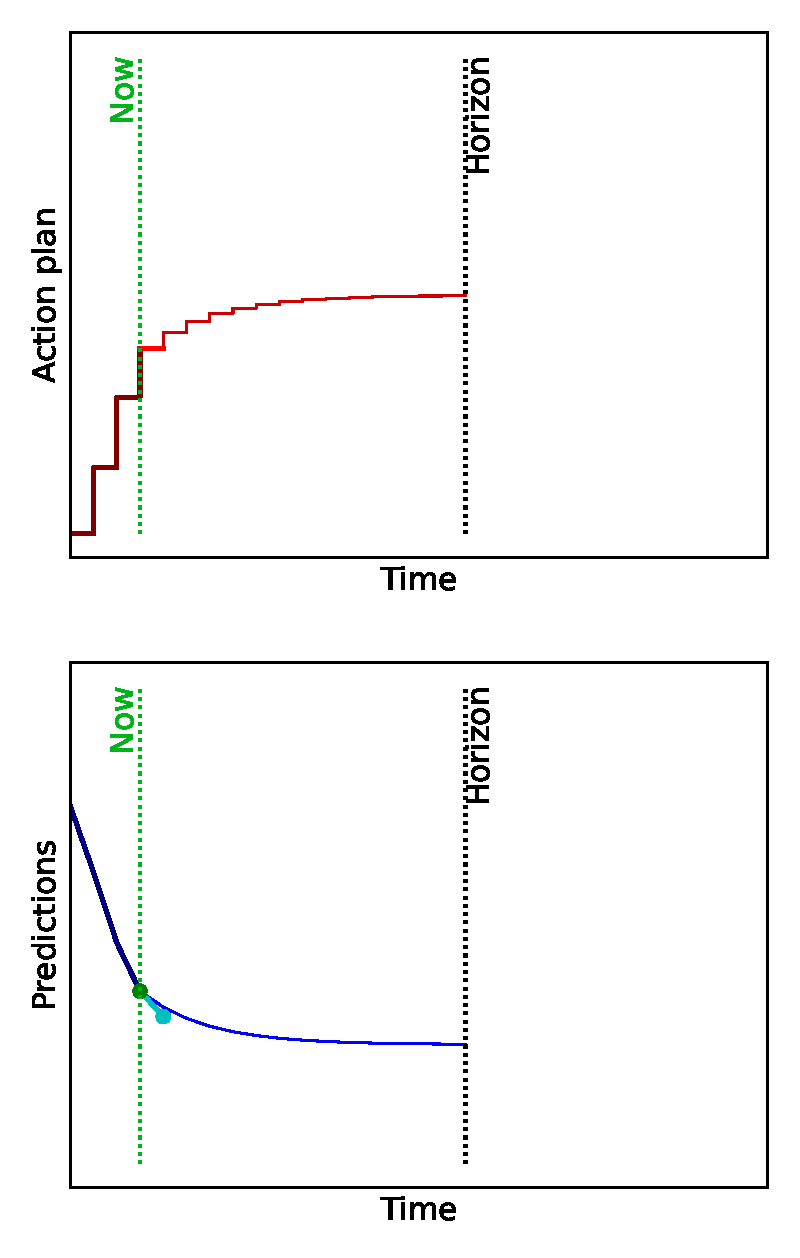
\includegraphics[width=\FS\textwidth,clip]{Codes/MPC/MPC3.eps}
        }%
              \only<5>
        {%
         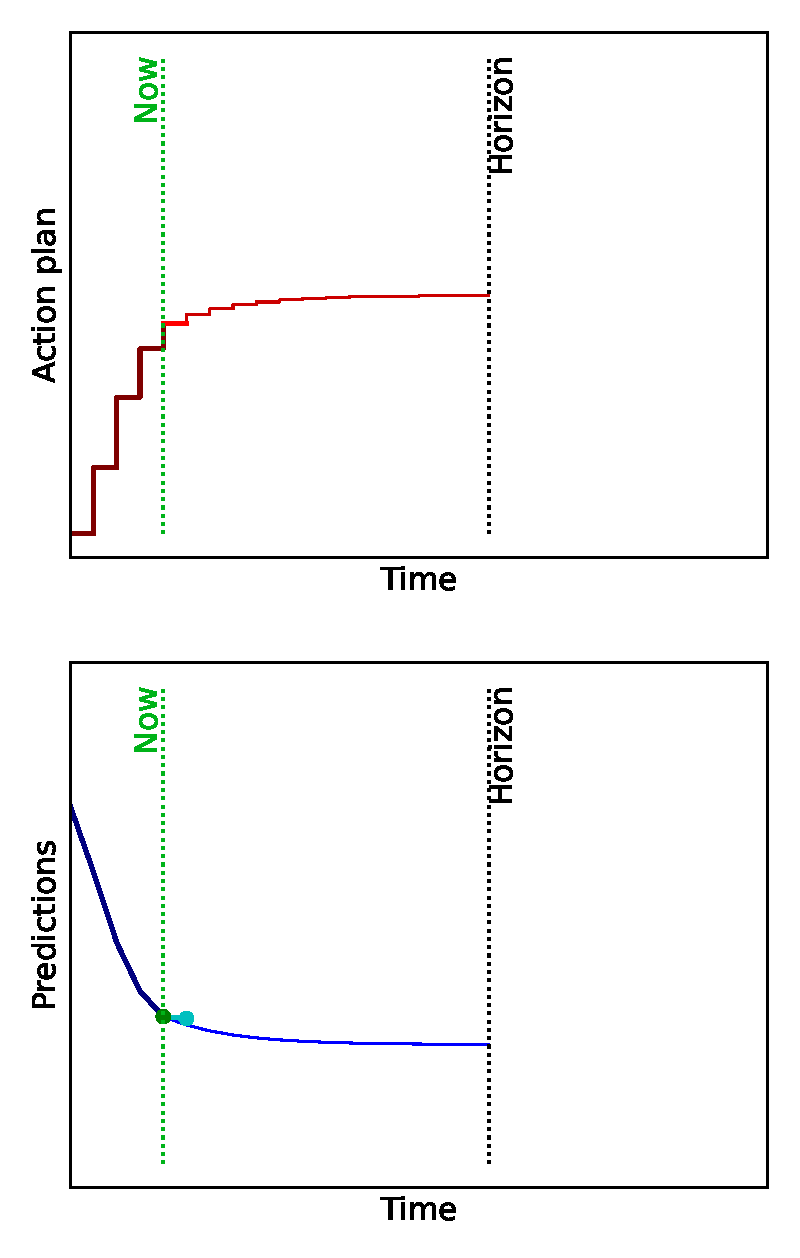
\includegraphics[width=\FS\textwidth,clip]{Codes/MPC/MPC4.eps}
        }%
              \only<6>
        {%
         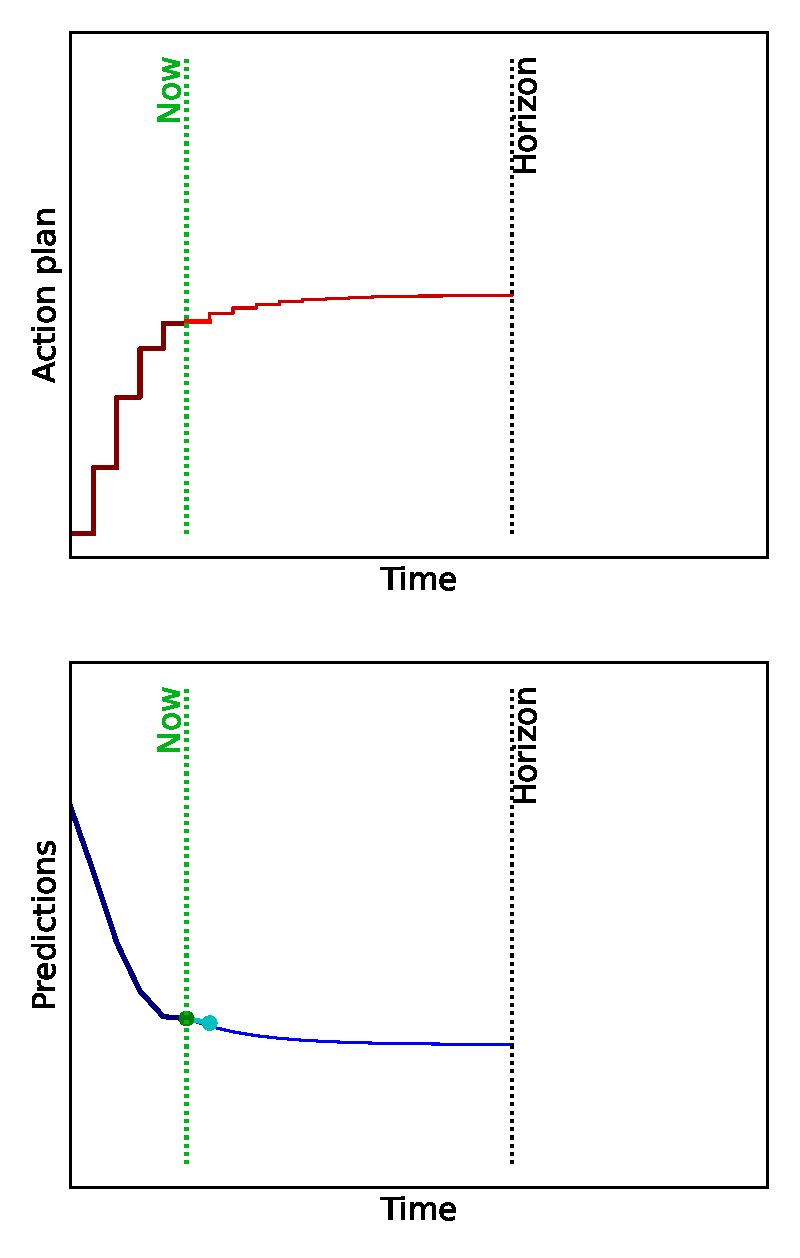
\includegraphics[width=\FS\textwidth,clip]{Codes/MPC/MPC5.eps}
        }%
              \only<7>
        {%
         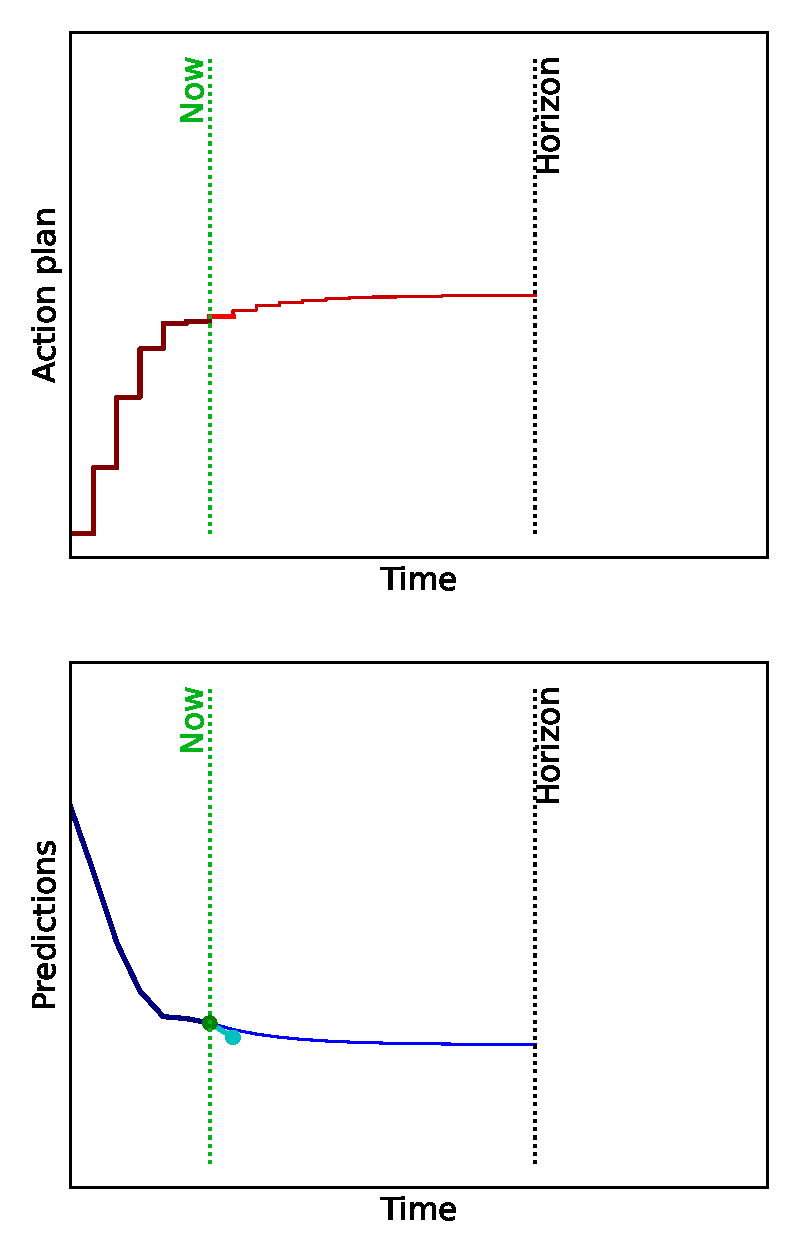
\includegraphics[width=\FS\textwidth,clip]{Codes/MPC/MPC6.eps}
        }%
              \only<8->
        {%
         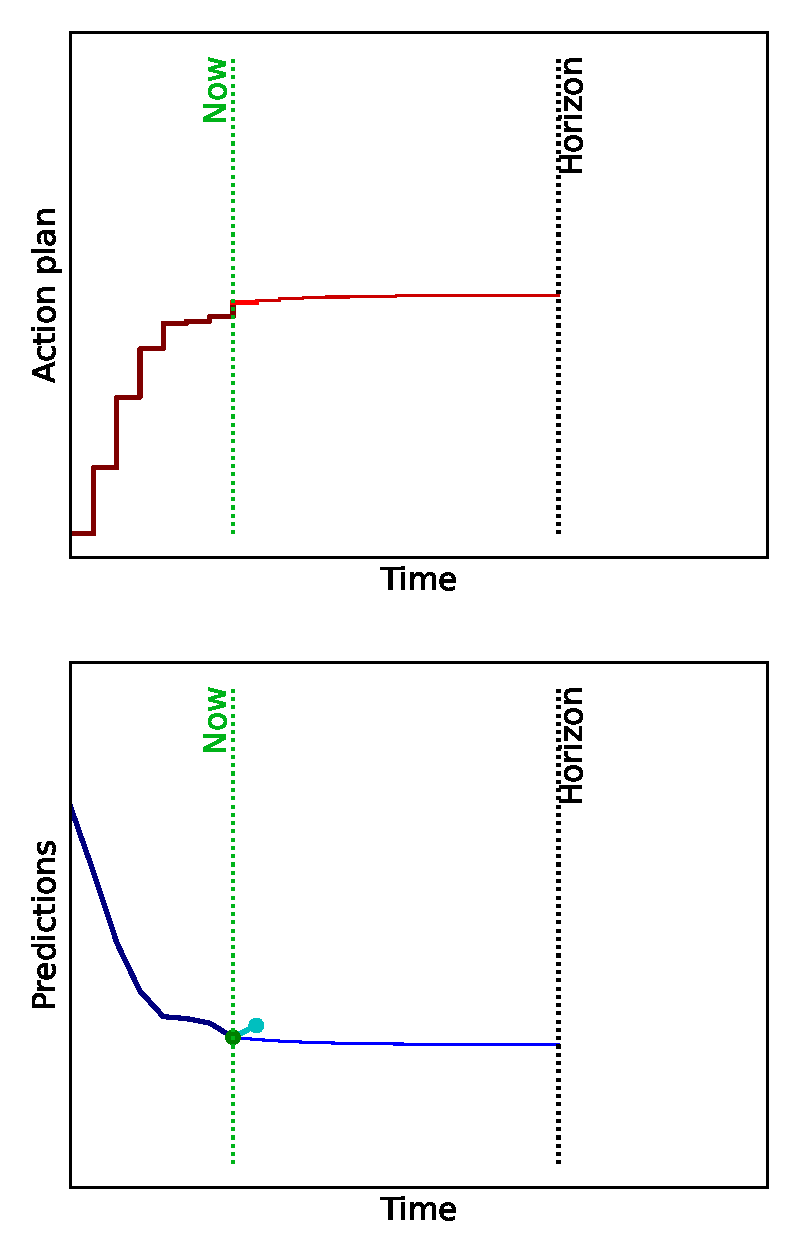
\includegraphics[width=\FS\textwidth,clip]{Codes/MPC/MPC7.eps}
        }%
        \end{figure}
  \end{overlayarea}
        


\column{0.6\textwidth}
\begin{block}{}
\textbf{Repeated Planning Strategy}
\vspace{-.1cm}
\begin{enumerate}
\scriptsize
\item\label{Info} Get up-to-date information
\item Optimize an \textcolor{myRed}{action plan} over a horizon
\begin{itemize}
\scriptsize
\item Use \textcolor{myBlue2}{predictions} to max utility \& respect constraints
\item Based on a model (AI or not)
\item Anchor at \textcolor{myGreen2}{current information (now)}
\end{itemize}
\item Implement first action of the plan
\item Back to \ref{Info}.%
\end{enumerate}
\end{block}
\visible<9->{
\textbf{Remarks}
\begin{itemize}
\scriptsize
\item Repeated Planning defines a decision policy
\begin{itemize}
\scriptsize
\item Mapping from information (1) to action (3)
\end{itemize}
\item Optimal plan $\Rightarrow$ optimal policy? 
\begin{itemize}
\tiny
\item It can if predictions are perfect
\item Imperfect model: complex relationship optimal plan / optimal policy (recently understood, more in a bit)
\end{itemize}
\item Terminology: MPC, Receding-Horizon Optimization, Planning, etc.
\end{itemize}
}
\end{columns}

\end{frame}


\begin{frame}{\normalsize Policies from Stochastic Planning}
\footnotesize

\begin{columns}
\column{0.4\textwidth}

  \begin{overlayarea}{\textwidth}{0.9\textheight}
    \begin{figure}
    \newcommand{\FS}{1}
      \centering
      \only<1>
        {%
          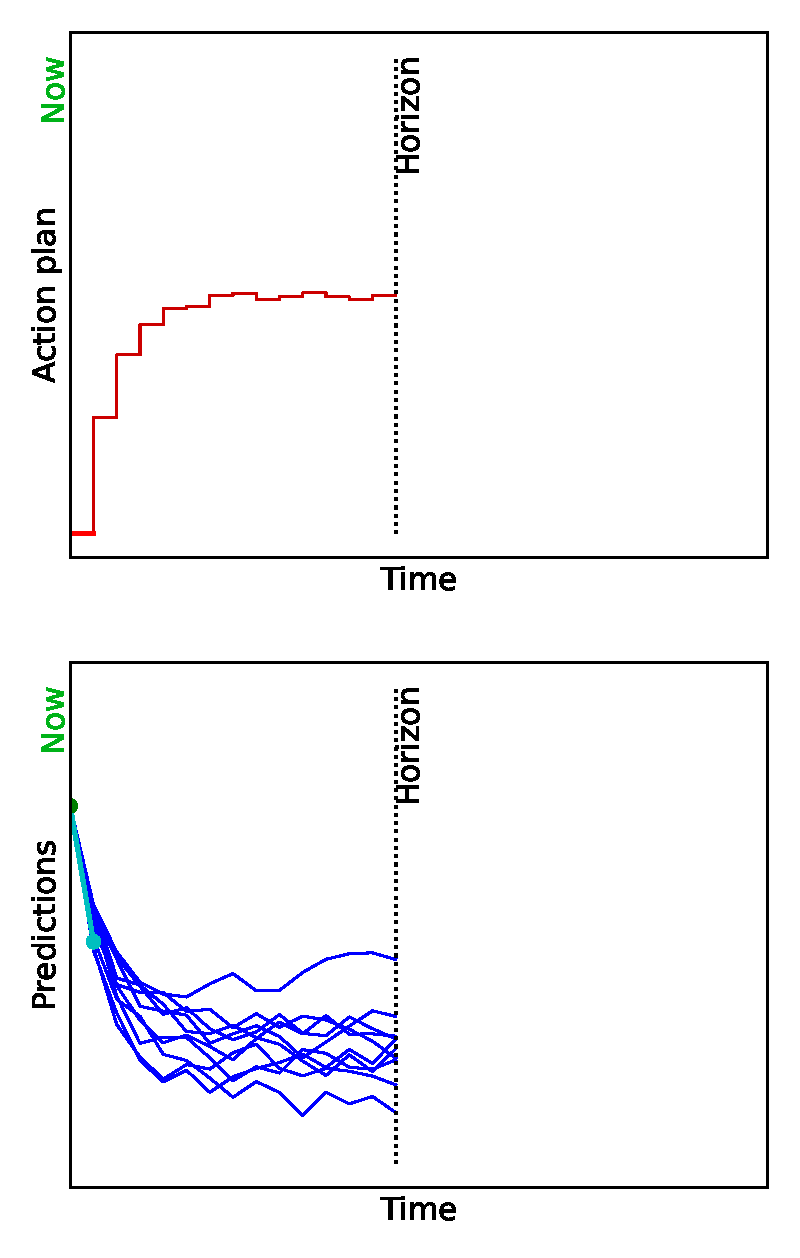
\includegraphics[width=\FS\textwidth,clip]{Codes/MPC/MPCMC0.eps}
        }%
              \only<2>
        {%
          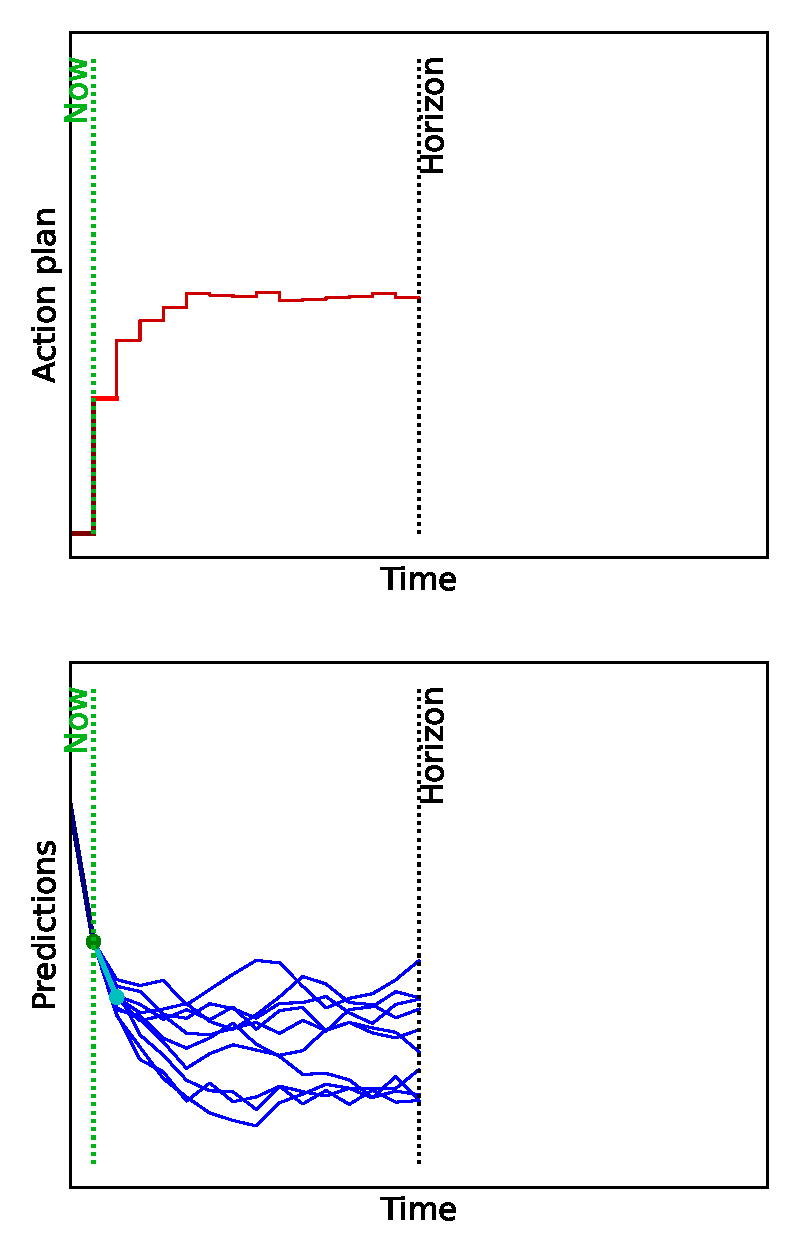
\includegraphics[width=\FS\textwidth,clip]{Codes/MPC/MPCMC1.eps}
        }%
              \only<3>
        {%
          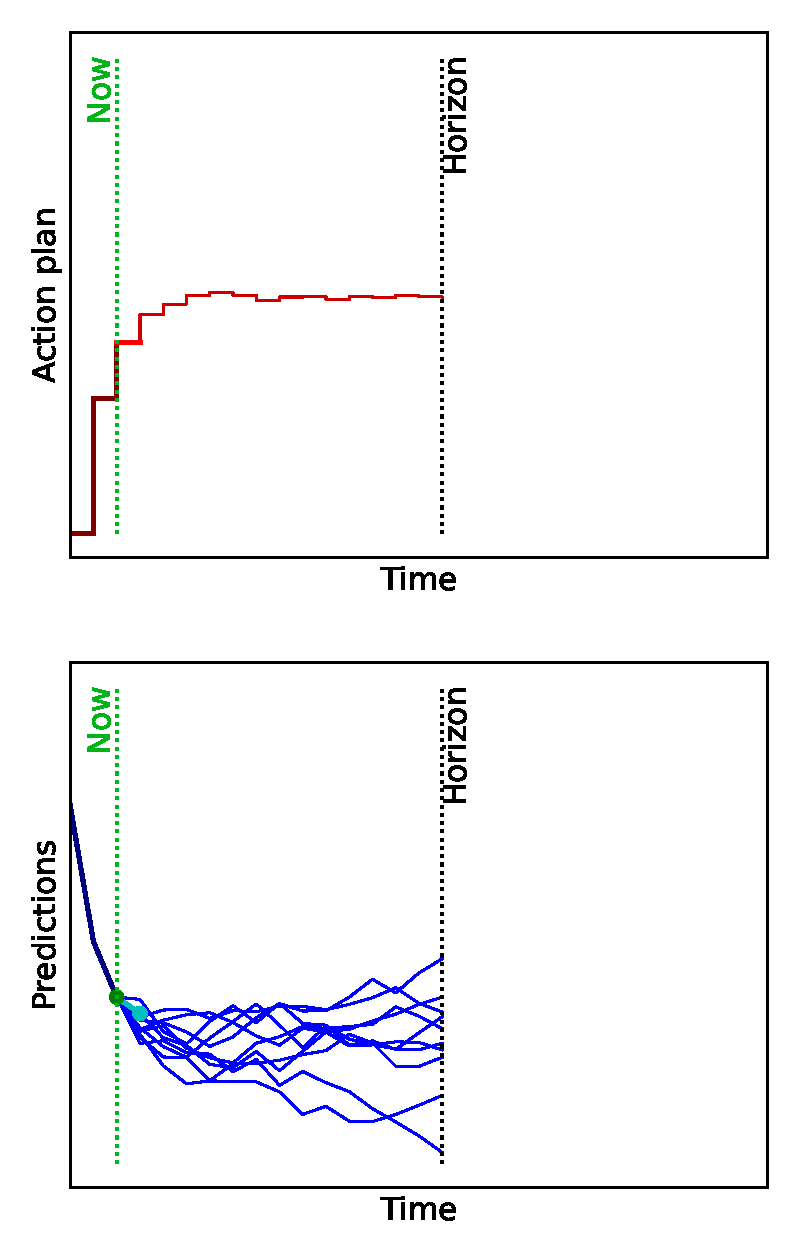
\includegraphics[width=\FS\textwidth,clip]{Codes/MPC/MPCMC2.eps}
        }%
              \only<4>
        {%
          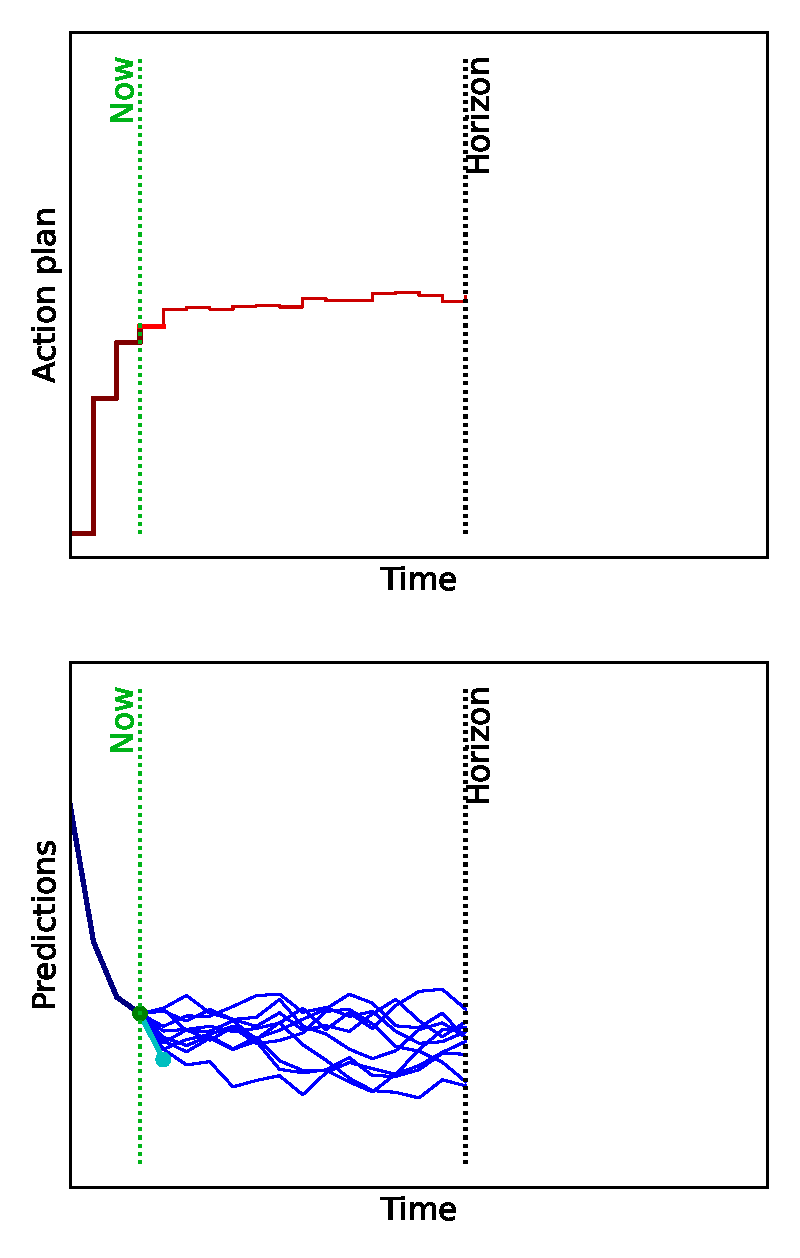
\includegraphics[width=\FS\textwidth,clip]{Codes/MPC/MPCMC3.eps}
        }%
              \only<5>
        {%
          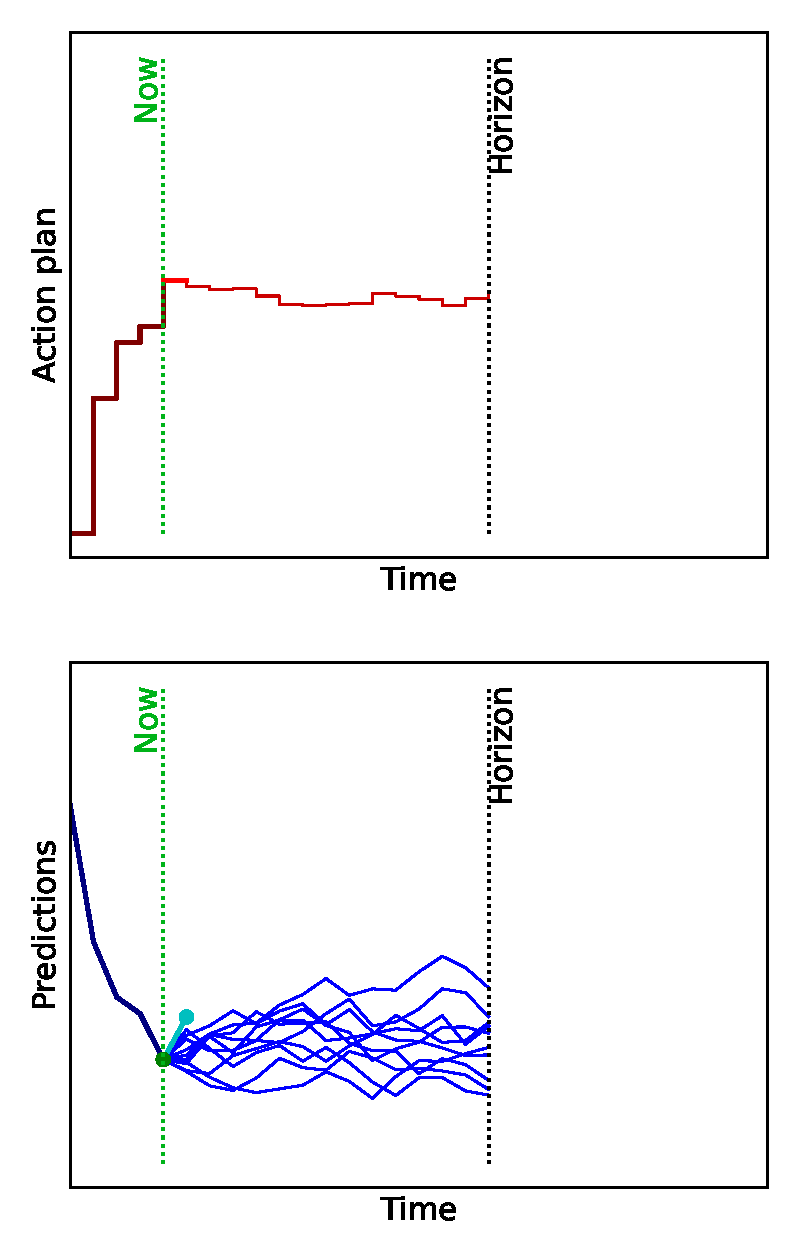
\includegraphics[width=\FS\textwidth,clip]{Codes/MPC/MPCMC4.eps}
        }%
              \only<6>
        {%
          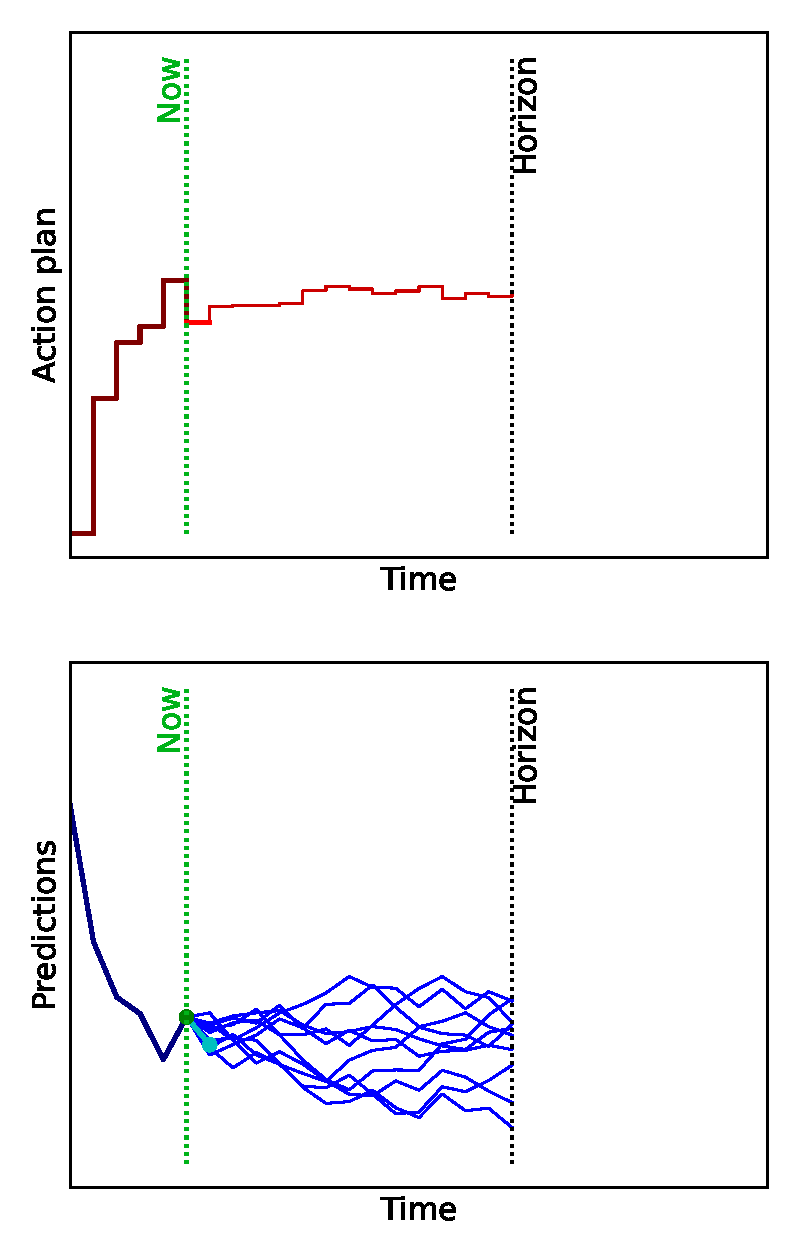
\includegraphics[width=\FS\textwidth,clip]{Codes/MPC/MPCMC5.eps}
        }%
              \only<7>
        {%
          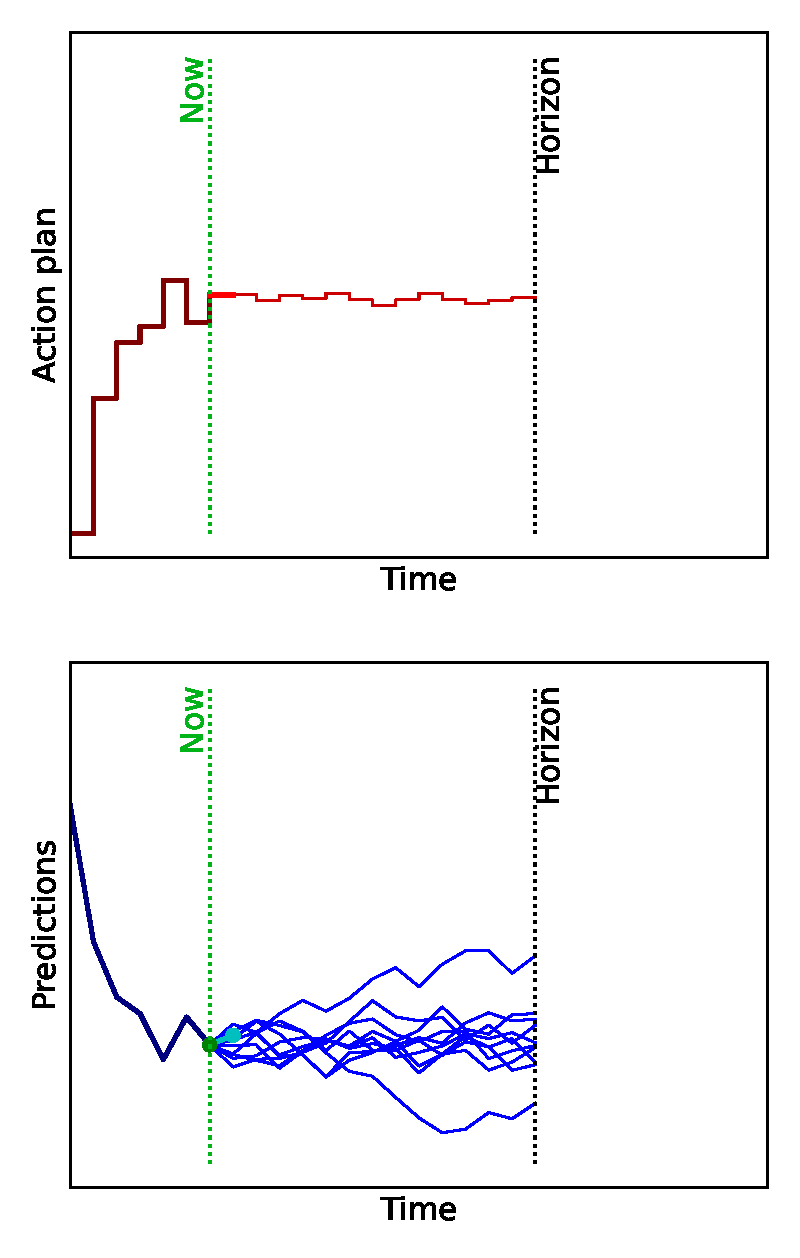
\includegraphics[width=\FS\textwidth,clip]{Codes/MPC/MPCMC6.eps}
        }%
              \only<8->
        {%
          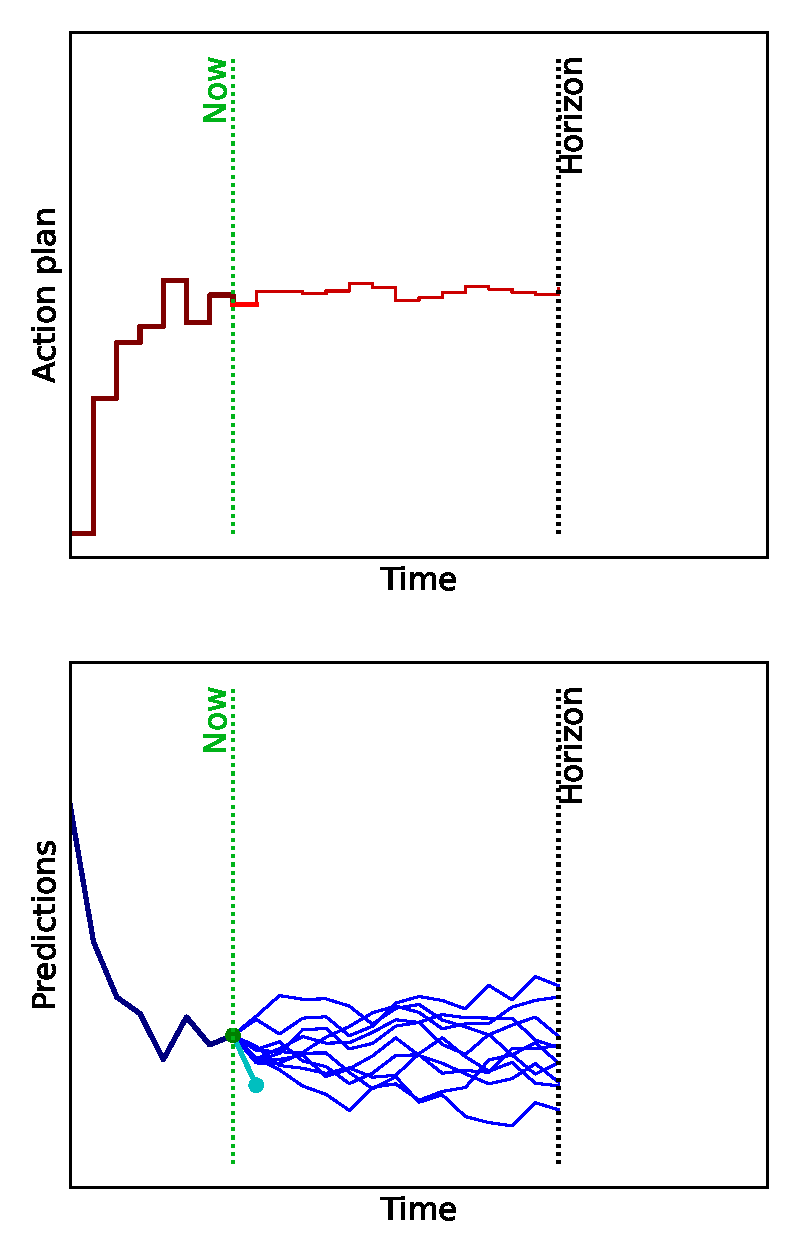
\includegraphics[width=\FS\textwidth,clip]{Codes/MPC/MPCMC7.eps}
        }%
    \end{figure}
  \end{overlayarea}  


%\begin{figure}
%\newcommand{\FS}{1}
%\includegraphics<1>[width=\FS\textwidth,clip]{Codes/MPC/MPCMC0.eps}
%\includegraphics<2>[width=\FS\textwidth,clip]{Codes/MPC/MPCMC1.eps}
%\includegraphics<3>[width=\FS\textwidth,clip]{Codes/MPC/MPCMC2.eps}
%\includegraphics<4>[width=\FS\textwidth,clip]{Codes/MPC/MPCMC3.eps}
%\includegraphics<5>[width=\FS\textwidth,clip]{Codes/MPC/MPCMC4.eps}
%\includegraphics<6>[width=\FS\textwidth,clip]{Codes/MPC/MPCMC5.eps}
%\includegraphics<7>[width=\FS\textwidth,clip]{Codes/MPC/MPCMC6.eps}
%\includegraphics<8->[width=\FS\textwidth,clip]{Codes/MPC/MPCMC7.eps}
%\end{figure}


\column{0.6\textwidth}
\begin{center}
\textbf{Same principle, but carry multiple predictions}
\end{center}
\visible<9->{
\textbf{Remarks}
\begin{itemize}
\scriptsize
\item Representative of real problem uncertainty: e.g. Monte Carlo sampling of probabilistic AI model
\item \visible<10->{Can select scenarios that are most relevant for decisions (not simple but doable)}
\visible<11->{
\item Setup
\begin{itemize}
\scriptsize
\item Max out utility: e.g. according to ``mean over predictions" (expected utility)
\item Constraints: all predictions must respect the constraints / probability of violation is at acceptable level
\end{itemize}}
\item \visible<12->{Planning still ignores that the action plan will be revised $\rightarrow$ conservative!}
\item \visible<13->{More advance model: scenario trees}
\end{itemize}}
\end{columns}


\end{frame}

\begin{frame}{\normalsize Policies from Scenario Trees}
\footnotesize

\begin{columns}
\column{0.5\textwidth}


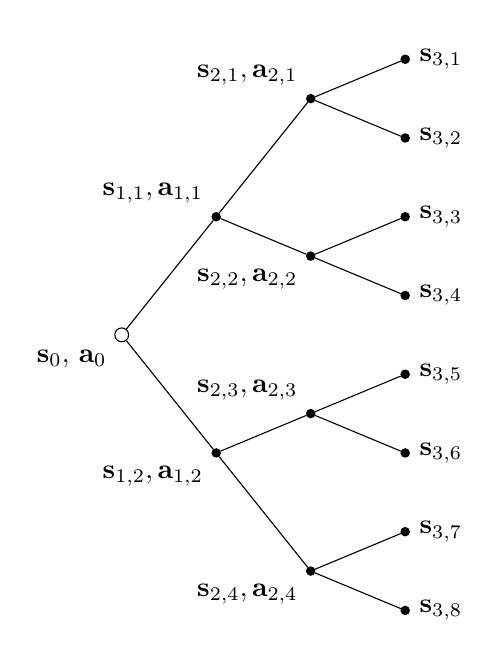
\begin{tikzpicture}
%Initial conditions
\draw (0,0)  node[draw,circle,fill=white,minimum size=5pt, inner sep=0pt, label = below left:{$\vect s_0,\,\vect a_0$}, label = {[xshift=-1cm, yshift=0.0cm]:{}}](sa) {};
%First branching
\draw (1.2,1.5)  node[draw,circle,fill=black,minimum size=3pt, inner sep=0pt, label=above left:{$\vect s_{1,1},\vect a_{1,1}$}, label = {[xshift=0.5cm, yshift=0.1cm]:{}}] (s11)  {};
\draw (1.2,-1.5) node[draw,circle,fill=black,minimum size=3pt, inner sep=0pt, label=below left:{$\vect s_{1,2},\vect a_{1,2}$}, label = {[xshift=0.5cm, yshift=0.1cm]:{}}] (s12)  {};
%Second branching
\visible<2->{\draw (2.4,3)  node[draw,circle,fill=black,minimum size=3pt, inner sep=0pt, label=above left:{$\vect s_{2,1},\vect a_{2,1}$}, label = {[xshift=0.5cm, yshift=0.1cm]:{}}] (s21)  {};}
\visible<2->{\draw (2.4,1)  node[draw,circle,fill=black,minimum size=3pt, inner sep=0pt, label=below left:{$\vect s_{2,2},\vect a_{2,2}$}, label = {[xshift=0.5cm, yshift=0.1cm]:{}}] (s22)  {};}
\visible<2->{\draw (2.4,-1)  node[draw,circle,fill=black,minimum size=3pt, inner sep=0pt, label=above left:{$\vect s_{2,3},\vect a_{2,3}$}, label = {[xshift=0.5cm, yshift=0.1cm]:{}}] (s23)  {};}
\visible<2->{\draw (2.4,-3) node[draw,circle,fill=black,minimum size=3pt, inner sep=0pt, label=below left:{$\vect s_{2,4},\vect a_{2,4}$}, label = {[xshift=0.5cm, yshift=0.1cm]:{}}] (s24)  {};}
%Third branching
\visible<3->{\draw (3.6,3.5)  node[draw,circle,fill=black,minimum size=3pt, inner sep=0pt, label=right:{$\vect s_{3,1}$}, label = {[xshift=0.5cm, yshift=0.1cm]:{}}] (s31)  {}; }%,\vect u_{3,1}
\visible<3->{\draw (3.6,2.5)  node[draw,circle,fill=black,minimum size=3pt, inner sep=0pt, label=right:{$\vect s_{3,2}$}, label = {[xshift=0.5cm, yshift=0.1cm]:{}}] (s32)  {}; }%,\vect u_{3,2}
\visible<3->{\draw (3.6,1.5)  node[draw,circle,fill=black,minimum size=3pt, inner sep=0pt, label=right:{$\vect s_{3,3}$}, label = {[xshift=0.5cm, yshift=0.1cm]:{}}] (s33)  {}; }%,\vect u_{3,3}
\visible<3->{\draw (3.6,0.5) node[draw,circle,fill=black,minimum size=3pt, inner sep=0pt, label=right:{$\vect s_{3,4}$}, label = {[xshift=0.5cm, yshift=0.1cm]:{}}] (s34)  {}; }%,\vect u_{3,4}
\visible<3->{\draw (3.6,-0.5)  node[draw,circle,fill=black,minimum size=3pt, inner sep=0pt, label=right:{$\vect s_{3,5}$}, label = {[xshift=0.5cm, yshift=0.1cm]:{}}] (s35)  {};} %,\vect u_{3,5}
\visible<3->{\draw (3.6,-1.5)  node[draw,circle,fill=black,minimum size=3pt, inner sep=0pt, label=right:{$\vect s_{3,6}$}, label = {[xshift=0.5cm, yshift=0.1cm]:{}}] (s36)  {}; }%,\vect u_{3,6}
\visible<3->{\draw (3.6,-2.5)  node[draw,circle,fill=black,minimum size=3pt, inner sep=0pt, label=right:{$\vect s_{3,7}$}, label = {[xshift=0.5cm, yshift=0.1cm]:{}}] (s37)  {}; }%,\vect u_{3,7}
\visible<3->{\draw (3.6,-3.5) node[draw,circle,fill=black,minimum size=3pt, inner sep=0pt, label=right:{$\vect s_{3,8}$}, label = {[xshift=0.5cm, yshift=0.1cm]:{}}] (s38)  {}; }%,\vect u_{3,8}

\path
(sa) edge node[above, xshift=0.0cm, yshift=0.275cm]{} (s11)
(sa) edge node[below, xshift=0.0cm, yshift=-0.275cm]{} (s12);
 
%Second branching
 \visible<2->{\path (s11) edge node[above, xshift=0.0cm, yshift=0.275cm]{} (s21);}
 \visible<2->{\path (s11) edge node[above, xshift=0.0cm, yshift=0.275cm]{} (s22);}
 
 \visible<2->{\path (s12) edge node[above, xshift=0.0cm, yshift=0.275cm]{} (s23);}
 \visible<2->{\path (s12) edge node[above, xshift=0.0cm, yshift=0.275cm]{} (s24);}
 
 %Third branching
 \visible<3->{\path (s21) edge node[above, xshift=0.0cm, yshift=0.275cm]{} (s31);}
 \visible<3->{\path(s21) edge node[above, xshift=0.0cm, yshift=0.275cm]{} (s32);}
 
 \visible<3->{\path(s22) edge node[above, xshift=0.0cm, yshift=0.275cm]{} (s33);}
 \visible<3->{\path(s22) edge node[above, xshift=0.0cm, yshift=0.275cm]{} (s34);}
 
 \visible<3->{\path(s23) edge node[above, xshift=0.0cm, yshift=0.275cm]{} (s35);}
 \visible<3->{\path(s23) edge node[above, xshift=0.0cm, yshift=0.275cm]{} (s36);}
 
 \visible<3->{\path(s24) edge node[above, xshift=0.0cm, yshift=0.275cm]{} (s37);}
 \visible<3->{\path(s24) edge node[above, xshift=0.0cm, yshift=0.275cm]{} (s38);}
\end{tikzpicture}        


\column{0.5\textwidth}
\begin{center}
\textbf{Model different outcomes and associated decisions}
\end{center}
\visible<4->{
\textbf{Remarks}: 
\begin{itemize}
\scriptsize
\item Very coarse model of uncertainty: each ``branching" represents a small amount of possibilities
\item Exploding complexity over planning horizon, keep it short
\item See Mutli-Stage Stochastic Programming
\end{itemize}}

\end{columns}


\end{frame}





\section{Some Fundamentals of Decision Making Theory}


\begin{frame}{\normalsize Markov State}
\footnotesize

\textbf{Markov State:} often labelled $\vect s$
\begin{itemize}
\scriptsize
\item Is often a collection of numbers, i.e. $\vect s\in \mathbb R^n$, but it can be ``anything"
\item Evolves over time, e.g. label $\vect s_k$ with $k=0,\ldots,\infty$
\item Usually stochastic 
\end{itemize}
\visible<2->{
\textbf{Definition}: $\vect s_k$ provides a ``complete statistics" of the past sufficient to predict $\vect s_{k+1,\ldots,\infty}$.} 
\begin{center}
\visible<3->{More formally: $\mathrm{P}\left[\vect s_{k+i}\,|\, \vect\pi,\vect s_k\right] = \mathrm{P}\left[\vect s_{k+i}\,|\, \vect\pi,\vect s_k, \vect s_{k-1},\ldots, \vect s_0\right]$ for any $i>0$, $\vect \pi$}\\
\vspace{.25cm}
\visible<4->{
\textcolor{myBlue2}{I.e. state $\vect s_k$ collects all the information to predict the future (after $k$). \\ Past states $\vect s_{k-1,\ldots,0}$ do not add information}
}
\end{center}

  \begin{overlayarea}{\textwidth}{0.55\textheight}
    \begin{figure}
    \newcommand{\FS}{0.7}
      \centering
      \only<5>
        {%
          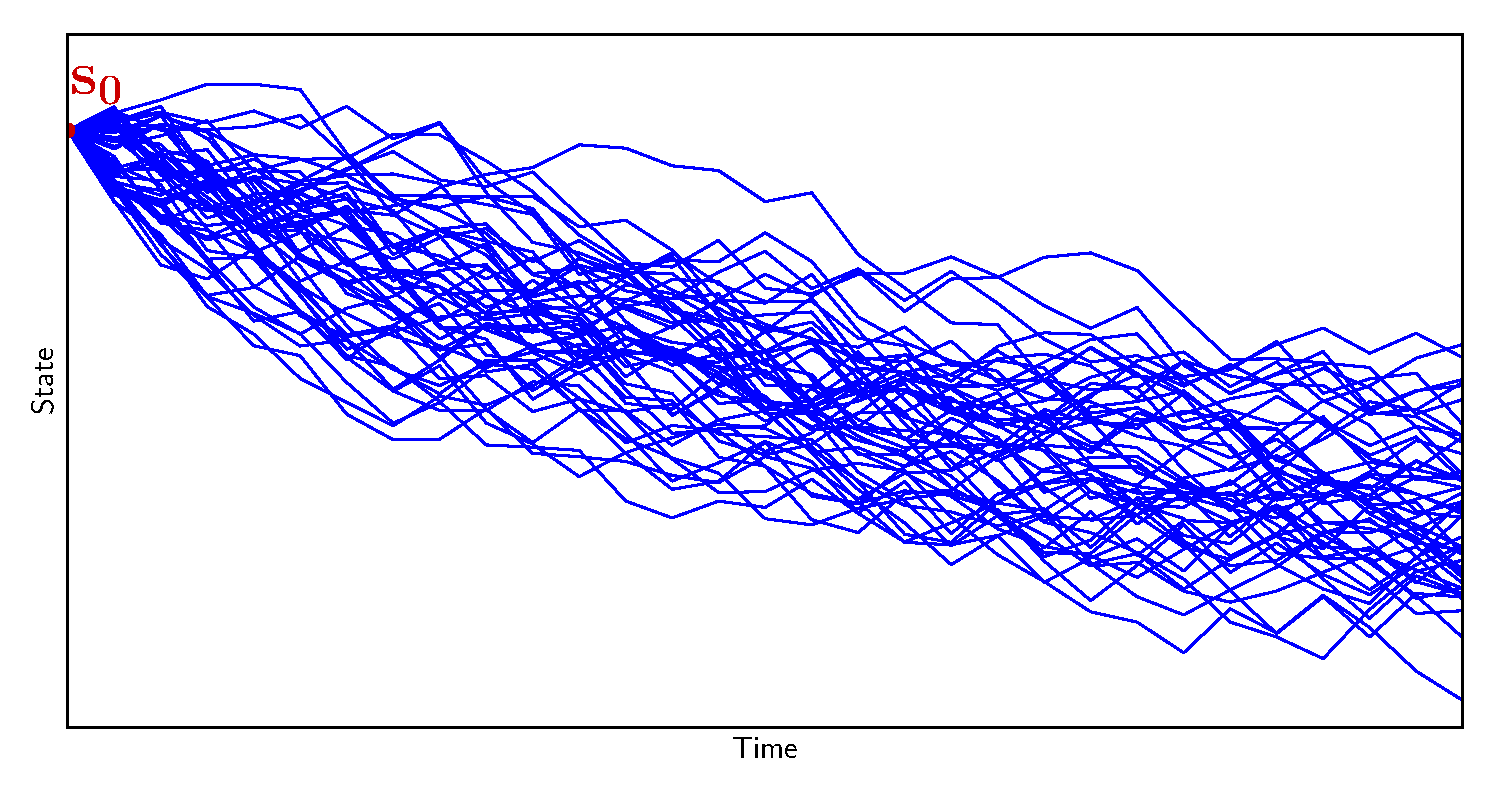
\includegraphics[width=\FS\textwidth,clip]{Codes/Basics/Markov0.eps}
        }%
      \only<6>
        {%
          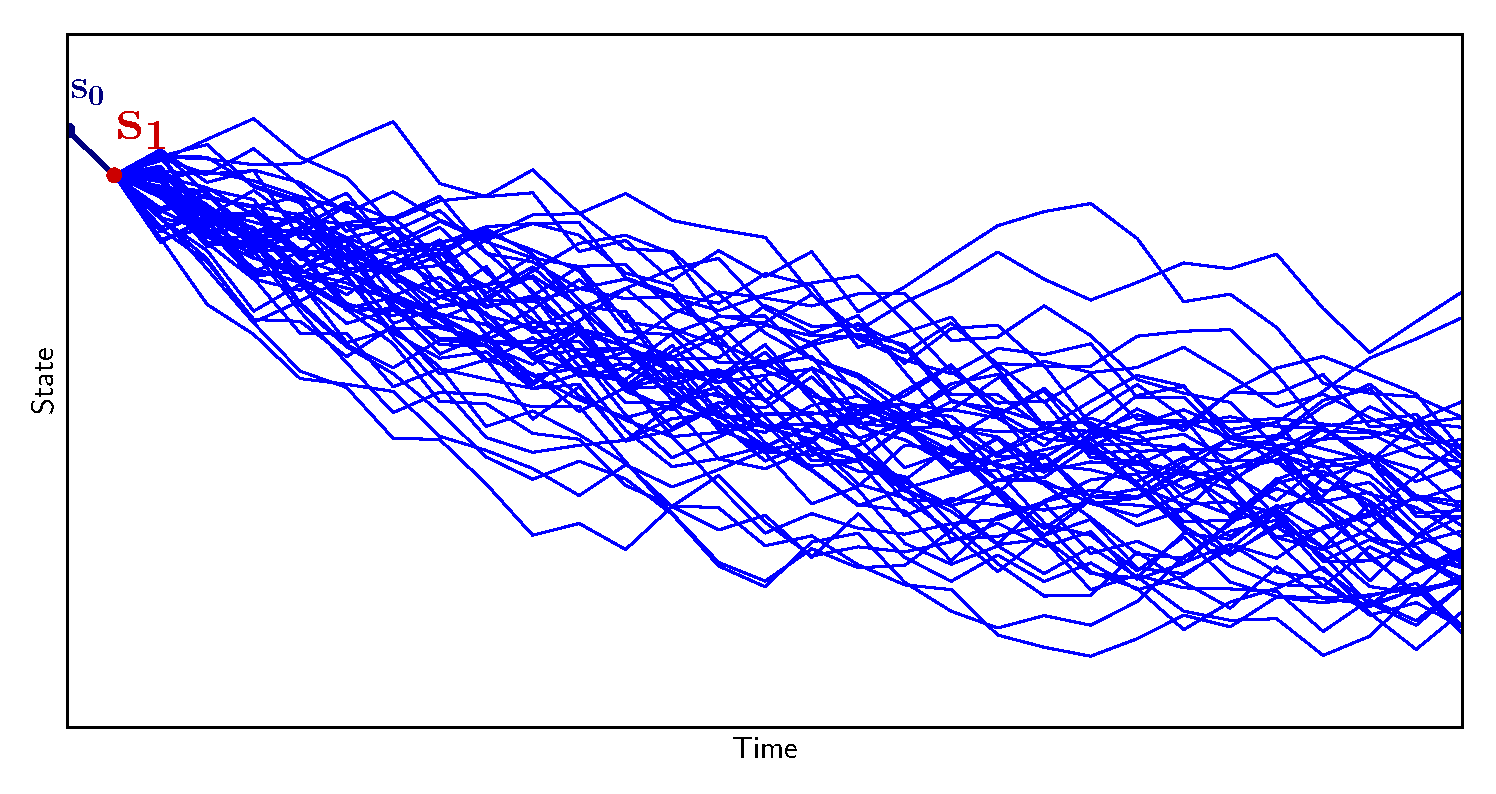
\includegraphics[width=\FS\textwidth,clip]{Codes/Basics/Markov1.eps}
        }%
              \only<7>
        {%
          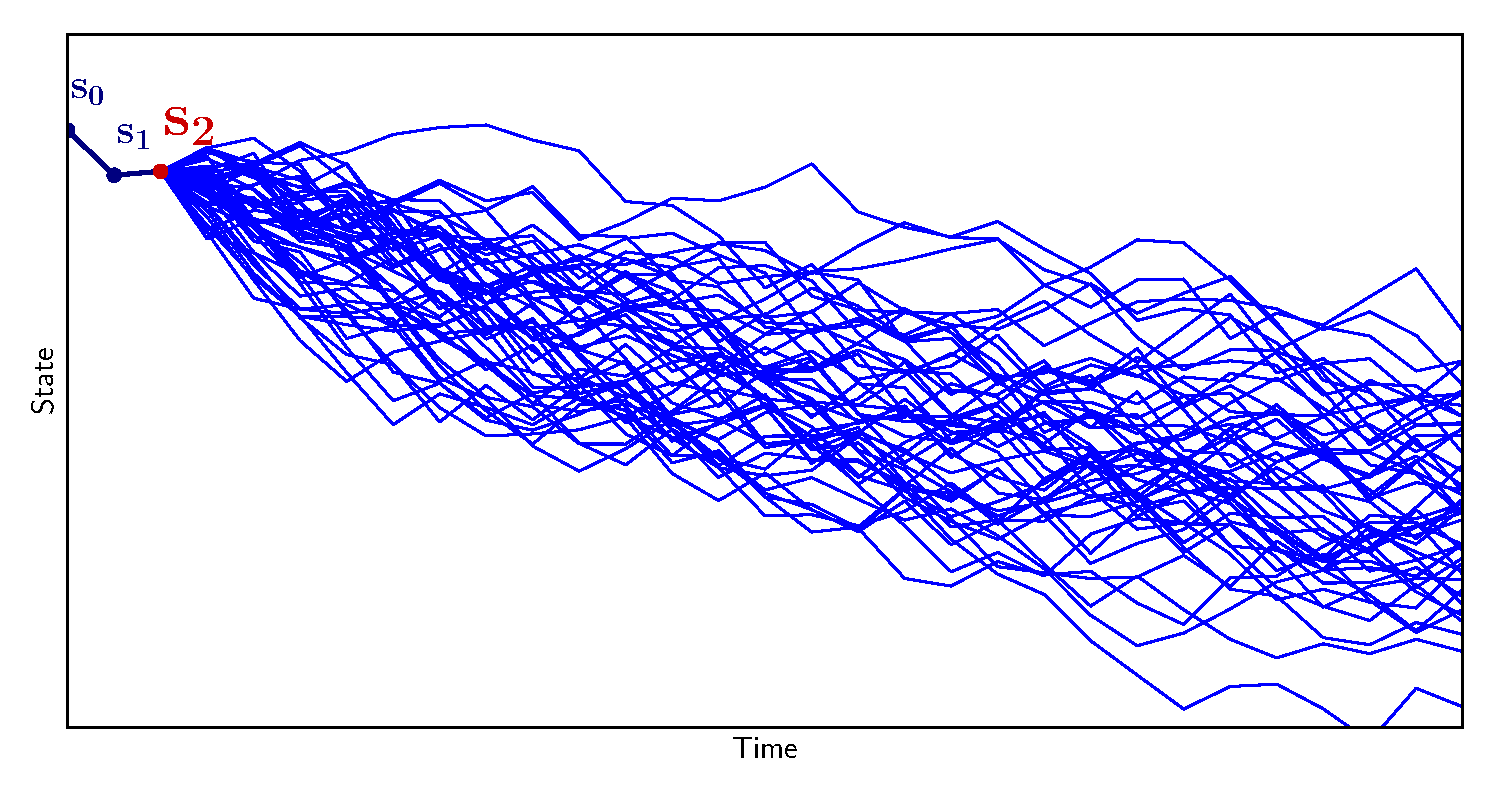
\includegraphics[width=\FS\textwidth,clip]{Codes/Basics/Markov2.eps}
        }%
              \only<8>
        {%
          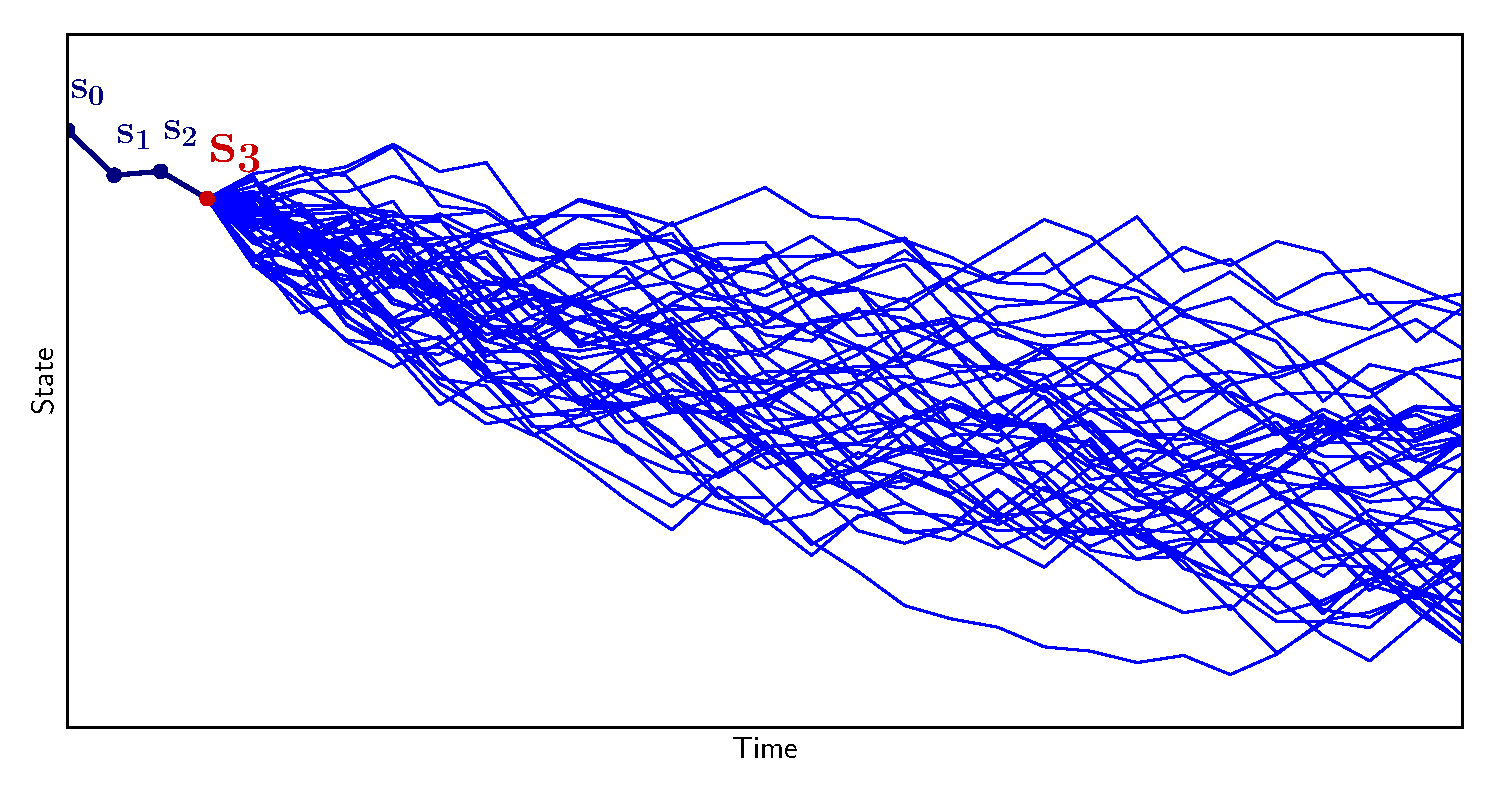
\includegraphics[width=\FS\textwidth,clip]{Codes/Basics/Markov3.eps}
        }%
              \only<9>
        {%
          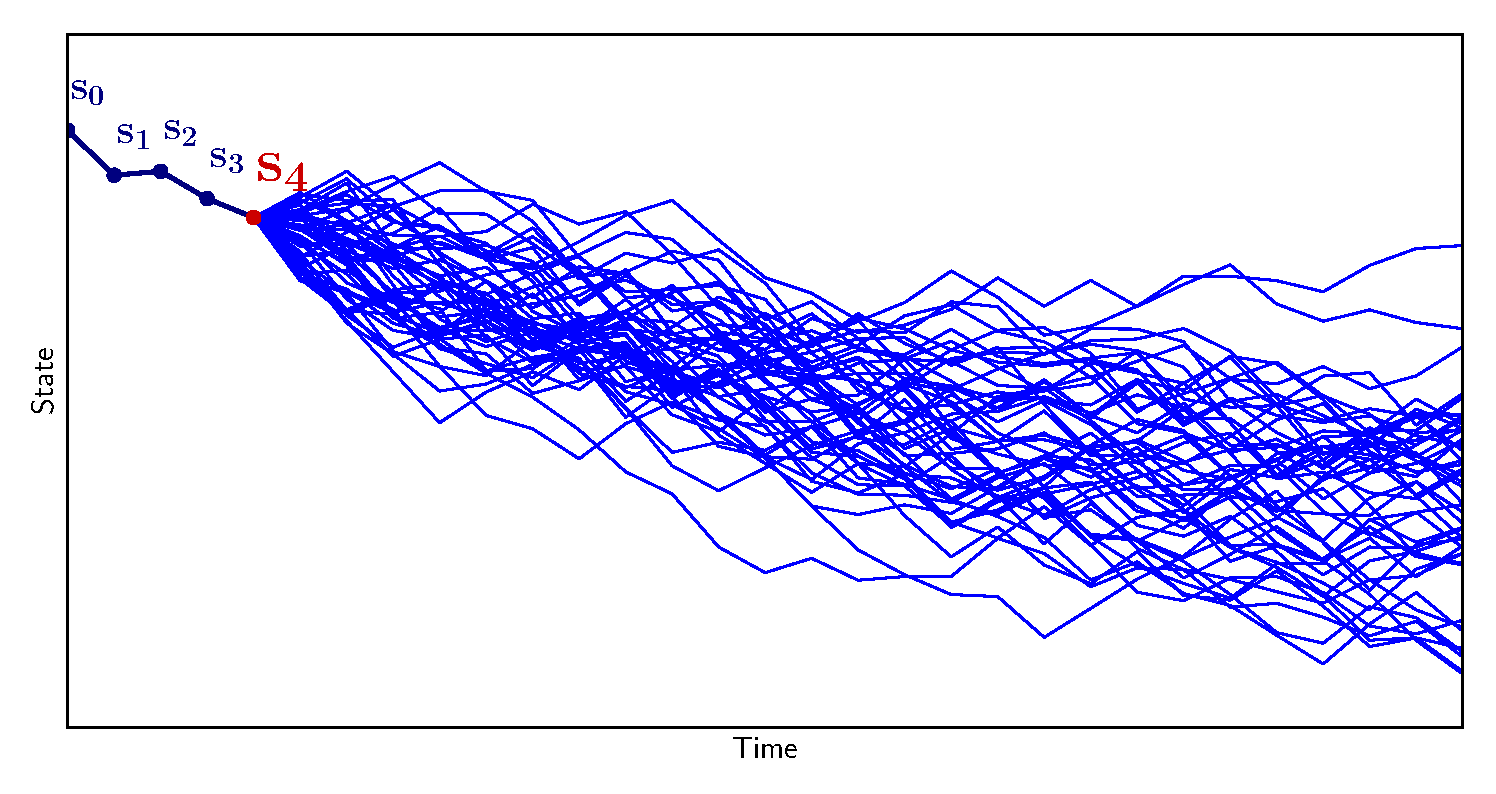
\includegraphics[width=\FS\textwidth,clip]{Codes/Basics/Markov4.eps}
        }%
              \only<10>
        {%
          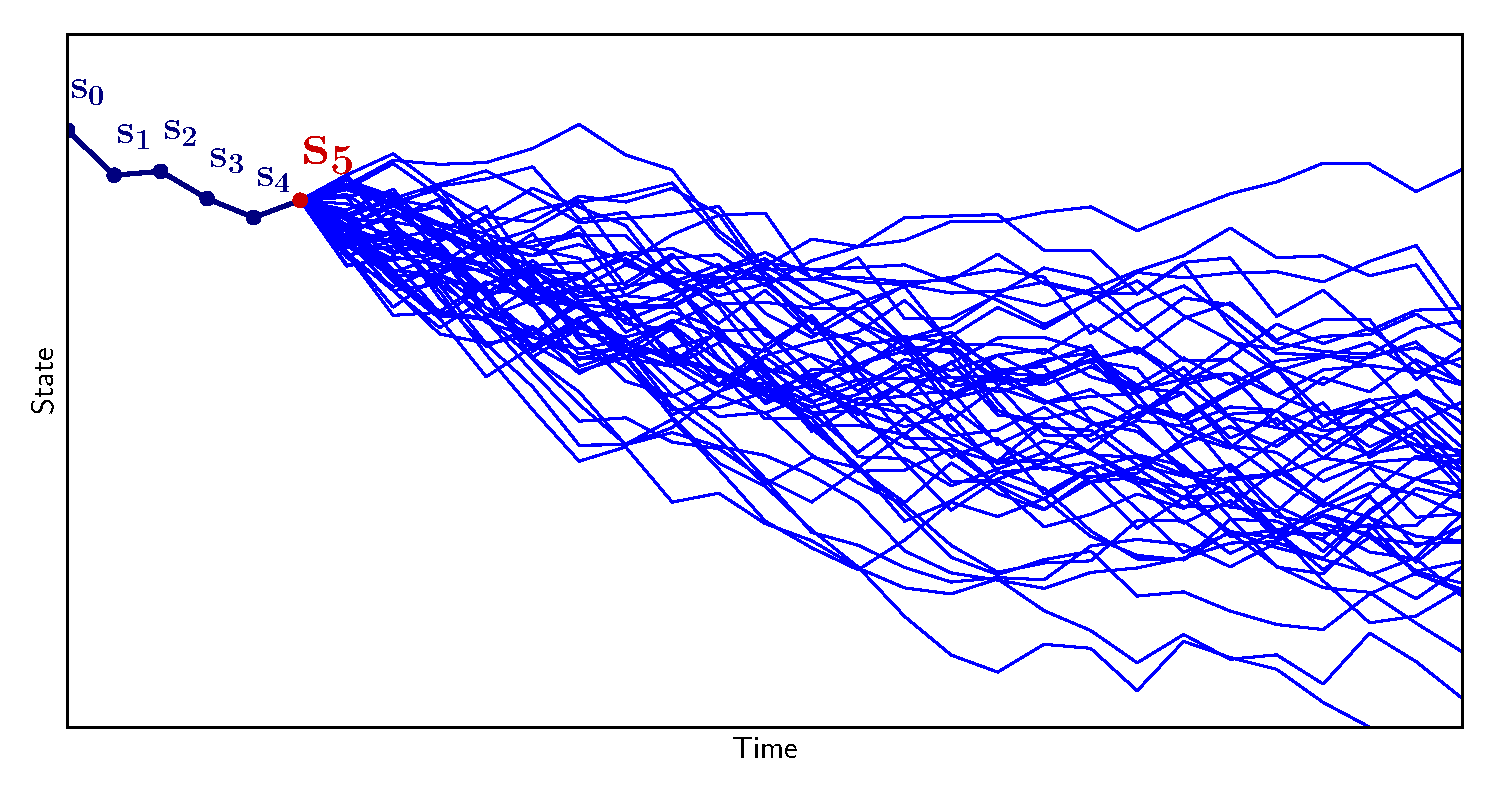
\includegraphics[width=\FS\textwidth,clip]{Codes/Basics/Markov5.eps}
        }%
              \only<11>
        {%
          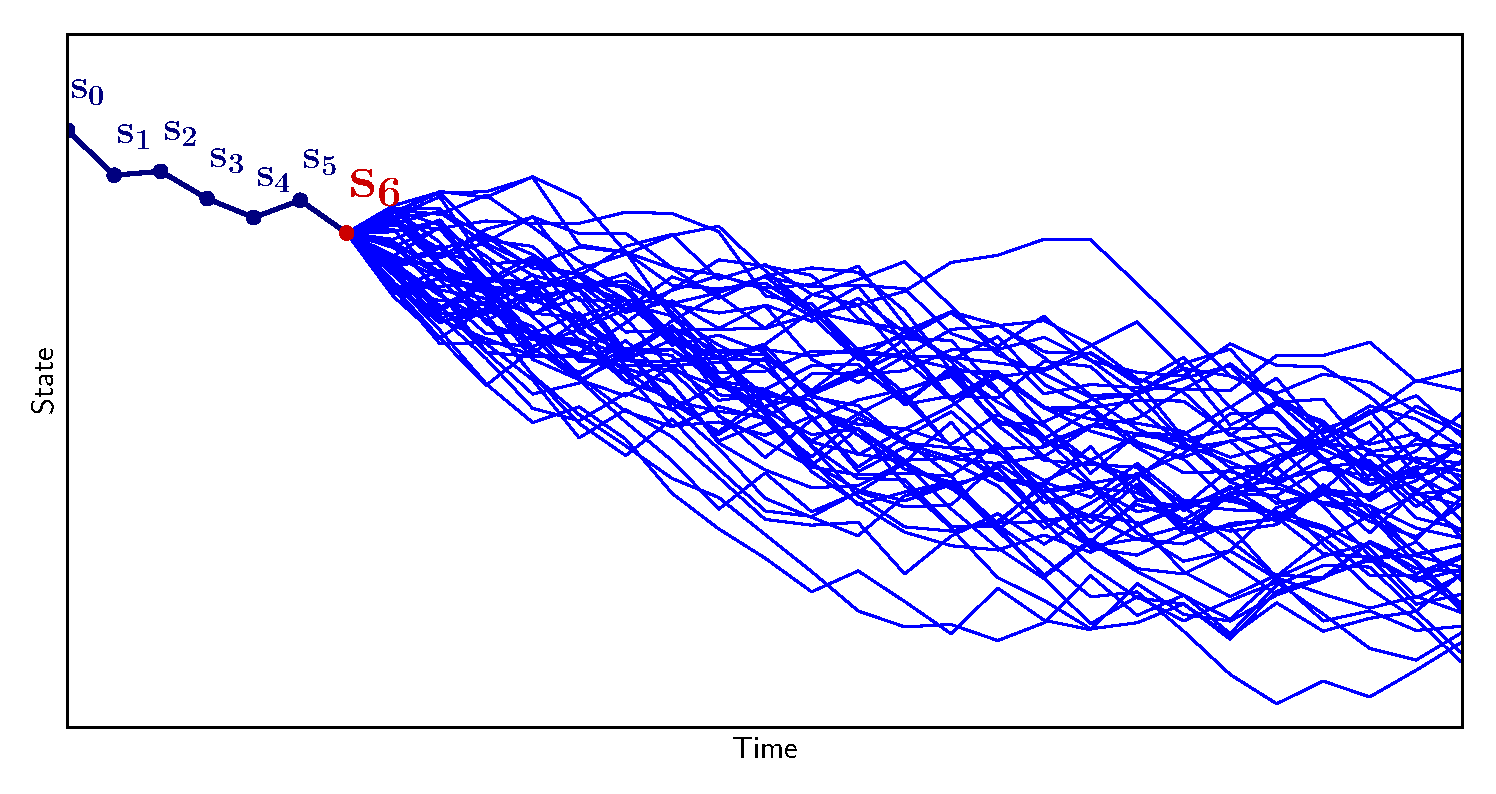
\includegraphics[width=\FS\textwidth,clip]{Codes/Basics/Markov6.eps}
        }%
              \only<12>
        {%
          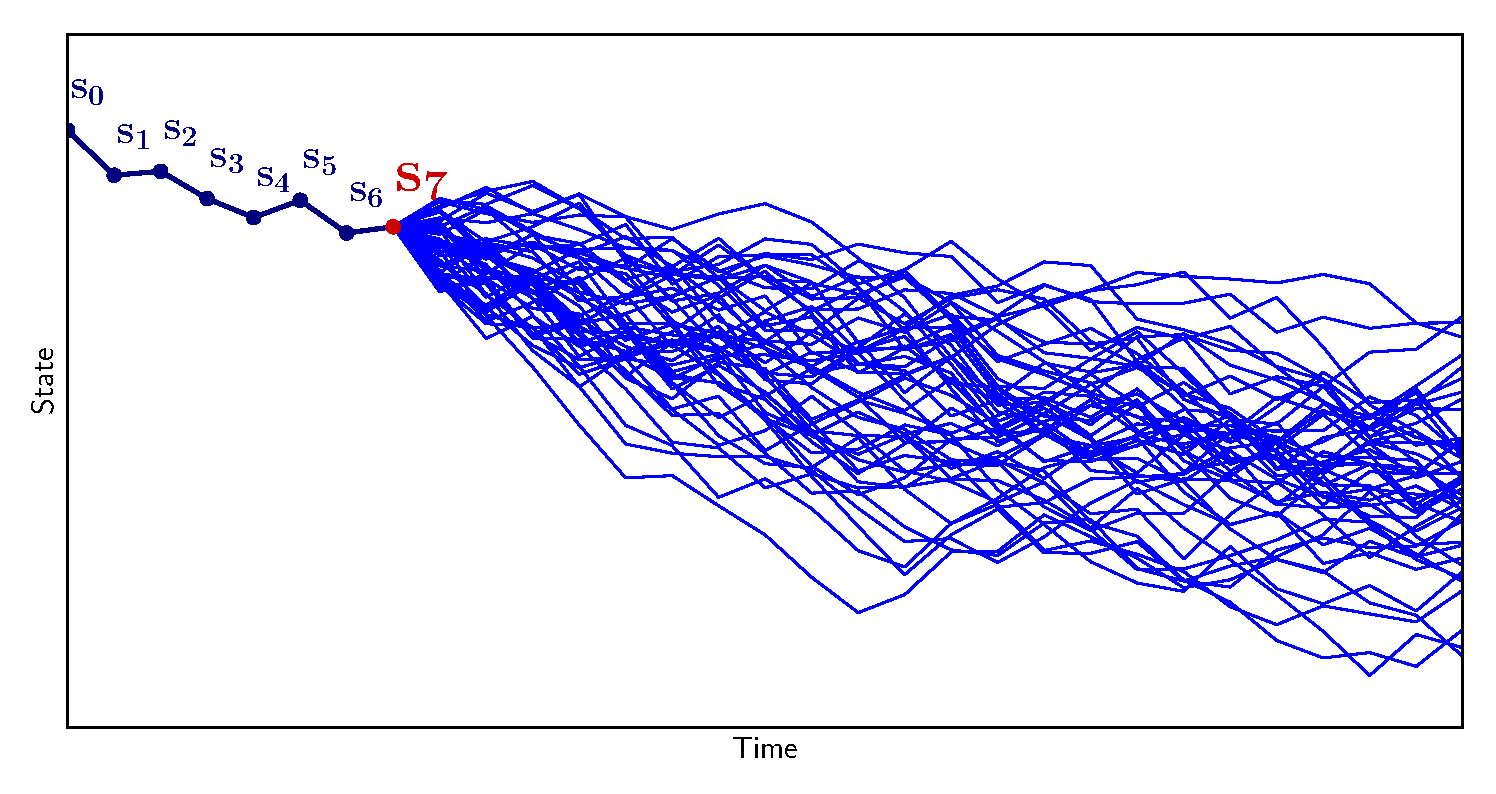
\includegraphics[width=\FS\textwidth,clip]{Codes/Basics/Markov7.eps}
        }%
              \only<13>
        {%
          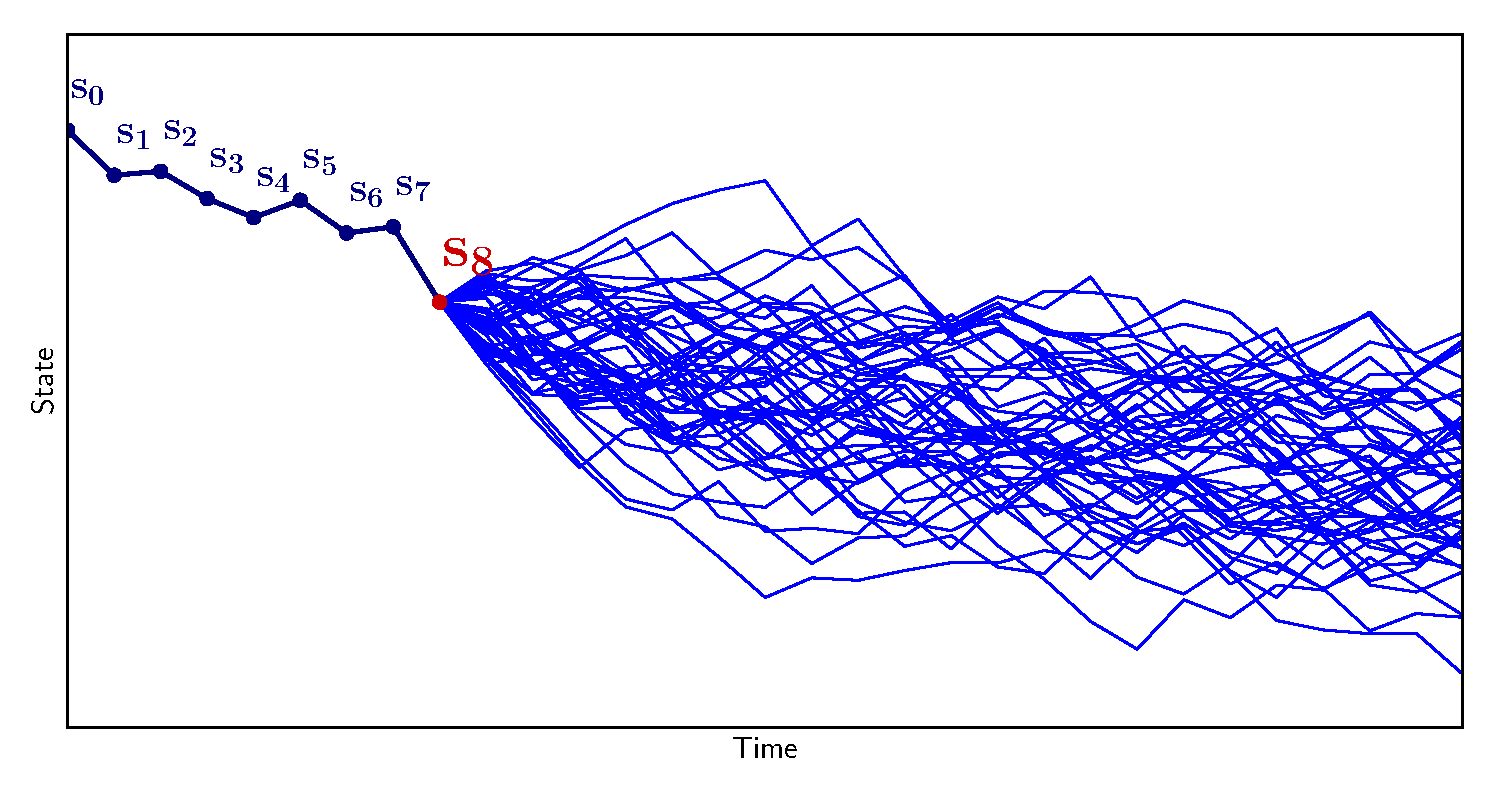
\includegraphics[width=\FS\textwidth,clip]{Codes/Basics/Markov8.eps}
        }%
              \only<14>
        {%
          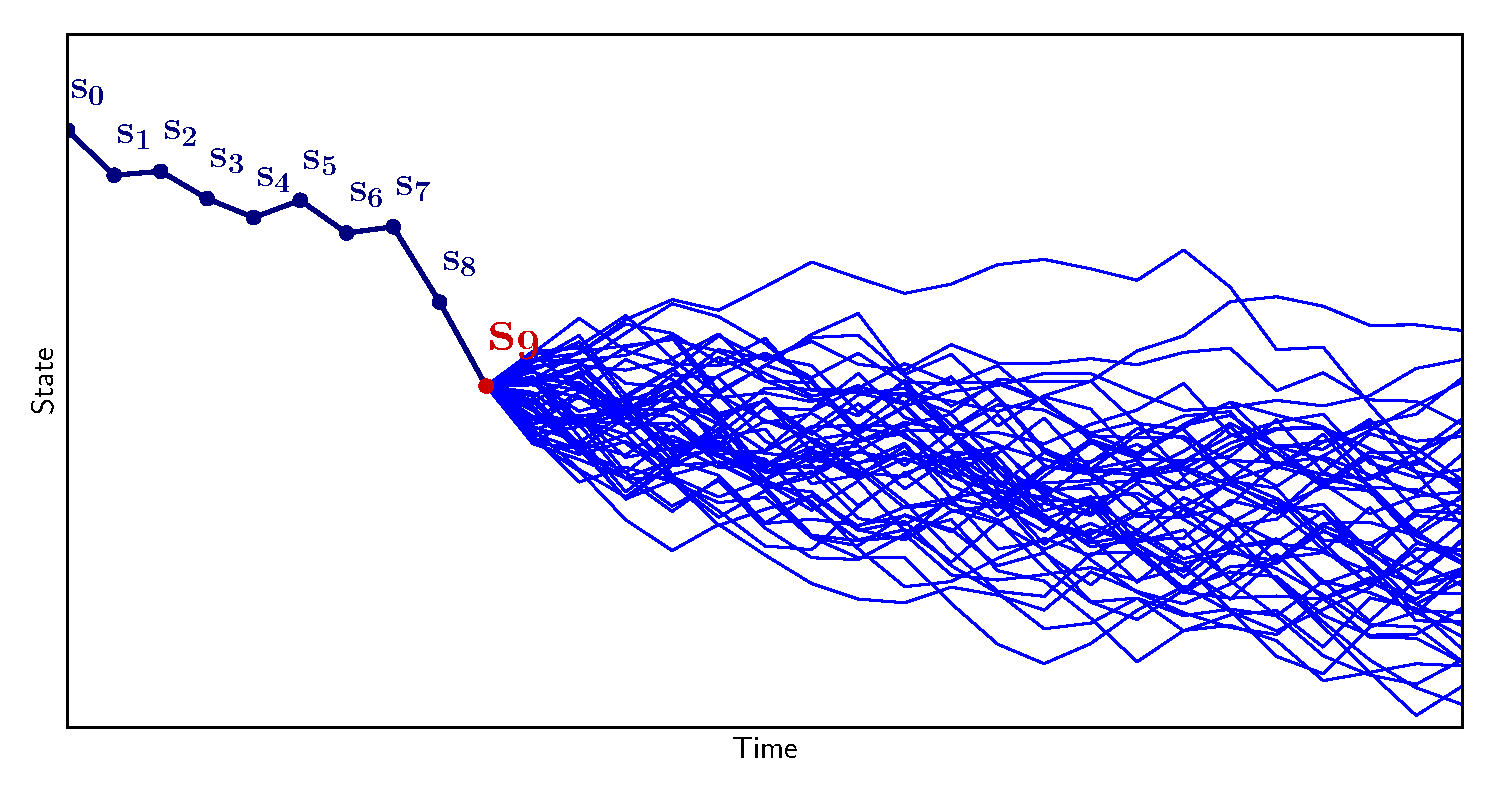
\includegraphics[width=\FS\textwidth,clip]{Codes/Basics/Markov9.eps}
        }%
              \only<15->
        {%
          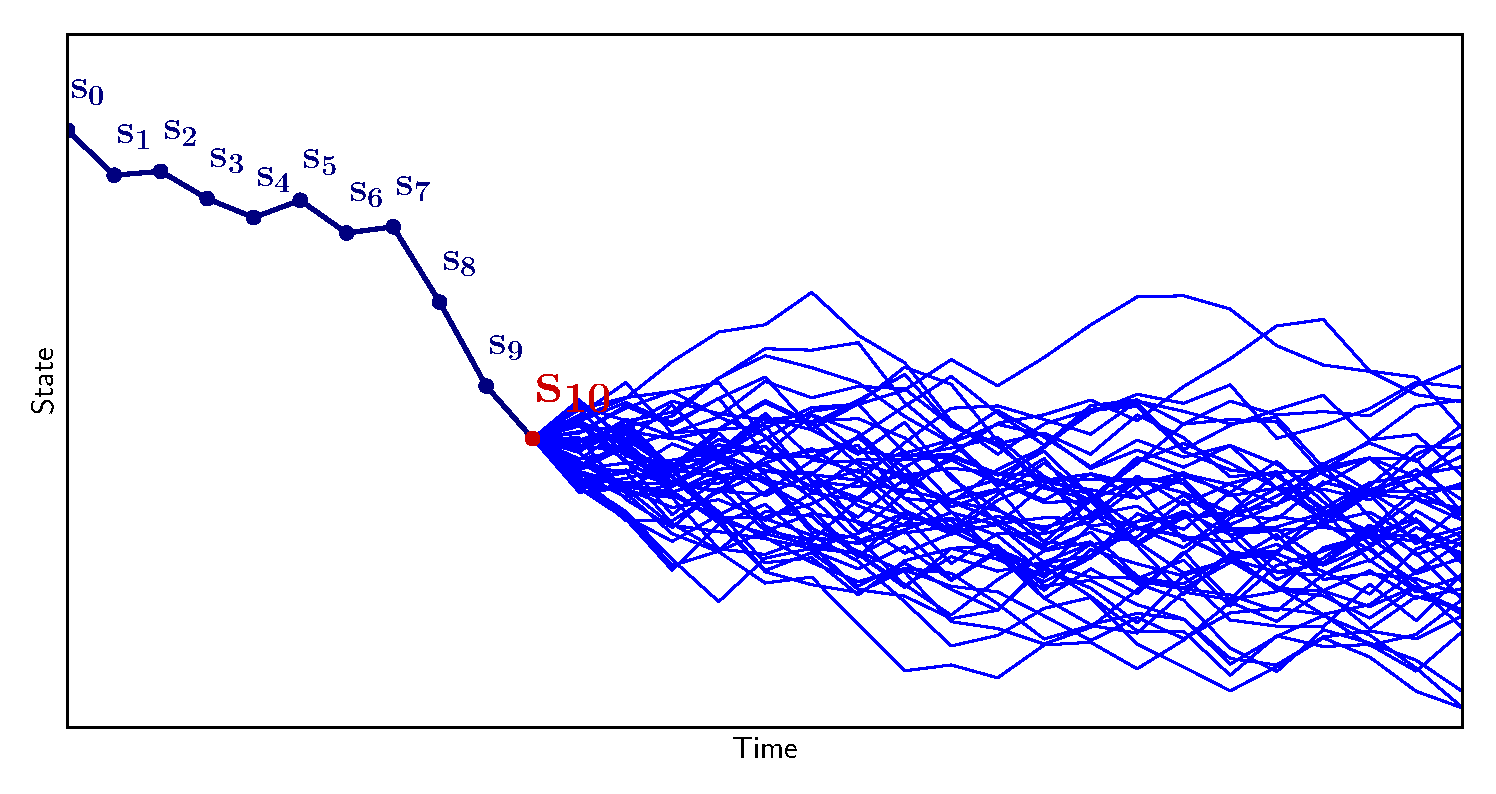
\includegraphics[width=\FS\textwidth,clip]{Codes/Basics/Markov10.eps}
        }%        
        \end{figure}
        \end{overlayarea}
        
%\begin{overlayarea}{\textwidth}{0.55\textheight}
%\only<5->{
%\begin{figure}
%\newcommand{\FS}{0.7}
%\includegraphics<1-5>[width=\FS\textwidth,clip]{Codes/Basics/Markov0.eps}
%\includegraphics<6>[width=\FS\textwidth,clip]{Codes/Basics/Markov1.eps}
%\includegraphics<7>[width=\FS\textwidth,clip]{Codes/Basics/Markov2.eps}
%\includegraphics<8>[width=\FS\textwidth,clip]{Codes/Basics/Markov3.eps}
%\includegraphics<9>[width=\FS\textwidth,clip]{Codes/Basics/Markov4.eps}
%\includegraphics<10>[width=\FS\textwidth,clip]{Codes/Basics/Markov5.eps}
%\includegraphics<11>[width=\FS\textwidth,clip]{Codes/Basics/Markov6.eps}
%\includegraphics<12>[width=\FS\textwidth,clip]{Codes/Basics/Markov7.eps}
%\includegraphics<13>[width=\FS\textwidth,clip]{Codes/Basics/Markov8.eps}
%\includegraphics<14>[width=\FS\textwidth,clip]{Codes/Basics/Markov9.eps}
%\includegraphics<15->[width=\FS\textwidth,clip]{Codes/Basics/Markov10.eps}
%\end{figure}
%}
%\end{overlayarea}



\end{frame}


\begin{frame}{\normalsize More on Markov States}
\footnotesize

\begin{overlayarea}{\textwidth}{0.8\textheight}
\only<1-2>{
\textbf{Direct Observations}
\begin{itemize}
\item In many applications, defining a Markov state is difficult: unknown, too complex, $\infty$-dimensional, etc
\item A long-enough history of past observations (and actions) is often (assumed to be) a Markov state
\item E.g. sequence of $n$ video frames + sensors measurements + actions is treated as Markov state in vision-based robotics
\end{itemize}
\vspace{.5cm}
\visible<2->{
\textbf{Belief State}
\begin{itemize}
\item We know our state \textit{structure} (what it is), but cannot observe it directly
\item Construct ``Data $\rightarrow$ Markov State", but we have imperfect knowledge
\item Belief state is the probability (density, measure) of $\vect s_k$
\item We can build optimal decision policies based on belief states and incorporate our imperfect knowledge in our decisions
\end{itemize}
}}
\only<3->{
\textbf{Latent State} (aka embeddings or compressed representations)
\begin{itemize}
\item Digest data into a Markov state (ML learns / proposes a state ``on its own")
\item TMBK, it is easier if assuming deterministic time evolution
\item Latent State$\rightarrow$Decision is a form of ``compression" (dimensionality reduction)
\item Building latent states efficient for decision making is ongoing research
\end{itemize}
\vspace{.5cm}
\visible<4->{
\textbf{State Observers}
\begin{itemize}
\item Standard term in classical system theory
\item Model-based construction of data$\rightarrow$(Markov) state 
\item Kalman filters ``family", Bayesian estimation, etc.
\end{itemize}
}}
\end{overlayarea}
\end{frame}

\begin{frame}{\normalsize Markov Decision Process (MDP)}
\footnotesize
\vspace{-.5cm}
\begin{overlayarea}{\textwidth}{0.5\textheight}
\only<1-12>{
\begin{itemize}
\item \textbf{State transition}: probability (density, measure) of landing on new state $\vect s_{+}$ from state $\vect s$ and with action $\vect a$:
\begin{align*}
\mathrm{P}\left[\,\vect s_{+}\, |\, \vect s,\vect a\,\right]
\end{align*}
\vspace{-.75cm}
\item \visible<2->{\textbf{Instantenuous performance}: 
\begin{align*}
L\left(\vect s,\vect a\right) = \text{Utility} - \cmatr{ccc}{0&\text{if}&\text{Constraints respected} \\
\infty&\text{if}&\text{Constraints violated} }
\end{align*}}
\vspace{-.5cm}
\item \visible<3->{\textbf{Policy}: function $\vect\pi\,:\, \text{state} \rightarrow \text{action}$}
\end{itemize}
}
\only<13->{

\begin{columns}[t]
\column{0.6\textwidth}
\begin{figure}
\newcommand{\FS}{1}
\includegraphics<13>[width=\FS\textwidth,clip]{Codes/Basics/MDPPerf0.eps}
\includegraphics<14>[width=\FS\textwidth,clip]{Codes/Basics/MDPPerf1.eps}
\includegraphics<15>[width=\FS\textwidth,clip]{Codes/Basics/MDPPerf2.eps}
\includegraphics<16>[width=\FS\textwidth,clip]{Codes/Basics/MDPPerf3.eps}
\includegraphics<17>[width=\FS\textwidth,clip]{Codes/Basics/MDPPerf4.eps}
\includegraphics<18>[width=\FS\textwidth,clip]{Codes/Basics/MDPPerf5.eps}
\includegraphics<19>[width=\FS\textwidth,clip]{Codes/Basics/MDPPerf6.eps}
\includegraphics<20>[width=\FS\textwidth,clip]{Codes/Basics/MDPPerf7.eps}
\includegraphics<21>[width=\FS\textwidth,clip]{Codes/Basics/MDPPerf8.eps}
\includegraphics<22->[width=\FS\textwidth,clip]{Codes/Basics/MDPPerf9.eps}
\end{figure}
\column{0.3\textwidth}
\vspace{-.5cm}
\center$J\left(\vect \pi\right)$\\
\vspace{-.3cm}
\begin{figure}
\newcommand{\FS}{1}
\includegraphics<13>[width=\FS\textwidth,clip]{Codes/Basics/PolicyPerf0.eps}
\includegraphics<14>[width=\FS\textwidth,clip]{Codes/Basics/PolicyPerf1.eps}
\includegraphics<15>[width=\FS\textwidth,clip]{Codes/Basics/PolicyPerf2.eps}
\includegraphics<16>[width=\FS\textwidth,clip]{Codes/Basics/PolicyPerf3.eps}
\includegraphics<17>[width=\FS\textwidth,clip]{Codes/Basics/PolicyPerf4.eps}
\includegraphics<18>[width=\FS\textwidth,clip]{Codes/Basics/PolicyPerf5.eps}
\includegraphics<19>[width=\FS\textwidth,clip]{Codes/Basics/PolicyPerf6.eps}
\includegraphics<20>[width=\FS\textwidth,clip]{Codes/Basics/PolicyPerf7.eps}
\includegraphics<21>[width=\FS\textwidth,clip]{Codes/Basics/PolicyPerf8.eps}
\includegraphics<22->[width=\FS\textwidth,clip]{Codes/Basics/PolicyPerf9.eps}
\end{figure}
\end{columns}
}
\end{overlayarea}
\vspace{-1cm}

\begin{overlayarea}{\textwidth}{0.45\textheight}
\only<4-11>{


  \begin{overlayarea}{\textwidth}{1\textheight}
    \begin{figure}
    \newcommand{\FS}{0.7}
      \centering
      \only<4>
        {%
          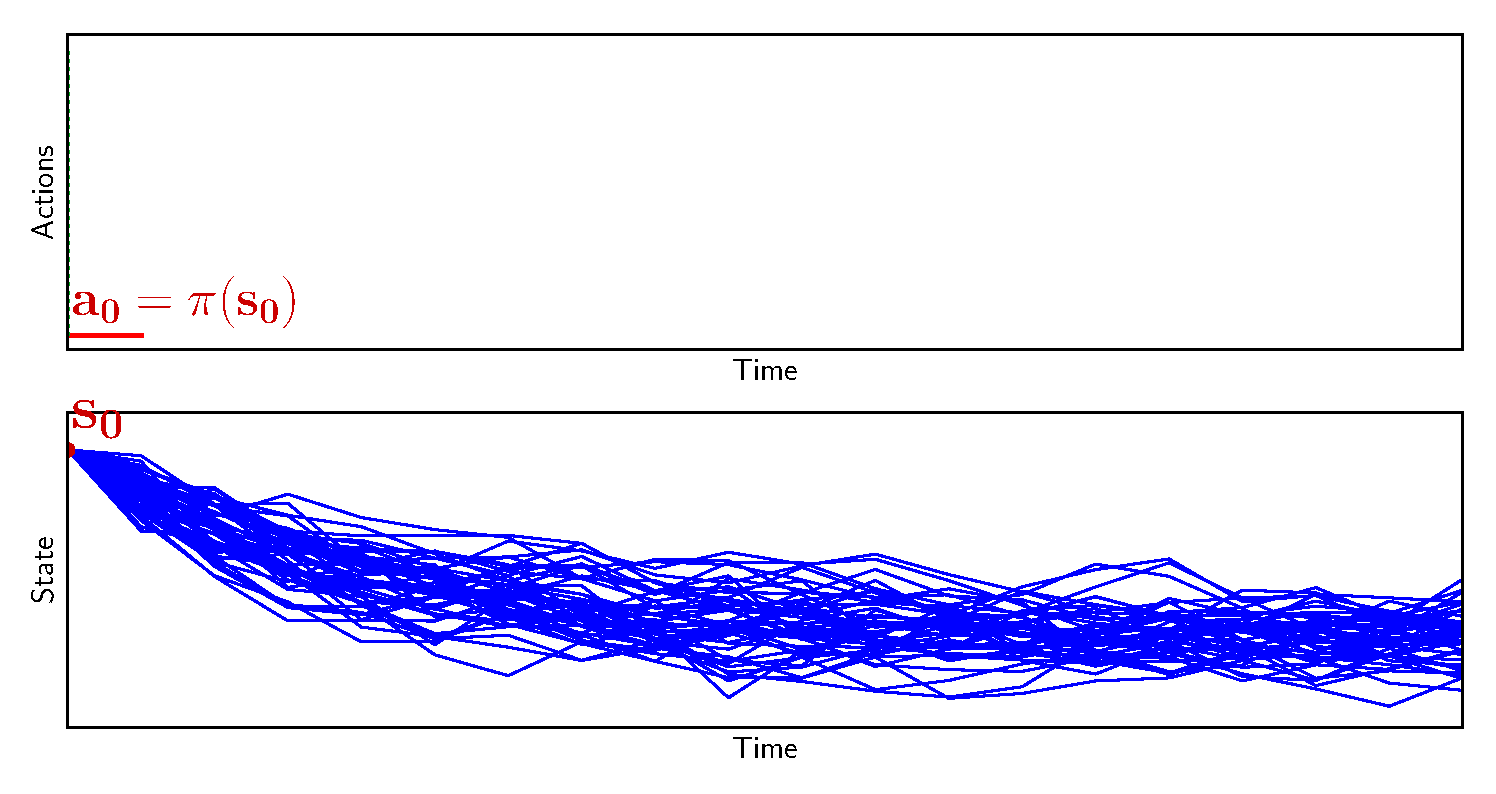
\includegraphics[width=\FS\textwidth,clip]{Codes/Basics/MDP0.eps}
        }%
              \only<5>
        {%
          \includegraphics[width=\FS\textwidth,clip]{Codes/Basics/MDP1.eps}
        }%
              \only<6>
        {%
          \includegraphics[width=\FS\textwidth,clip]{Codes/Basics/MDP2.eps}
        }%
              \only<7>
        {%
          \includegraphics[width=\FS\textwidth,clip]{Codes/Basics/MDP3.eps}
        }%
              \only<8>
        {%
          \includegraphics[width=\FS\textwidth,clip]{Codes/Basics/MDP4.eps}
        }%
              \only<9>
        {%
          \includegraphics[width=\FS\textwidth,clip]{Codes/Basics/MDP5.eps}
        }%
              \only<10>
        {%
          \includegraphics[width=\FS\textwidth,clip]{Codes/Basics/MDP6.eps}
        }%
              \only<11>
        {%
          \includegraphics[width=\FS\textwidth,clip]{Codes/Basics/MDP7.eps}
        }%
        \end{figure}
        \end{overlayarea}
}
%\begin{figure}
%\newcommand{\FS}{0.7}
%\includegraphics<4>[width=\FS\textwidth,clip]{Codes/Basics/MDP0.eps}
%\includegraphics<5>[width=\FS\textwidth,clip]{Codes/Basics/MDP1.eps}
%\includegraphics<6>[width=\FS\textwidth,clip]{Codes/Basics/MDP2.eps}
%\includegraphics<7>[width=\FS\textwidth,clip]{Codes/Basics/MDP3.eps}
%\includegraphics<8>[width=\FS\textwidth,clip]{Codes/Basics/MDP4.eps}
%\includegraphics<9>[width=\FS\textwidth,clip]{Codes/Basics/MDP5.eps}
%\includegraphics<10>[width=\FS\textwidth,clip]{Codes/Basics/MDP6.eps}
%\includegraphics<11->[width=\FS\textwidth,clip]{Codes/Basics/MDP7.eps}
%\end{figure}
%}

\only<12->{
\vspace{0.75cm}
\begin{itemize}
\item \textbf{Policy performance}: expected long-term sum of (discounted) utility
\begin{align*}
J\left(\vect\pi\right)=\mathrm{E}\left[\left.\sum_{k=0}^\infty\,\gamma^kL\left(\vect s_k,\vect a_k\right)\,\right |\,\vect a_k=\vect\pi\left(\vect s_k\right)  \right]
\end{align*}
\begin{flushright} for $0<\gamma\leq 1$. \end{flushright}
\item  \visible<23->{\textbf{Optimal policy}: is maxing out $J\left(\vect\pi\right)$, i.e.
\begin{align*}
\vect\pi^\star = \argmax_{\vect\pi}\, J\left(\vect\pi\right)
\end{align*} }
\end{itemize}
}
\end{overlayarea}


\end{frame}


%\begin{frame}{\normalsize Markov State and MDPs}
%\footnotesize
%\begin{center}
%\textit{The Markov state should include all relevant information for taking decisions} 
%\end{center}
%
%TODO: forecasts are part of the Markov state, POMDP, Rock-paper-scissor example...
%\end{frame}

\begin{frame}{\normalsize Solving MDPs}
\footnotesize
BUILD THIS 
%
%\begin{columns}
%\column{0.5\textwidth}
%\begin{figure}
%\newcommand{\FS}{1}
%%\includegraphics<13>[width=\FS\textwidth,clip]{Codes/Basics/MDPPerf0.eps}
%%\includegraphics<14>[width=\FS\textwidth,clip]{Codes/Basics/MDPPerf1.eps}
%%\includegraphics<15>[width=\FS\textwidth,clip]{Codes/Basics/MDPPerf2.eps}
%\includegraphics[width=\FS\textwidth,clip]{Codes/Basics/MDPPerf3.eps}
%%\includegraphics<17>[width=\FS\textwidth,clip]{Codes/Basics/MDPPerf4.eps}
%%\includegraphics<18>[width=\FS\textwidth,clip]{Codes/Basics/MDPPerf5.eps}
%%\includegraphics<19>[width=\FS\textwidth,clip]{Codes/Basics/MDPPerf6.eps}
%%\includegraphics<20>[width=\FS\textwidth,clip]{Codes/Basics/MDPPerf7.eps}
%%\includegraphics<21>[width=\FS\textwidth,clip]{Codes/Basics/MDPPerf8.eps}
%%\includegraphics<22->[width=\FS\textwidth,clip]{Codes/Basics/MDPPerf9.eps}
%\end{figure}
%\column{0.5\textwidth}
%$J\left(\vect\pi\right)$ is assuming an underlying initial state distribution
%\end{columns}
%
%
\end{frame}
%
%
%\begin{frame}{\normalsize The Role of the Value Functions}
%\footnotesize
%
%
%\end{frame}
%
%
%\begin{frame}{\normalsize Computing an Optimal Polivy}
%\footnotesize
%
%
%\end{frame}


\section{Solving MDPs}

\begin{frame}{\normalsize Dynamic Programming}
\footnotesize

\end{frame}

\begin{frame}{\normalsize Repeated Planning}
\footnotesize

\end{frame}

\begin{frame}{\normalsize Reinforcement Learning}
\footnotesize

\end{frame}

\section{Using Data in Decision Making}

\begin{frame}{\normalsize Model-Free Reinforcement Learning}
\footnotesize
\begin{center}
\textit{Learn a policy purely via interactions with the real world}
\end{center}
\begin{itemize}
\item  \textbf{Policy} is parametrized, i.e. $\vect a= \vect\pi_{\vect \theta}\left(\vect s\right)$ for parameter $\vect \theta$, e.g. via a DNN
\item  \textbf{Performance} $J\left(\vect\pi_{\vect\theta}\right)$ \textit{can be} evaluated from data\\
%\begin{figure}
\vspace{-.4cm}
\hspace{7cm}\includegraphics[width=.15\textwidth,clip]{Codes/Basics/PolicyPerf9.eps}
%\end{figure}
\item \visible<3->{\textbf{Gradient} $\nabla_{\vect \theta}J\left(\vect\pi_{\vect \theta}\right)$ is evaluated from data using actor-critic techniques
\begin{itemize}
\footnotesize
\item actor is the policy $\vect\pi_{\vect \theta}$
\item critic assesses ``which action we should ``get more of" in each state %$\vect s$"\\$\rightarrow$ Expected value provides a direction in policy parameters $\vect \theta$
\item requires ``exploration" (aka ``excitation" in dynamic systems terminology)
\end{itemize}}
\item \visible<4->{\textbf{Update} of policy parameters e.g. using:
\begin{align*}
\vect \theta\leftarrow \vect \theta + \alpha \nabla_{\vect \theta}J\left(\vect\pi_{\vect \theta}\right)
\end{align*} 
for some $\alpha > 0$ + a lot of heuristics}
\end{itemize}

\end{frame}

\begin{frame}{\normalsize Model-Free Reinforcement Learning}
\footnotesize

\newcommand{\Sys}{\vspace{-0.25cm}\includegraphics[width=1\textwidth,clip]{Figures/SmartHouse.eps}}

\tikzstyle{Sys_block} = [rectangle, draw, fill=none,  text width=3.cm, text centered, rounded corners, minimum height=4em,inner sep=2pt]
\tikzstyle{Opt_block} = [rectangle, draw, fill=myLightGreen,  text width=2.5cm,  text centered, rounded corners]
\tikzstyle{RL_block} = [rectangle, draw, fill=myOrange,  text width=2.5cm,  text centered, rounded corners]
\tikzstyle{Util_block} = [rectangle, draw, fill=myLightBlue,  text width=3.5cm,  text centered, rounded corners]
\tikzstyle{Const_block} = [rectangle, draw, fill=myLightRed,  text width=3.5cm,  text centered, rounded corners]
\tikzstyle{line} = [draw, -latex']


\begin{tikzpicture}[->,>=stealth']

\node [Sys_block] (sys0) {\Sys};


 \node [Opt_block, left of=sys0, node distance = 4cm] (opt0) {
 \begin{minipage}[c]{2.5cm}
 \center
\textbf{Policy} $\vect\pi_{\vect\theta}$
\end{minipage}
 };
 
  \node [RL_block, left of=opt0, node distance = 4cm] (RL0) {
 \begin{minipage}[c]{2.5cm}
 \center
RL estimates\\$\nabla_{\vect\theta}J\left(\vect\pi_{\vect\theta}\right)$
\end{minipage}
 };

  \node [Util_block, below of=RL0, node distance = 1.6cm] (util0) {
 \begin{minipage}[c]{3.5cm}
 \center
Utility
\end{minipage}
 };


  \node [Const_block, above of=RL0, node distance = 1.6cm] (limit0) {
 \begin{minipage}[c]{3.5cm}
 \center
Constraints
\end{minipage}
 };

 
 \path  (sys0) edge[bend left=20]  node[anchor=north] {Info} (opt0)
 (opt0) edge[bend left=20]  node[anchor=south] {Action} (sys0);
 \path (util0) edge[<->]  node[anchor=east] {} (RL0);
 \path (limit0) edge[<->] node[anchor=east] {} (RL0);
  \path  %(sys0) edge[bend left=30]  node[anchor=north] {Info} (RL0)
 (sys0) edge[bend right=30]  node[anchor=north] {Data} (RL0);  
  \path (RL0) edge node[anchor=north] {New $\vect\theta$} (opt0);
\end{tikzpicture}

\vspace{.5cm}
\visible<2->{
\textbf{Remarks}
\begin{itemize}
\item Can be run without building any model of the real world
\item RL cumulates data (actions \& info) and treats them ``at large scale" %to estimate $\nabla_{\vect\theta}J\left(\vect\pi_{\vect\theta}\right)$
\item RL is usually more efficient than exploring $J\left(\vect\pi_{\vect \theta}\right)$ via ``perturbations" of $\vect\theta$\\\tiny{(numerical gradient, GA, BO, etc)}
\end{itemize}
}

\end{frame}


\begin{frame}{\normalsize Policy from Data-Driven Models}
\footnotesize
\vspace{-.5cm}
\begin{itemize}
\item \textbf{Build (AI) model}, e.g. as
\begin{itemize}
\footnotesize
\item Probabilistic: $\hat{\mathrm{P}}_{\vect\theta}\left[\,\vect s_+\,|\,\vect s,\vect a\,\right]$ $\rightarrow$ e.g. via Max Likelihood of $\hat{\mathrm{P}}_{\vect\theta}$ over data
\item Point prediction: $\hat{\vect s}_+ = \vect f_{\vect\theta}\left(\vect s,\vect a\right)$ $\rightarrow$ e.g. via fitting on data (LS, Lasso, etc)
\end{itemize}
\item \visible<2->{\textbf{Build policy} from $\vect\pi_{\vect \theta}=\argmax_{\vect \pi}\,\hat J_{\vect\theta}\left(\vect \pi\right)$, i.e optimal for the model}
\item \visible<3->{\textbf{Transfer} policy into the real world, hope for the best...}
\end{itemize}


\newcommand{\Sys}{\vspace{-0.25cm}\includegraphics[width=1\textwidth,clip]{Figures/SmartHouse.eps}}

\tikzstyle{Sys_block} = [rectangle, draw, fill=none,  text width=3.cm, text centered, rounded corners, minimum height=4em,inner sep=2pt]
\tikzstyle{Obj_block} = [rectangle, draw, fill=myLightRed,  text width=3.25cm, text centered, rounded corners, minimum height=4em,inner sep=2pt]
\tikzstyle{Opt_block} = [rectangle, draw, fill=myLightGreen,  text width=3cm,  text centered, rounded corners]
\tikzstyle{ID_block} = [rectangle, draw, fill=myLightBlue,  text width=3cm, text centered, rounded corners]    
\tikzstyle{line} = [draw, -latex']

\begin{tikzpicture}[->,>=stealth']

\node [Sys_block] (sys0) {\Sys};

\node [ID_block, left of=sys0, node distance = 4.75cm] (ID0) {
 \begin{minipage}[c]{3cm}
\textbf{ML model} e.g.
\begin{align*}
\hat{\vect{s}}_{+} \sim \hat{\mathrm P}_{\vect{\theta}}\left[\cdot\,|\,\vect{s},\vect{a}\right]
\end{align*}
\vspace{-.75cm}
\flushright fitting real-world data
\end{minipage}
 };


 \visible<2->{
 \node [Opt_block, below of=ID0, node distance = 2.5cm] (opt0) {
 \begin{minipage}[c]{3cm}
 \center
\textbf{Build Policy}
 \vspace{-0.2cm}
\begin{align*}
\vect\pi_{\vect \theta}
\end{align*}
 \vspace{-0.5cm}\\
optimal for ML model
\end{minipage}
 };
 
 \node [Obj_block, left of=opt0, node distance = 4cm] (Obj0) {
 \begin{minipage}[c]{3.25cm}
 \center
\textbf{Utility \& Constraints}
\vspace{-.5cm}\\
\begin{align*}
L\left(\vect s,\vect a\right)
\end{align*}
%(possibly unbounded)
\end{minipage}
 };}
 
 \path 
 (sys0) edge  node[anchor=center,xshift=-.5em] {
  \begin{minipage}[c]{1cm}
  \center
 Data\\ knowledge
 \end{minipage}} (ID0);
 \visible<2->{  \path (ID0) edge[bend left=20]  node[anchor=west] {Virtual data} (opt0);}
  \visible<2->{ \path (opt0) edge[bend left=20]  node[anchor=east] {Actions} (ID0);}
 \visible<3->{  \path (opt0) edge[bend right=20]  node[anchor=west,xshift=1em] {Transfer} (sys0);}
 \visible<2->{   \path (Obj0) edge  node[anchor=south] {} (opt0);}
  
\end{tikzpicture}

\center
 \visible<4->{$\vect\pi_{\vect\theta}$ can be built using RL, ADP, Direct gradient evaluation, etc.}\\
 \visible<5->{\textcolor{myBlue2}{\textbf{Labelled Sim2Real in some communities} } }
\end{frame}

\begin{frame}{\normalsize Repeated Planning from Data-Driven Models}
\footnotesize


\begin{itemize}
\item \textbf{Build (AI) model}
\item \visible<2->{\textbf{Build action plan} at every time $k$ optimized over horizon $N$ for AI model}
\item \visible<3->{\textbf{Apply} first action $\vect a_k$ into the real world, hope for the best...}
\end{itemize}

\newcommand{\Sys}{\vspace{-0.25cm}\includegraphics[width=1\textwidth,clip]{Figures/SmartHouse.eps}}

\tikzstyle{Sys_block} = [rectangle, draw, fill=none,  text width=3.cm, text centered, rounded corners, minimum height=4em,inner sep=2pt]
\tikzstyle{Obj_block} = [rectangle, draw, fill=myLightRed,  text width=3.25cm, text centered, rounded corners, minimum height=4em,inner sep=2pt]
\tikzstyle{Opt_block} = [rectangle, draw, fill=myLightGreen,  text width=3cm,  text centered, rounded corners]
\tikzstyle{ID_block} = [rectangle, draw, fill=myLightBlue,  text width=3cm, text centered, rounded corners]    
\tikzstyle{line} = [draw, -latex']

\begin{tikzpicture}[->,>=stealth']

\node [Sys_block] (sys0) {\Sys};

\node [ID_block, left of=sys0, node distance = 4.75cm] (ID0) {
 \begin{minipage}[c]{3cm}
\textbf{ML model} e.g.
\begin{align*}
\hat{\vect{s}}_{+} \sim \hat{\mathrm P}_{\vect{\theta}}\left[\cdot\,|\,\vect{s},\vect{a}\right]
\end{align*}
\vspace{-.75cm}
\flushright fitting real-world data
\end{minipage}
 };


 \visible<2->{
 \node [Opt_block, below of=ID0, node distance = 2.5cm] (opt0) {
 \begin{minipage}[c]{3cm}
 \center
\textbf{Build Action Plan}\\
 \vspace{-0.6cm}
\begin{align*}
\vect a_{k,\ldots,k+N}
\end{align*}
 \vspace{-0.5cm}\\
optimized for model
\end{minipage}
 };
 
 \node [Obj_block, left of=opt0, node distance = 4cm] (Obj0) {
 \begin{minipage}[c]{3.25cm}
 \center
\textbf{Utility \& Constraints}
\vspace{-.5cm}\\
\begin{align*}
L\left(\vect s,\vect a\right)
\end{align*}
%(possibly unbounded)
\end{minipage}
 };}
 
 \path 
 (sys0) edge  node[anchor=center,xshift=-.5em] {
  \begin{minipage}[c]{1cm}
  \center
 Data\\ knowledge
 \end{minipage}} (ID0);
 \visible<2->{  \path (sys0) edge[bend right=40]  node[anchor=south] {Current state (time $k$)} (ID0);}
 \visible<2->{  \path (ID0) edge[bend left=20]  node[anchor=west] {Predictions} (opt0);}
  \visible<2->{ \path (opt0) edge[bend left=20]  node[anchor=east] {Action Plan} (ID0);}
 \visible<3->{  \path (opt0) edge[bend right=20]  node[anchor=west,xshift=1em] {Apply $\vect a_k$} (sys0);}
 \visible<2->{   \path (Obj0) edge  node[anchor=south] {} (opt0);}
  
\end{tikzpicture}

\center
 \visible<4->{$\vect a_{k,\ldots,k+N}$ built using Nonlinear Prog., Multi-stage Stochastic Prog., etc}\\
 \visible<5->{\textcolor{myBlue2}{\textbf{Many labels} } }


\end{frame}

\begin{frame}{\normalsize Model Fitting \& Decision Optimality}
\footnotesize

\newcommand{\Sys}{\vspace{-0.25cm}\includegraphics[width=1\textwidth,clip]{Figures/SmartHouse.eps}}

\tikzstyle{Sys_block} = [rectangle, draw, fill=none,  text width=3.cm, text centered, rounded corners, minimum height=4em,inner sep=2pt]
\tikzstyle{Obj_block} = [rectangle, draw, fill=myLightRed,  text width=3.25cm, text centered, rounded corners, minimum height=4em,inner sep=2pt]
\tikzstyle{Opt_block} = [rectangle, draw, fill=myLightGreen,  text width=3cm,  text centered, rounded corners]
\tikzstyle{ID_block} = [rectangle, draw, fill=myLightBlue,  text width=3cm, text centered, rounded corners]    
\tikzstyle{line} = [draw, -latex']

\begin{tikzpicture}[->,>=stealth']

\node [Sys_block] (sys0) {\Sys};

\node [ID_block, left of=sys0, node distance = 4.75cm] (ID0) {
 \begin{minipage}[c]{3cm}
\textbf{ML model} e.g.
\begin{align*}
\hat{\vect{s}}_{+} \sim \hat{\mathrm P}_{\vect{\theta}}\left[\cdot\,|\,\vect{s},\vect{a}\right]
\end{align*}
\vspace{-.75cm}
\flushright fitting real-world data
\end{minipage}
 };



 \node [Opt_block, below of=ID0, node distance = 2.5cm] (opt0) {
 \begin{minipage}[c]{3cm}
 \center
\textbf{Build Decisions}
\begin{itemize}
\scriptsize
\item Policy
\item Rep. planning
\end{itemize}
\end{minipage}
 };
 
 \node [Obj_block, left of=opt0, node distance = 4cm] (Obj0) {
 \begin{minipage}[c]{3.25cm}
 \center
\textbf{Utility \& Constraints}
%\vspace{-.5cm}\\
%\begin{align*}
%L\left(\vect s,\vect a\right)
%\end{align*}
%(possibly unbounded)
\end{minipage}
 };
 
 \path 
 (sys0) edge  node[anchor=center,xshift=-.5em] {
  \begin{minipage}[c]{1cm}
  \center
 Data\\ knowledge
 \end{minipage}} (ID0);
% \path (sys0) edge[bend right=40]  node[anchor=south] {Decisions} (ID0);
 \path (ID0) edge[bend left=20]  node[anchor=west] {Predictions} (opt0);
\path (opt0) edge[bend left=20]  node[anchor=east] {Actions} (ID0);
\path (opt0) edge[bend right=20]  node[anchor=west,xshift=1em] {Policy or actions} (sys0);
 \path (Obj0) edge  node[anchor=south] {} (opt0);
  
\end{tikzpicture}




\begin{columns}[c]
\column{0.5\textwidth}
\visible<2->{E.g. for $\vect s,\vect a$ given}\\
\vspace{-.25cm}
\begin{figure}
\includegraphics<2->[width=\textwidth,clip]{Codes/Basics/Model.eps}
\end{figure}
\column{0.5\textwidth}
\visible<3->{
\begin{block}{}
\center
$\vect\theta$ that best fits model to real data \\
$\Downarrow$\\
Best $\vect\theta$ for taking decisions in the real world?
\end{block}}
\begin{overlayarea}{\textwidth}{0.25\textheight}
\only<4>{
\begin{alertblock}{}
\textbf{In general no:} equations describing best $\vect\theta$ for fitting the model to data $\neq$ equations describing $\vect\theta$ that yields the best decisions
\end{alertblock}
}
\only<5->{\begin{center} In other words, the best model tuning for fitting the data is not (necessarily$^1$) the best model tuning for taking decisions. Unless the model is exact!\end{center}
\visible<6->{\tiny $^1$ it is for a very special class of decision problems}
}
\end{overlayarea}

\end{columns}
\end{frame}


\begin{frame}{\normalsize RL over Decision Making}
\footnotesize
\newcommand{\Sys}{\vspace{-0.25cm}\includegraphics[width=1\textwidth,clip]{Figures/SmartHouse.eps}}

%\vspace{-1cm}
\tikzstyle{Sys_block} = [rectangle, draw, fill=none,  text width=3.cm, text centered, rounded corners, minimum height=4em,inner sep=2pt]
\tikzstyle{Obj_block} = [rectangle, draw, fill=myLightRed,  text width=3.2cm, text centered, rounded corners, minimum height=4em,inner sep=2pt]
\tikzstyle{Opt_block} = [rectangle, draw, fill=myLightGreen,  text width=3cm,  text centered, rounded corners]
\tikzstyle{ID_block} = [rectangle, draw, fill=myLightBlue,  text width=3cm, text centered, rounded corners]    

\tikzstyle{RL_block} = [rectangle, draw, fill=none,  text width=3.cm, text centered, rounded corners, minimum height=4em,inner sep=2pt]

\tikzstyle{line} = [draw, -latex']

\begin{tikzpicture}[->,>=stealth']

\node [Sys_block] (sys0) {\Sys};

\node [ID_block, left of=sys0, node distance = 5cm] (ID0) {
 \begin{minipage}[c]{3cm}
% \vspace{-0.2cm}
\textbf{ML model} e.g.
\begin{align*}
\hat{\vect{s}}_{+} \sim \hat{\mathrm P}_{\vect{\theta}}\left[\cdot\,|\,\vect{s},\vect{a}\right]
\end{align*}
\end{minipage}
 };

\visible<3->{
\node [RL_block, above of=ID0, node distance = 2.0cm] (RL0) {
 \begin{minipage}[c]{3cm}
\textbf{RL} 
\vspace{-.25cm} 
\begin{align*}
\Delta\vect\theta = \alpha\nabla_{\vect\theta} J\left(\vect\pi_{\vect \theta}\right)
\end{align*}
\vspace{-.85cm}
\flushright from real data
\end{minipage}
 };}

 
 \node [Opt_block, below of=ID0, node distance = 2.5cm] (opt0) {
 \begin{minipage}[c]{3cm}
 \center
 \center
\textbf{Build Decisions}
\begin{itemize}
\scriptsize
\item Policy
\item Rep. planning
\end{itemize}
\end{minipage}
 };
 
 \node [Obj_block, left of=opt0, node distance = 4cm] (Obj0) {
 \begin{minipage}[c]{3.2cm}
 \center
\textbf{Utility \& Constraints}
\vspace{-.5cm}
\begin{overlayarea}{\textwidth}{0.1\textheight}
\only<1-3>{
\vspace{-.5cm}
\begin{align*}
L\left(\vect s,\vect a\right)
\end{align*}
}
\only<4->{
\vspace{-.5cm}
\begin{align*}
L_{\vect \theta}\left(\vect s,\vect a\right)
\end{align*}
}
\end{overlayarea}

\end{minipage}
 };

\visible<5->{
 \node [Obj_block, left of=RL0, node distance = 4cm] (Obj1) {
 \begin{minipage}[c]{3.2cm}
 \center
\textbf{Utility \& Constraints}
\vspace{-.25cm}
\begin{align*}
L\left(\vect s,\vect a\right)
\end{align*}
\end{minipage}
 };
}

 
 \path 
 (sys0) edge  node[anchor=center,xshift=-.5em] {
  \begin{minipage}[c]{1cm}
  \center
 Data\\ knowledge
 \end{minipage}} (ID0)
 (ID0) edge[bend left=20]  node[anchor=west] {Predictions} (opt0)
 (opt0) edge[bend left=20]  node[anchor=east] {Actions} (ID0)
 (opt0) edge[bend right=20]  node[anchor=west,xshift=1em] {Policy or actions} (sys0)
 (Obj0) edge  node[anchor=south] {} (opt0)
 ;
 
 \visible<3->{
 \path   (sys0) edge[bend right=20]  node[anchor=south west] {
  \begin{minipage}[c]{1cm}
  \center
 Data\\ knowledge
 \end{minipage}} (RL0)
  (RL0) edge  node[anchor=west] {$\Delta\vect\theta$} (ID0);}

 \visible<4->{\path    (RL0) edge[bend right=20]  node[anchor=south east] {$\Delta\vect\theta$} (Obj0);}
 \visible<5->{\path    (Obj1) edge[]  node[anchor=south east] {} (RL0);}


\visible<2->{\draw[blue,thick] ($(ID0.north east)+(+0.15,0.15)$)  rectangle ($(Obj0.south west)+(-0.15,-0.3)$);}
\end{tikzpicture}
\vspace{-.25cm}
\begin{itemize}
\item The model is not $\hat{\mathrm P}_{\vect \theta}$, it is the entire ``decision box"
\item Utility \& Constraints to build decisions from the predictions are part of the model
\item RL can tune the whole \textcolor{blue}{decision box}, from real data + true Utility \& Constraints 
\end{itemize}




\end{frame}

\begin{frame}{\normalsize What does it say about AID?}
\footnotesize
\begin{center}
\textit{We have discussed on the key concepts of decision making}
\end{center}
\begin{overlayarea}{\textwidth}{0.75\textheight}
\only<2>{
\begin{block}{}
\textbf{Markov state and RA3 (Data to Information)} (more in another talk)
\begin{itemize}
\item The problem of ``building" a \textbf{Markov state} for a given problem is tricky
\item Recent history of observation can play that role, but it is often too large
\item ``Compression" observations into a relevant, lower-dimensional ``latent state" is critical
\item How to build a latent state useful for decision is a key RQ
\end{itemize}
\end{block}
}
\only<3>{
\begin{block}{}
\textbf{Models for decision and RA5 (Training models for decision)} (more in another talk)
\begin{itemize}
\item Best model fit $\neq$ best model for decision
\item Decision-oriented model training is possible
\item More research needed 
\end{itemize}
\end{block}
}
\only<4>{
\begin{block}{}
\textbf{Repeated planning and RA7 (AI and formal decision tools)} (more in another talk)
\begin{itemize}
\item In practice, decisions are often taken from repeated planning
\item Complex relationship model accuracy - policy performance in that context
\item Theory explaining that relationship exists + methods to train repeated planning towards optimal decisions
\item More research needed 
\end{itemize}
\end{block}
}
\end{overlayarea}


\end{frame}


\begin{frame}{\normalsize AI for Decision Making}
\footnotesize

\huge

\center
There is a lot more to say...\\
but we will keep that for the future

\end{frame}

\end{document}

